\documentclass[11pt]{article}
\usepackage{graphicx}
\DeclareGraphicsRule{.tif}{png}{.png}{`convert #1 `dirname #1`/`basename #1 .tif`.png}
\usepackage{wrapfig}
\textwidth = 6.5 in
\textheight = 9 in
\oddsidemargin = 0.0 in
\evensidemargin = 0.0 in
\topmargin = 0.0 in
\headheight = 0.0 in
\headsep = 0.0 in
\parskip = 0.2in
\parindent = 0.0in
\usepackage{setspace}
\singlespacing

\usepackage{titlesec}
\usepackage{paralist} %compactenum

%\newtheorem{theorem}{Theorem}
%\newtheorem{corollary}[theorem]{Corollary}
%\newtheorem{definition}{Definition}
\usepackage{tipa}
\usepackage{amsfonts}
\usepackage[mathscr]{eucal}

\titlespacing*{\section}{0cm}{1mm}{-3mm}
\titlespacing*{\subsection}{0cm}{-3mm}{-3mm}
% Use the natbib package for the bibliography
\usepackage[round]{natbib}
\bibliographystyle{apalike}
\newcommand{\exampleMacro}[1]{\mu_{#1}}


\renewcommand{\section}[2]{%
\bigskip
\begin{center}
\begin{Large}
\normalfont\scshape #2
\medskip
\end{Large}
\end{center}}

\renewcommand{\subsection}[1]{%
\noindent{\large\scshape \underline{#1}}:}

\renewcommand{\subsubsection}[1]{%
\noindent\textbf{#1}:}


\usepackage{xspace}
%\usepackage{ulem}
\usepackage{url}
\usepackage{hyperref}


\hypersetup{backref,  pdfpagemode=FullScreen,  linkcolor=blue, citecolor=red, colorlinks=true, hyperindex=true}

\newcommand{\boot}[1]{X^{(#1)}}
\newcommand{\sdLL}[1]{\hat{\sigma_{#1}}}
\newcommand{\sdLLBoot}[2]{\hat{\sigma_{#1}}^{(#2)}}
\newcommand{\like}{\ell}
\newcommand{\lnL}{\ln L}
\newcommand{\expectation}{{\mathbb{E}}}
\newcommand{\expect}[1]{\expectation\left[#1\right]}
\newcommand{\pvalue}{$P$-value\xspace}
\newcommand{\pvalues}{$P$-values\xspace}
\newcommand{\myFigLabel}[1]{\stepcounter{myFigCounter} \newcounter{#1} \setcounter{#1}{\value{myFigCounter}} Fig \arabic{#1}}

\newcounter{myFigCounter}
\begin{document}
\section*{Notes on frequentist topology testing (Woods Hole Workshop on Molecular Evolution, 2011)}
Thanks to Joe Felsenstein for the use of images in the slides.

\begin{quote}
	We have two  trees that differ in their score. 
	Let's say that tree 2's log-likelihood is 1.59 higher than the log-likelihood of tree 1 (the likelihoods have to be calculated on the same data set).
	
	{\bf Is the apparent support for one tree over another too large to be explained by sampling error?}
	
\end{quote}

We will denote the log-likelihood on tree 1 as $\lnL(T_1|X)$ where $X$ represents the data.

We will denote 2 times the difference in $\lnL$ as a delta test statistic: $$\delta(T_1,T_2|X) = 2\left[\ln L(T_1|X) - \ln L(T_2|X)\right]$$

\subsection{Notation}
\begin{compactitem}
	\item $X$ will denote the data. $x_i$ denotes column $i$ in the matrix.\\
	\item $T_i$ denotes tree i. $\hat{T}$ is the MLE of the tree. \\
	\item $^{(j)}$ superscripts in parentheses denote bootstrap replicates. $X^{(j)}$ would be the $j$-th bootstrap replicate dataset; $\hat{T}^{(j)}$ would be the MLE of the tree for that dataset.\\
	\item $\expect{Y}$ denotes the expected value of some statistic, $Y$.  You can think of the expected value as the mean that you would calculate if you could perform an infinitely large number of simulations.
	\item $\bar y$ denotes the mean value of some observed statistic, $y$.
	\item $M$ will denote the number of sites (the number of columns).
	\item $N$ is the number of sequences (leaves) in the tree.
\end{compactitem}
\subsection{Null hypotheses and the null distribution}
If the null hypothesis was true, what is the probability that we would see a difference in log-likelihood that is at least as large as the observed value?
This probability is the \pvalue.
If we have a low \pvalue we can feel comfortable rejecting the null hypothesis.
A low \pvalue implies that we will falsely reject the null hypothesis rarely.
We can calculate the \pvalue by figuring out the null distribution -- the probability distribution that shows how frequent different values of the $\delta$ test statistic would be even if the null hypothesis were true.


\subsection{The plethora of topology tests}
There are a large number of topology tests because there are a number of ways of calculating the null distribution
Specifically:
\begin{compactitem}
	\item We can estimate the \pvalue from bootstrapping and associated corrections (see sections on BP, aBP, AU, EHH), or
	\item We can estimate the \pvalue by looking at the $\delta$ test statistic. If we do this:
	\begin{compactitem}
		\item there are several different ways to formulate the null hypothesis,
		\item there are several different ways to approximate the null distribution of $\delta$ because:
		\begin{compactitem}
			\item there are different ways to approximate the variance of $\delta$
			\item it is important to know whether or not the trees to be tested are specified {\em a priori} or estimated from the dataset at hand.
		\end{compactitem}
	\end{compactitem}
\end{compactitem}
\newpage
\section*{Visualizing pattern frequency space}
We can rigorously describe phylogenetic inference by placing it in a geometrical framework in which we have a multidimensional space in which the coordinate in each dimension represents the proportion of sites that have (or would we be expected to have) a particular data pattern.  
\citet{Kim2000} presents a very nice description of this view of tree space.
Unfortunately the rigorous view of pattern frequency space involves a huge number of dimensions.  
For nucleotides there are $4^N$ possible patterns for $N$ sequences!

I like to draw graphs for tree inference for 4 sequences (A, B, C, and D).
In these graphs, I squash the rigorous pattern frequency world down to a simplified space.
I display the relative proportion of each parsimony-informative pattern among the class of parsimony-informative patterns.
{\bf Warning: This squashing down to relative frequencies for 3 patterns makes the graphs rough tools, and not perfect depictions of the phylogeny inference problem}\footnote{In fact if we {\em only had information about the relative frequency of parsimony-informative pattern}, we cannot accurately estimate a four-species tree because every possible tree can generate every possible spectrum of pattern frequencies\citep{AllmanHR2010}}. 
The strong connections between the pattern frequency space and tree inference apply to the full space of the frequencies over all patterns, but not to the easy-to-draw pictures.

Even in this simple case, there are too many patterns to visualize so I make two further simplifications:
\begin{compactitem}
	\item consider a two-state (0 and 1) version of the simplest model (it is often called the Cavender-Farris-Neyman model, and it is like a two-state version of Jukes-Cantor)
	\item define the state that shows up in species A to be state 1
\end{compactitem}
This means that the parsimony-informative patterns (denoted in the order ABCD) are: 1100 (which prefers the tree that groups A and B), 1010 (which prefers the tree that groups A and C), and 1001 (which prefers the tree that groups A and D).

\begin{wrapfigure}{r}{0.5\textwidth}
  \begin{center}
   \vspace{-40pt}
    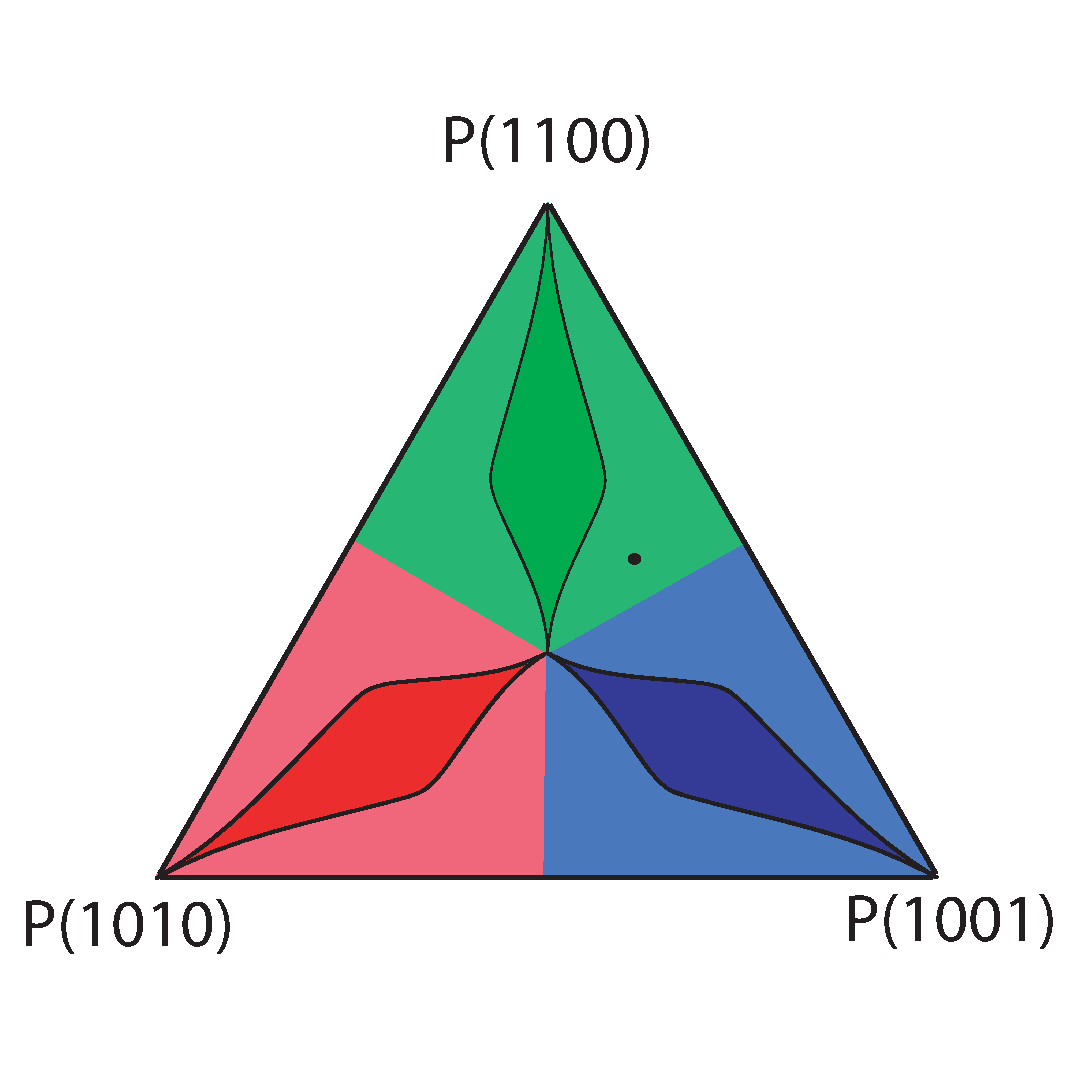
\includegraphics[width=0.48\textwidth]{../newimages/simple-treespace-sample.pdf}
    \put(-180,10){\myFigLabel{figSimpleDataCounter}: pattern frequency space}
   \vspace{-0pt}
   \vspace{-40pt}
  \end{center}
\end{wrapfigure}
I plot (Fig. \arabic{figSimpleDataCounter}) the relative frequencies of these patterns in \href{http://en.wikipedia.org/wiki/Barycentric_coordinate_system_(mathematics)}{Barycentric coordinate space}, as shown on the right.
The frequency of a pattern can be read by looking at the distance between the point and the sides of the equilateral triangle.
Somewhat confusingly the pattern frequency is the distance from the side that is opposite the labelled point.
So the point shown by the black dot would represent approximately:
\begin{eqnarray*}
	P(1100) & \approx & 0.5\\
	P(1010) & \approx & 0.1\\
	P(1001) & \approx & 0.4
\end{eqnarray*}
(remember these are the relative frequencies of the patterns given that it is parsimony-informative pattern, so these have to sum to one).

\begin{wrapfigure}{r}{0.5\textwidth}
  \begin{center}
   \vspace{-40pt}
    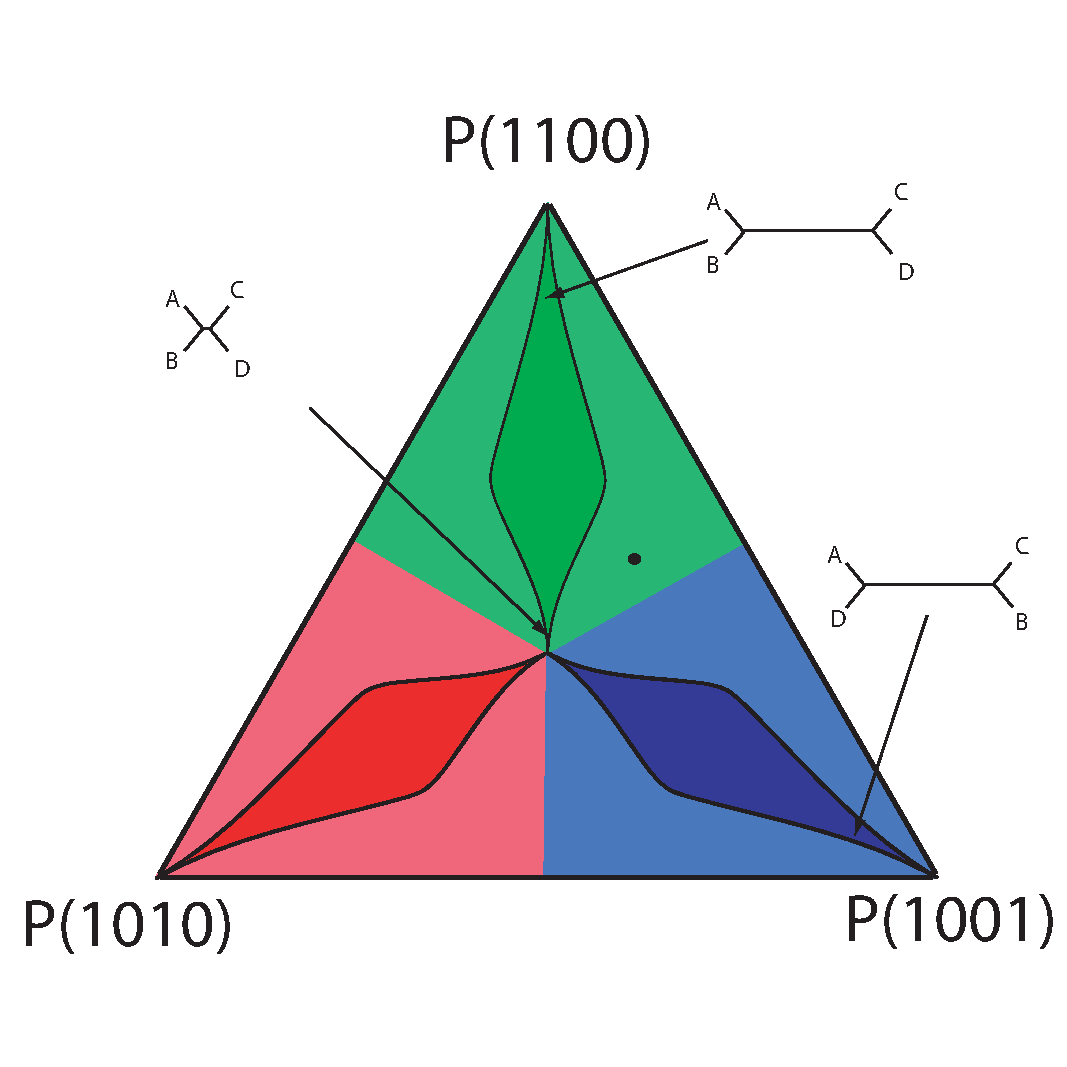
\includegraphics[width=0.48\textwidth]{../newimages/simple-treespace-trees.pdf}
    \put(-160,20){\myFigLabel{figSimpleTreeCounter}: simple trees}
   \vspace{-10pt}
    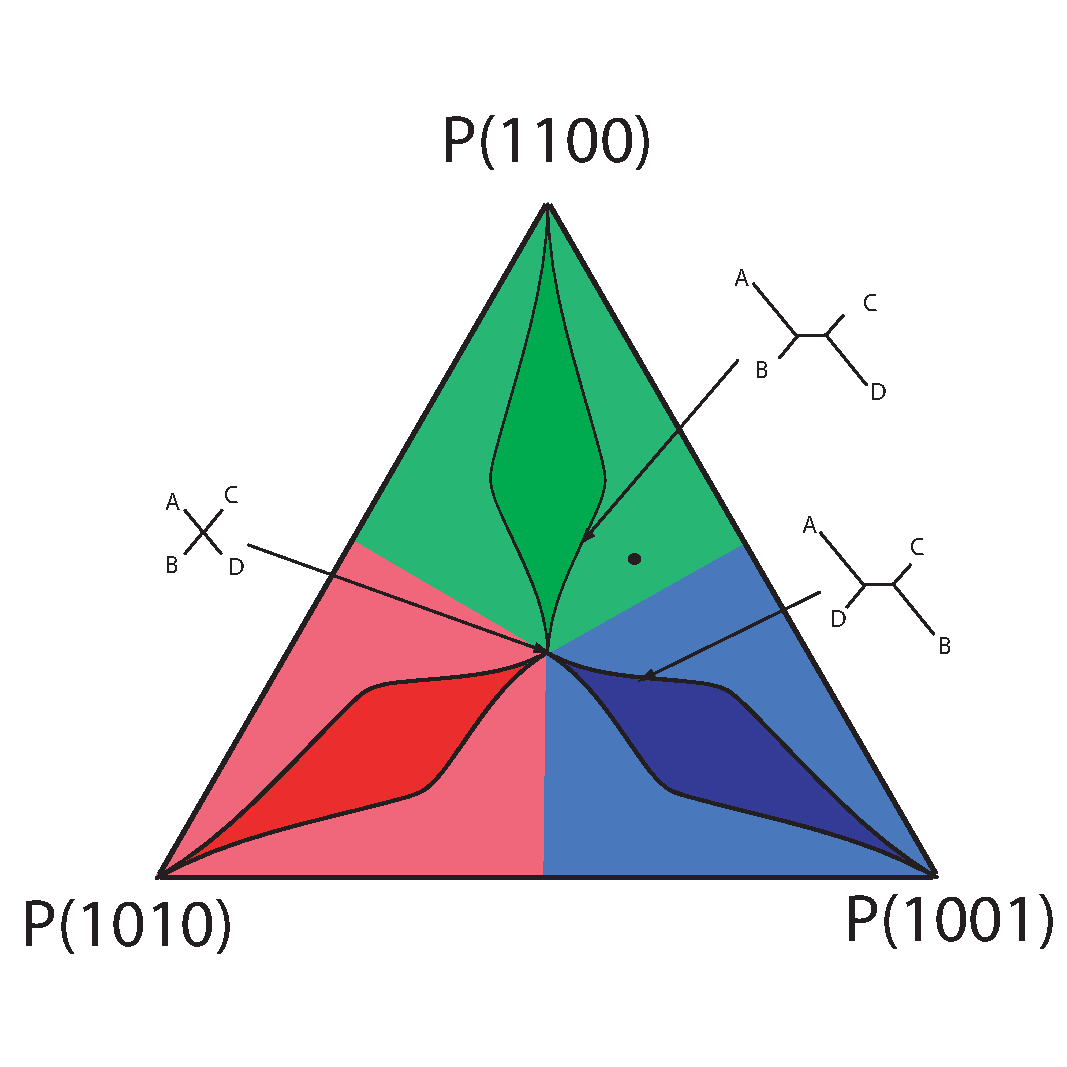
\includegraphics[width=0.48\textwidth]{../newimages/simple-treespace-trees2.pdf}
    \put(-160,20){\myFigLabel{figClosestTreeCounter}: closest trees}
    \vspace{-50pt}
  \end{center}
\end{wrapfigure}
We use this view of tree space because we can plot points that represent data matrices in this space, and we can also represent the {\em prediction} of different trees into the same space.
The figures to the right show how some trees project into this space.  
The idea is that if we were to use our simple model of 0$\leftrightarrow$1 evolution on those trees, then they would predict pattern frequencies that exactly match the point that the arrows point to.
So in Figure \arabic{figSimpleTreeCounter} all of the terminal branches have the same length. 
Thus, each tree predicts the data pattern that would support that tree (under parismony).  
If the internal branch is long, then close to 100\% of the parsimony-informative sites will be the ``expected'' type.
When the internal branch is short, the relative frequency of the pattern that supports the tree is closer to 1/3 (because sites that experience multiple substitutions on the terminal branches generate each type of pattern in equal frequencies).

In the lower panel (Fig \arabic{figClosestTreeCounter}), we see the points in the three trees (one for each topology) that are as close as possible\footnote{``As close as possible'' only applies if we constrain branch lengths in certain non-obvious ways. The topology tests and the real approaches to ML tree inference do {\bf not} make these constraints. I just impose them when making these figures to make the cartoons clearer.} to the sampled data (the black dot).
If we think of the distance as the Kullback-Leibler distance, then those distances can be thought of -1 times the $\lnL$ for any tree (smaller distance directly translates to higher $\lnL$ in the actual pattern frequency space\footnote{This connection is lost when we look at the relative pattern frequencies -- but we'll ignore that, since we are using these pictures as rough guides only. The KL-distance is better thought of as a log likelihood ratio between the ``multinomial likelihood'' \citep[{\em aka} the ``unconstrained likelihood'' of][]{Goldman1993} that represents the highest possible likelihood for any {\em i.i.d.} model and the likelihood under a tree model.}).
Note that the closest point for the A+C {\em vs} B+D tree is actually the star tree.
Under a star tree with all of the terminal branch lengths constrained to have same length, all three parsimony-informative data patterns will be equally frequent; thus we get a point in the center of the triangle (distance = 1/3 from each side).


\newpage
\section*{Dataset background}
I took 3000 sites from an alignment of 5 primates.

$T_1$ = (((chimp, gorilla), human),orang,gibbon), and $\ln L(T_1|X) = -7363.296$\par
$T_2$ = (((chimp, human), gorilla),orang,gibbon), and $\ln L(T_2|X) = -7361.707$\par

Below is a depiction of the $\delta$ test statistic and the expected value of the test statistic if we believe that the trees are equally good.\par
\begin{picture}(0,50)(0,-50)
	  \put(110,0){\small$\delta(T_1,T_2|X)=-3.18$}
	  \put(270,0){\small$\mathbb{E}(\delta) = 0$}
	  \put(130,180){\makebox(0,-190)[l]{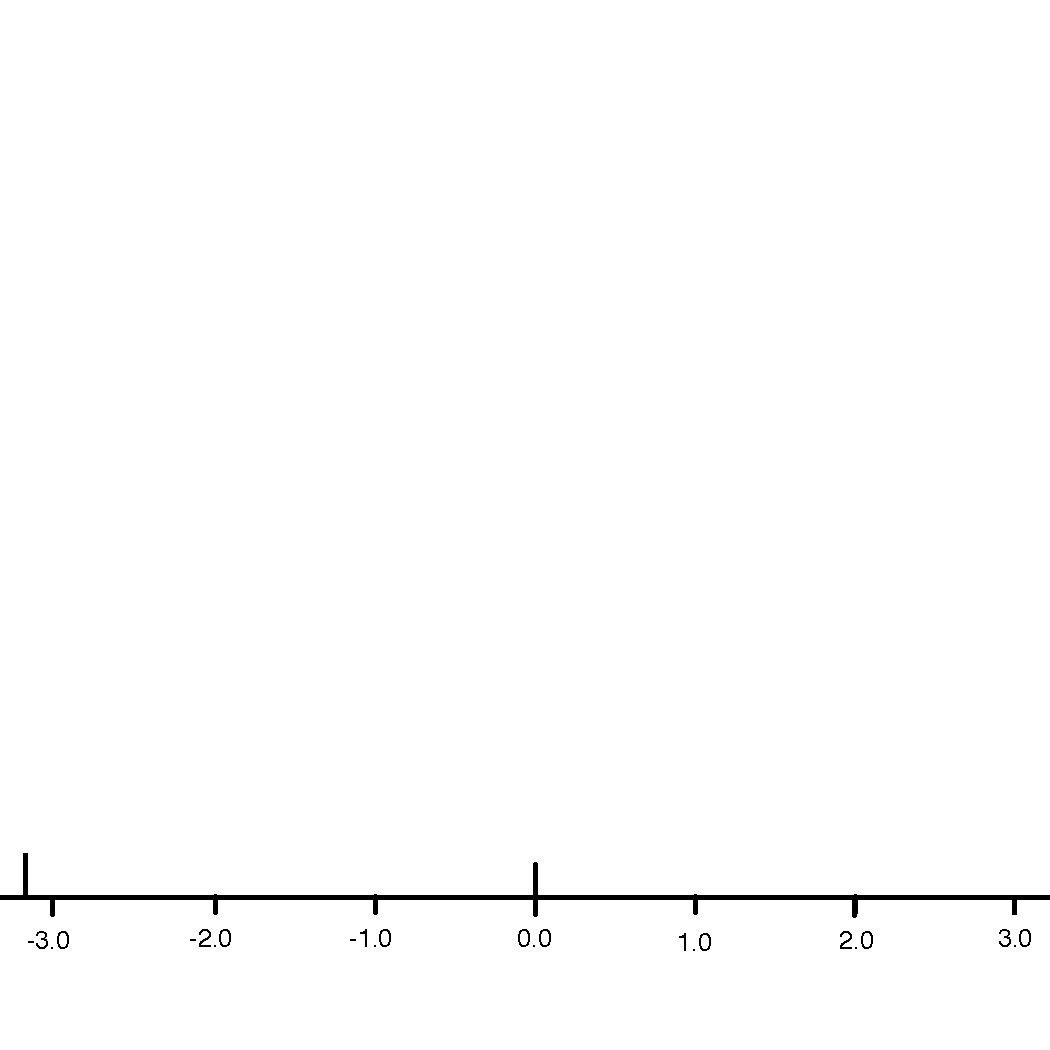
\includegraphics[scale=.6]{../newimages/delta_axes.pdf}}}
	  \put(250,-60){$\delta(T_1,T_2|X) $}
\end{picture}

To get a sense of the variability in the signal, we can look like the $\delta$ statistic calculated on each site:\\
\begin{picture}(500,280)(0,-280)
	  \put(40,-120){\makebox(0,0)[l]{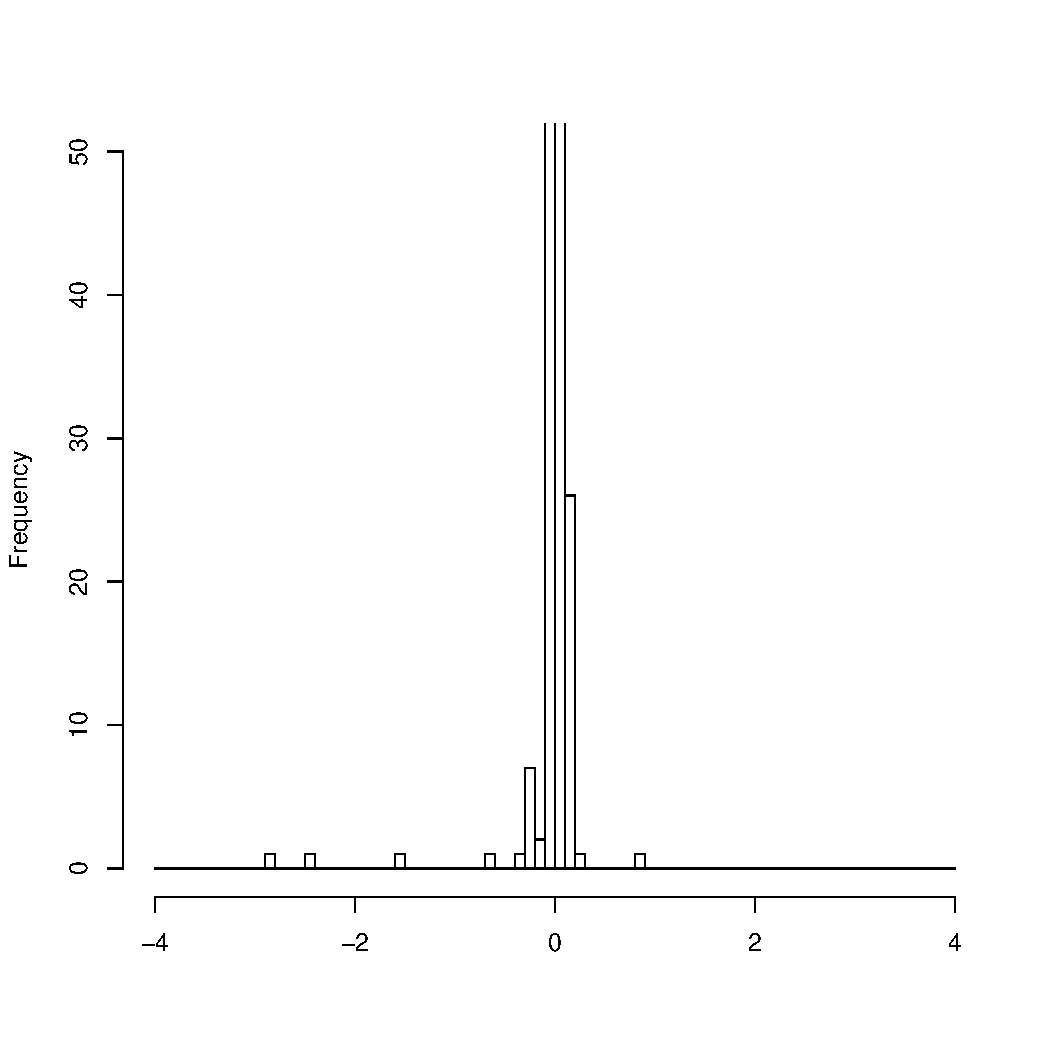
\includegraphics[scale=0.6]{../scripts/mtdna/d1-2hist.pdf}}}
	  \put(170,-260){\normalsize$\delta(T_1,T_2|x_i)$}
	  \put(40,-120){\makebox(0,0)[l]{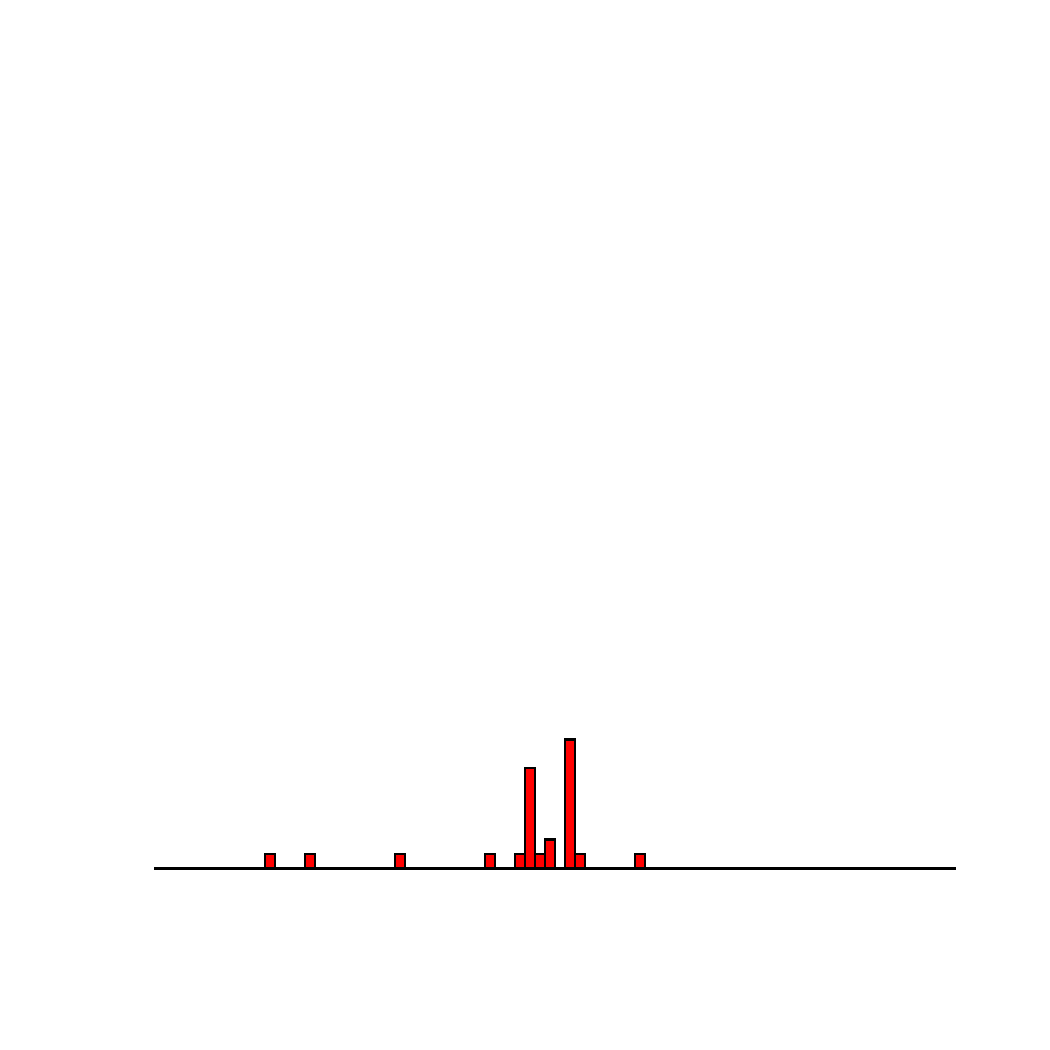
\includegraphics[scale=0.6]{../scripts/mtdna/diff1-2hist.pdf}}}
	  \put(300, -50){\myFigLabel{figSiteDeltaCounter}: histogram of per site $\delta$ statistics}
\end{picture}
Note that the central bars of this histogram are cropped -- almost all of the sites do not discriminate strongly between these trees so that $\delta(T_1,T_2|x_i)\approx0$ for these sites.
The per site $\delta$ statistic for the 26 sites which have different parsimony scores on the two trees are shown in red.
Also note that the notation uses $x_i$ indicating that we are calculating the likelihood for a site (a subscript on $x$ will indicate a site index).  

\subsubsection{A side note on the Templeton test} In case you are curious, $\delta(T_1,T_2|x_i)\approx0$ instead of $\delta(T_1,T_2|x_i)=0$ even if a site $i$ represents a constant pattern.
You may wonder how a constant pattern prefers one tree over another tree.
The short answer is that a constant pattern by itself will not prefer one topology over another, but in the process of maximizing the likelihood jointly over all parameters the two trees will predict different probabilities of even the constant patterns.
Typically (if we ignore the numerical parameters of the model of sequence evolution), we will find that the smaller tree (the tree with the smaller sum of branch lengths) will predict more constant patterns.
This makes sense, because there is less opportunity for change on small trees.
Thus, even constant patterns will discriminate {\em very} slightly between trees.
The Wilcoxon signed-rank test (that goes by the name of ``Templeton test'' in the realm of phylogenetics \citep{Templeton1983}) ignores the precise degree of preference for a tree, and simply ranks the sites by their preference between trees.
The test was proposed as a means of assessing statistical support when using parsimony, but has been applied to likelihood differences as well.
Because the subtle interactions between data and parameters lead to unexpected effects (such as constant patterns all favoring one tree, but very slightly), this sort of ranking of sites may not be a wise approach when using ML phylogenetic techniques.
The ``Paired-sites tests'' chapter (Chapter 21) of \citep{Felsenstein2004} discusses these issues more thoroughly.


\newpage
\section*{KH Test \citep{KishinoH1989} }
Two trees, $T_1$ and $T_2$, must be chosen {\bf before} looking at the data at hand.

\subsubsection{Test statistic} $\delta(T_1,T_2|X)$

\subsubsection{Null hypothesis} Two trees will explain the data equally well. 
In notation $\expect{\lnL(T_1|X)} = \expect{\lnL(T_1|X)}$ (where $\expectation$ denotes the expected value).  Thus:
$$\expect{\delta(T_1,T_2|X)} = 0$$

\subsubsection{Null distribution} We use the null hypothesis to let us set the expected value of the null distribution to 0.
To finish specifying the null distribution we can either
\begin{compactenum}
	\item Assume the the $\lnL$ values will follow a Normal distribution, and estimated the variance. Or
	\item Use bootstrapping to generate the a distribution, and then ``center'' this distribution so that it fits our null assumption that the mean of the distribution will be 0.
\end{compactenum}

\subsubsection{Details of the bootstrapping approach}
A distribution of $\delta(T_1,T_2|X^{(\ast)})$ values is created by bootstrapping the data and recalculating the likelihood score on each tree (often this is done through the RELL procedure).
An example for the primate dataset is shown below (before centering on the left and centered on the right).
Note that the mean of this distribution, $\bar{\delta}(T_1,T_2|X^{(\ast)})$, taken over bootstrap replicates is very close to the observed value of the test statistic (around -3.2).\\
\begin{picture}(500,280)(0,-280)
	  \put(-30,-120){\makebox(0,0)[l]{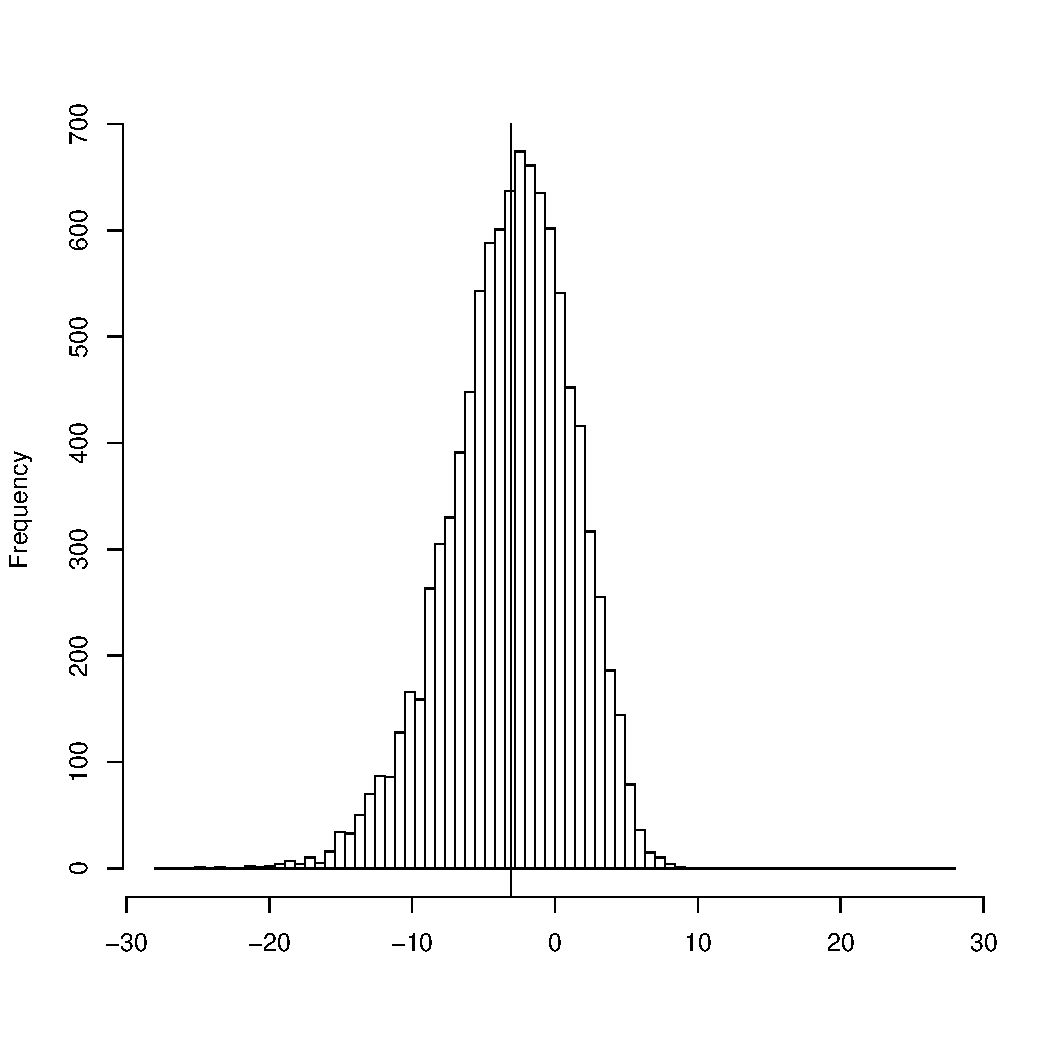
\includegraphics[scale=0.5]{../scripts/mtdna/uncentered1-2hist.pdf}}}
	  \put(70,-260){\normalsize${\delta}(T_1,T_2|X^{(\ast)})$}
	  \put(230,-120){\makebox(0,0)[l]{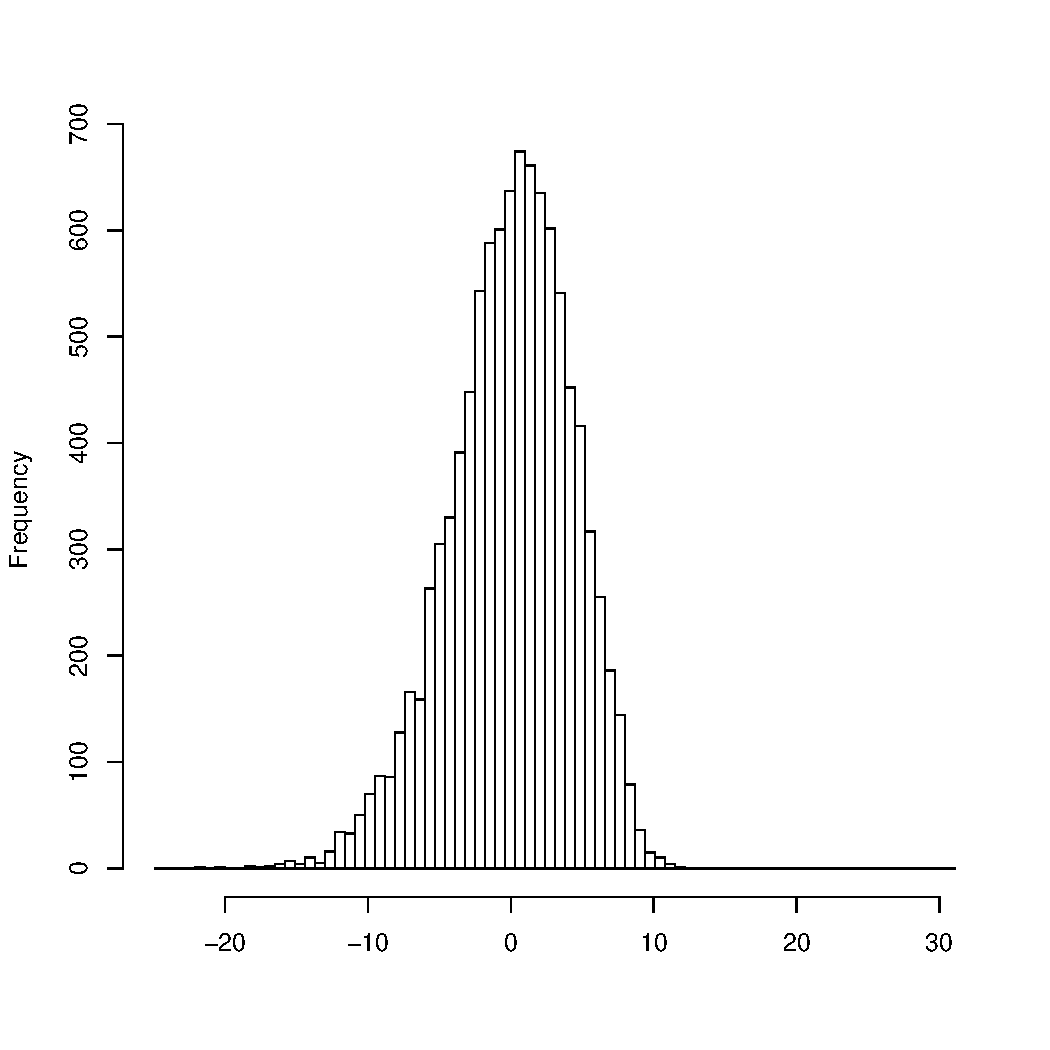
\includegraphics[scale=0.5]{../scripts/mtdna/centered1-2hist.pdf}}}
	  \put(280,-260){\normalsize${\delta}(T_1,T_2|X^{(\ast)}) - \bar{\delta}(T_1,T_2|X^{(\ast)})$}
\end{picture}

Subtracting the mean of the bootstraps is a very simple procedure, but it is justified by the fact that expected value should be 0 under the null and the fact that the mean of a large sample should be close to the expected value.
We then treat the centered distribution as a simulation of draws from the null distribution.
We can calculate a \pvalue by counting the proportion of replicates from this simulated null yield values that deviate from the null at least as strongly as the observed test statistic (\pvalue$\approx$ 0.48 in this example).
In the figure below the tail region are shown in red.
Artifacts caused by binning values in the histogram make it appear that some of the values are less extreme than the observed value, but this is not the case.\\
\begin{picture}(500,280)(0,-280)
	  \put(100,-120){\makebox(0,0)[l]{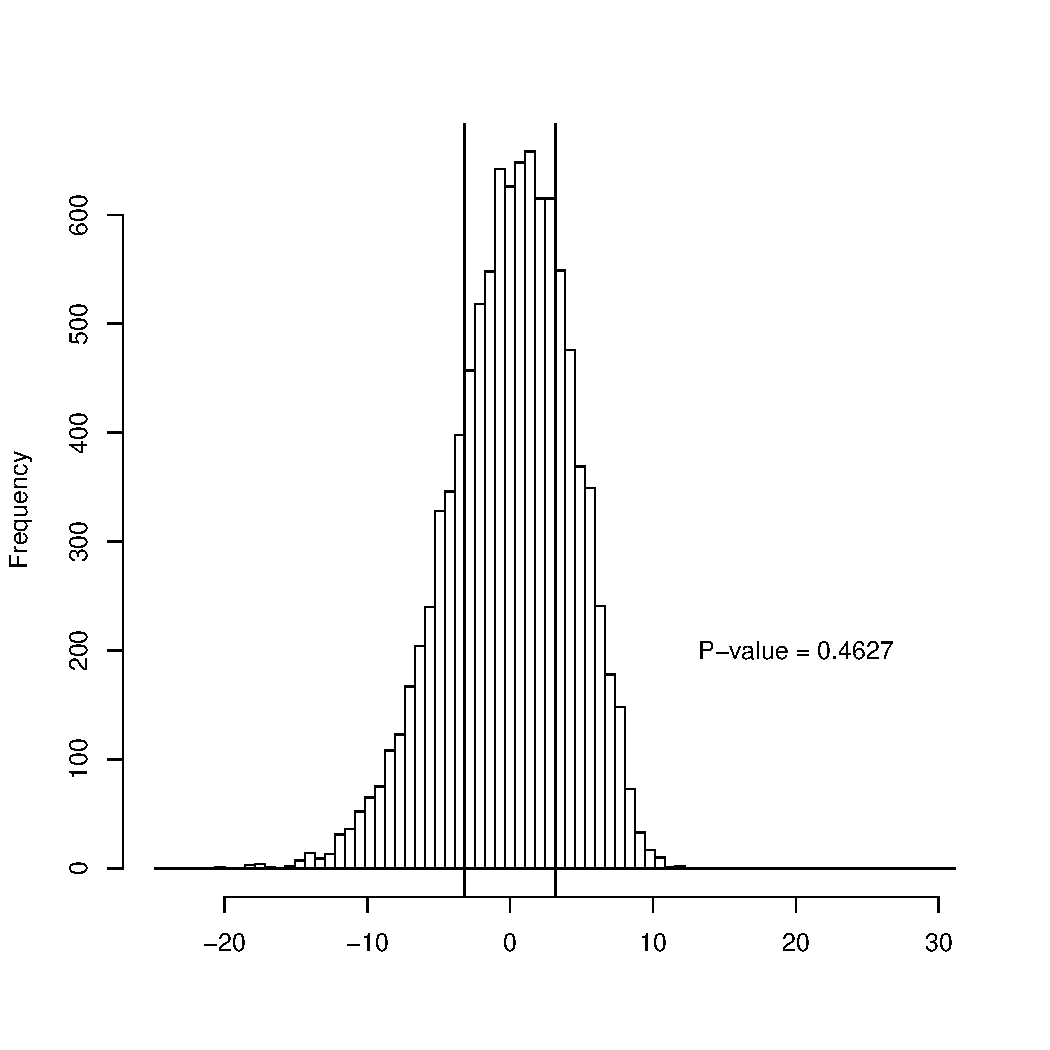
\includegraphics[scale=0.5]{../scripts/mtdna/centered1-2hist-p.pdf}}}
	  \put(100,-120){\makebox(0,0)[l]{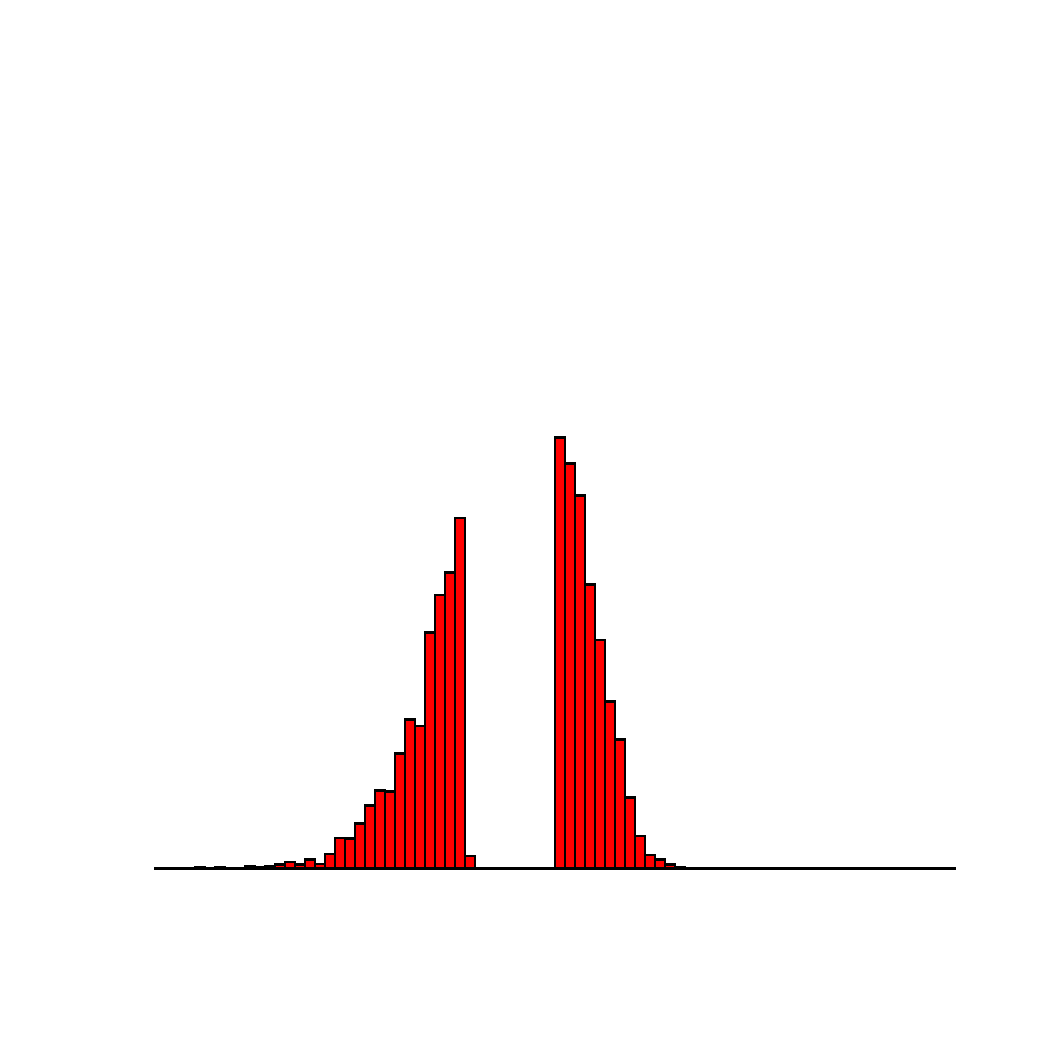
\includegraphics[scale=0.5]{../scripts/mtdna/centered1-2hist-tails.pdf}}}
	  \put(180,-260){\normalsize${\delta}(T_1,T_2|X^{(\ast)}) - \bar{\delta}(T_1,T_2|X^{(\ast)})$}
\end{picture}
You would have to do an enormous number of simulations if you wanted to estimate the \pvalue with great precision, but 10,000 RELL bootstraps do not take much computational effort.

\begin{wrapfigure}{r}{0.5\textwidth}
  \begin{center}
   \vspace{0pt}
    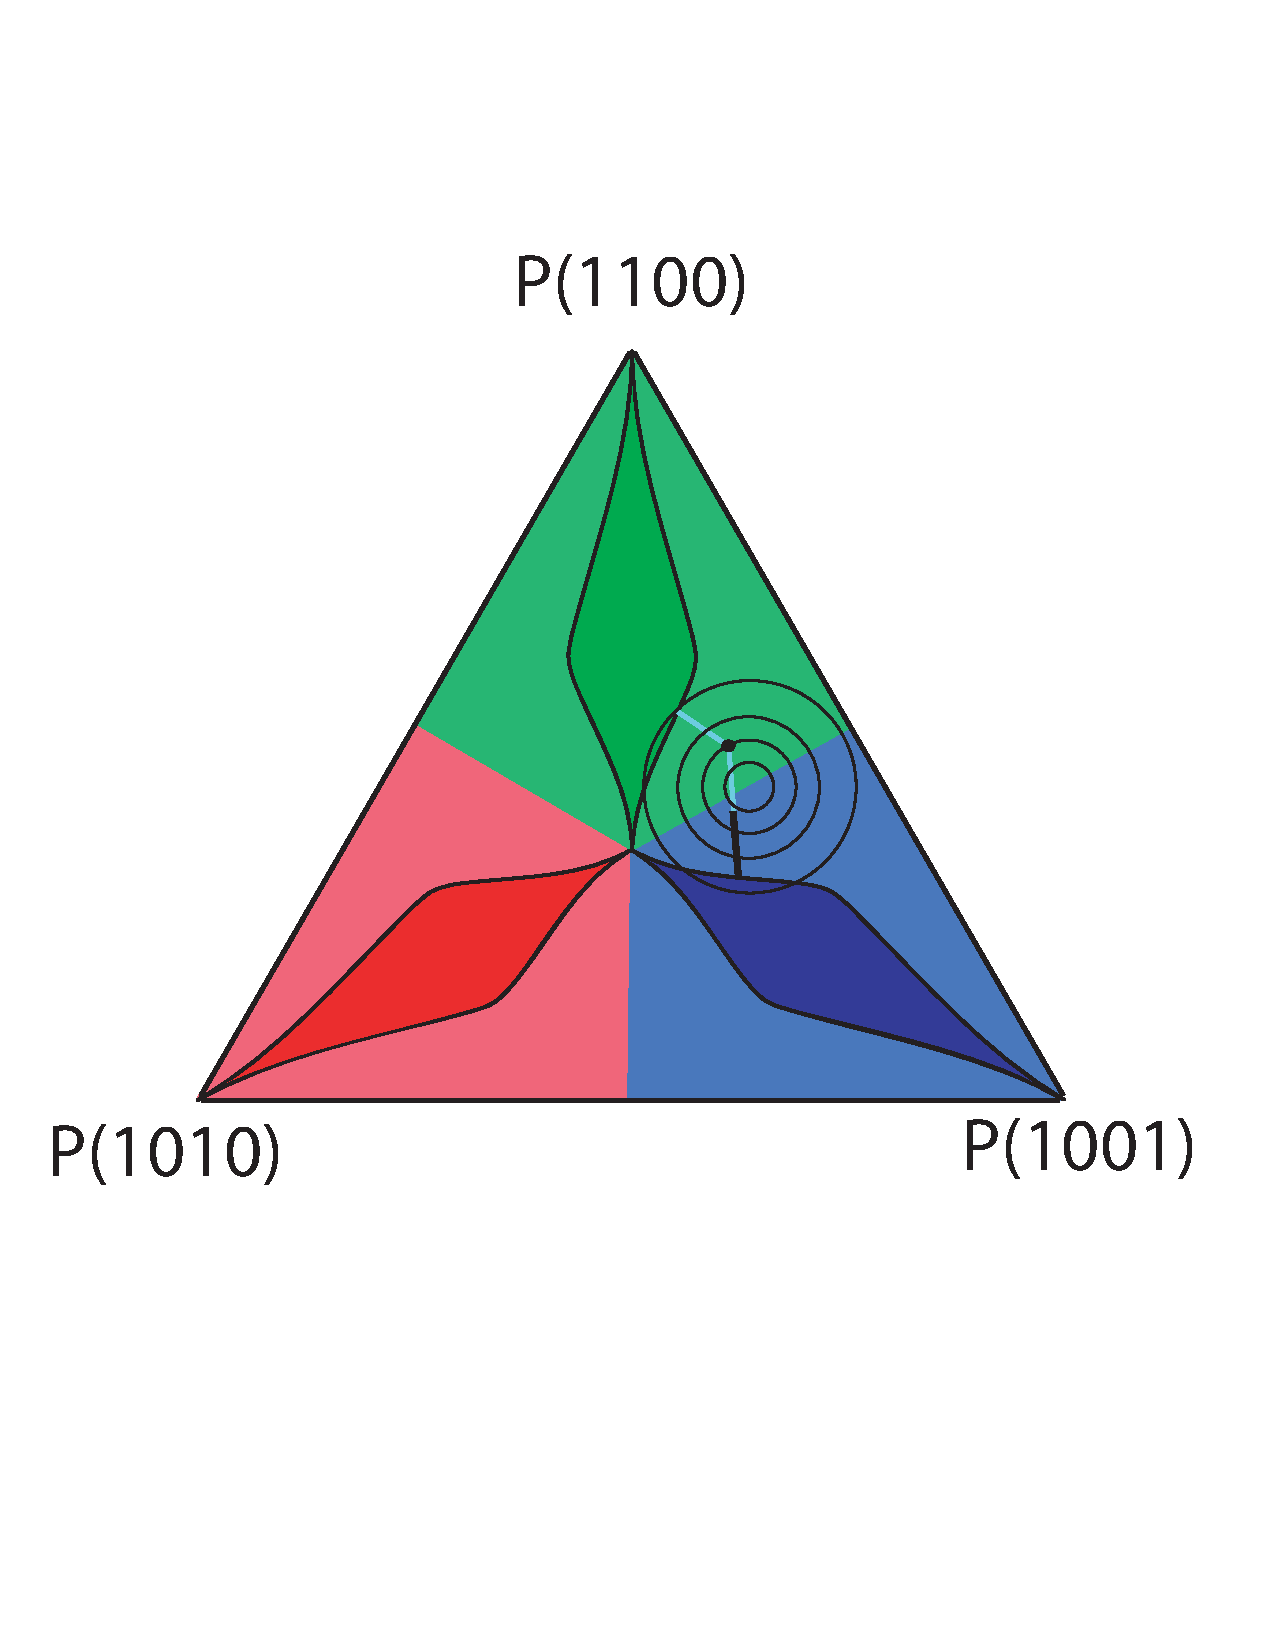
\includegraphics[width=0.48\textwidth]{../newimages/simple-treespace-kh.pdf}
    \vspace{-120pt}
    \put(-160,70){KH Test Cartoon shown in lecture}
  \end{center}
\end{wrapfigure}
We can depict the KH Test in a cartoon of pattern frequency space as shown to the right.
The intent of the cartoon is to display the test statistic with lines connecting the
ML estimates of branch lengths in the tree to the point that corresponds to the pattern frequencies in the observed data (shown as a black dot). 
The length of the lines is negatively related to the $\lnL$, and the black portion is intended to convey the difference in the $\lnL$ between the trees; this is our $\delta$ test statistic.
In this cartoon, we can view the patterns as being ordered `chimp', `human', `orang+gibbon', and `gorilla'
Thus the tree with the highest likelihood, $T_2$, is colored in green and depicted with the 1100 pattern (chimp+human), and the other {\em a priori} tree, $T_1$, unites chimp and gorilla (pattern 1001).

The contour lines centered around the boundary between hypotheses are intended to convey the fact that we generate the null distribution by bootstrapping to create a population points in pattern frequency space (the contours can be thought of as a contours of the probability distribution, with the highest probability region being the central circle).
Recall that in the KH test, we calculate the $\delta$ test statistic for each bootstrapped replicate and then we center these values on 0; this centering is the reason that the contours in the KH test cartoon are centered on the boundary between $T_1$ and $T_2$.
In the actual test the $\delta$ test-statistics are ``centered'' to have a mean of 0, so perhaps the cartoon should look like the one below (note it is really the $\delta$ test statistics that are being centered, not the bootstrapped points in pattern frequency space; but I still find these figures helpful).
\begin{picture}(500,300)(0,-300)
	  \put(-70,-120){\makebox(0,0)[l]{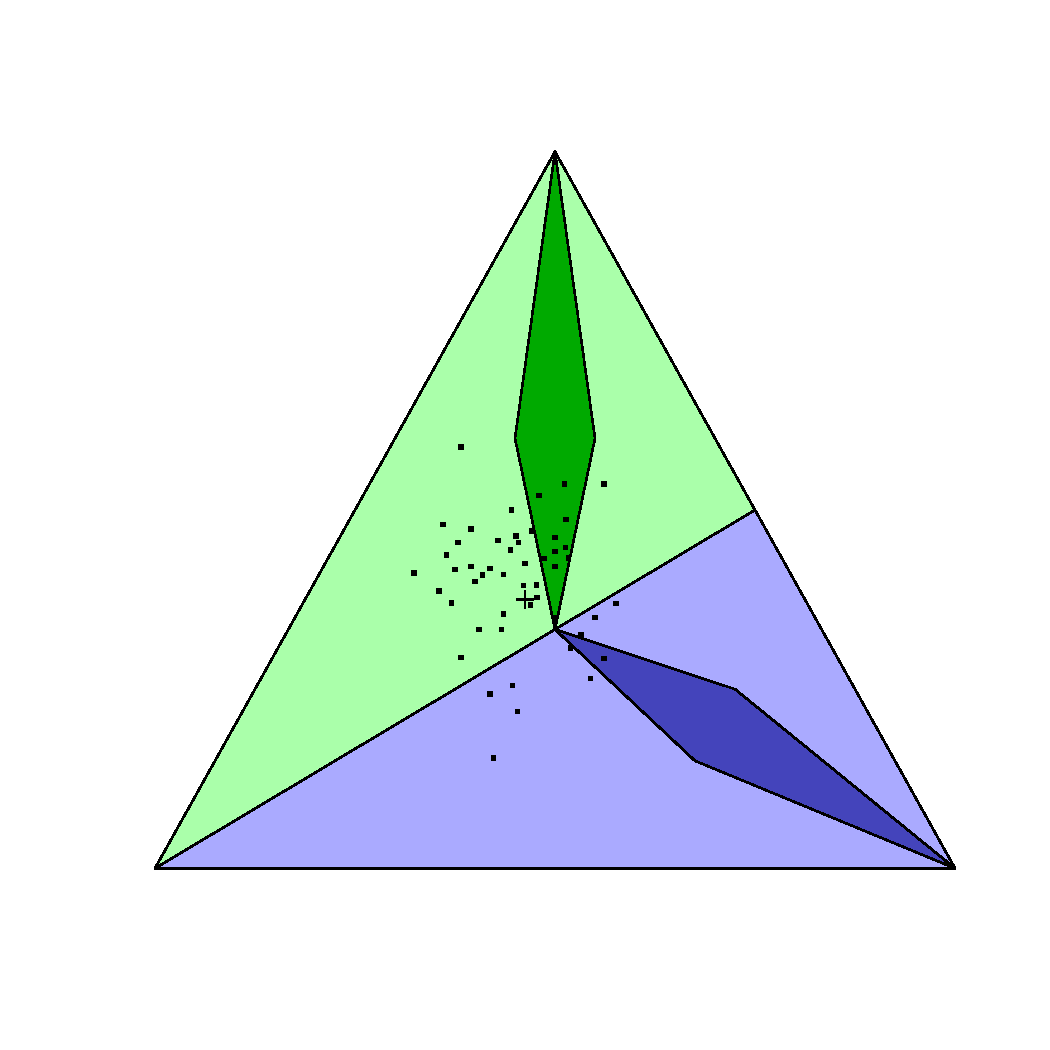
\includegraphics[scale=0.4]{../scripts/mtdna/kh_points_before.pdf}}}
	  \put(130,-120){\makebox(0,0)[l]{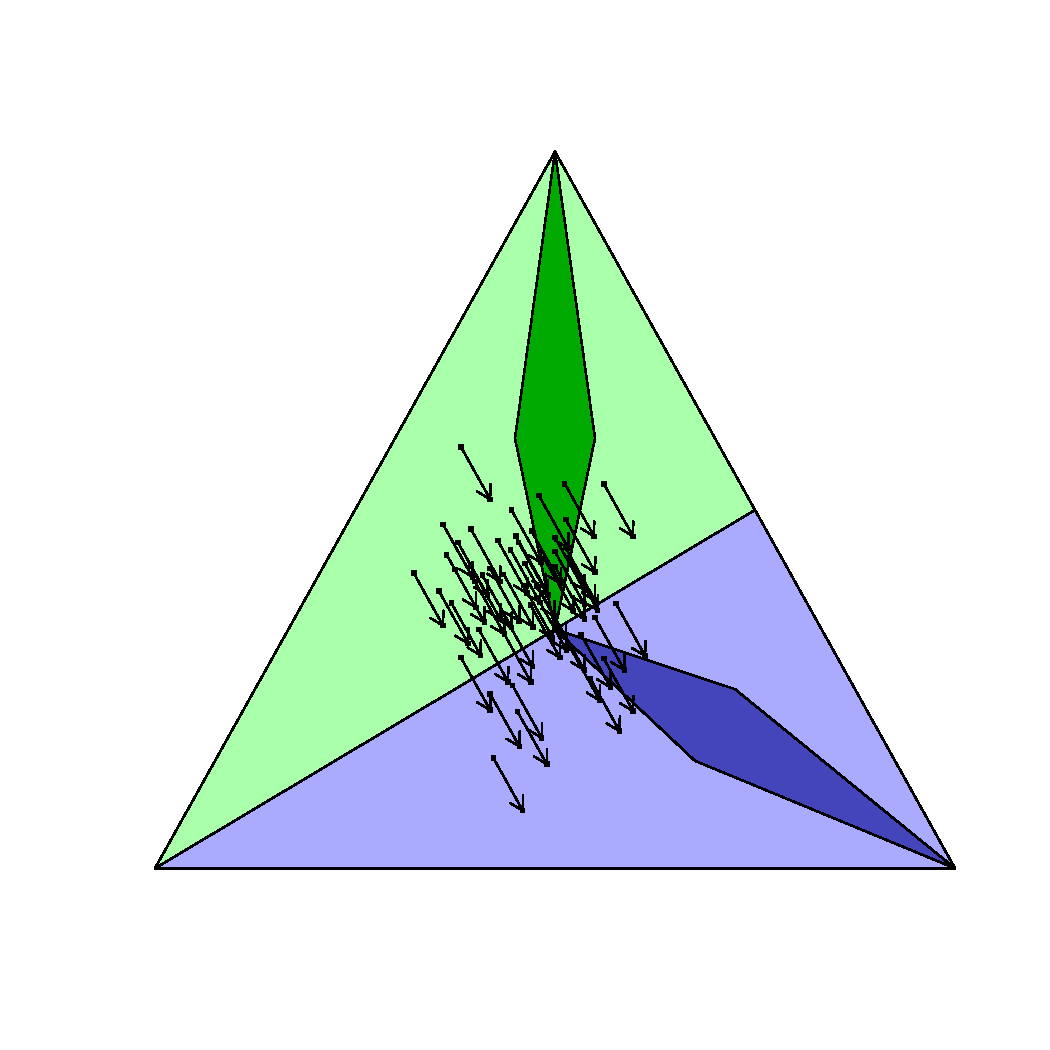
\includegraphics[scale=0.4]{../scripts/mtdna/kh_points_arrows.pdf}}}
	  \put(330,-120){\makebox(0,0)[l]{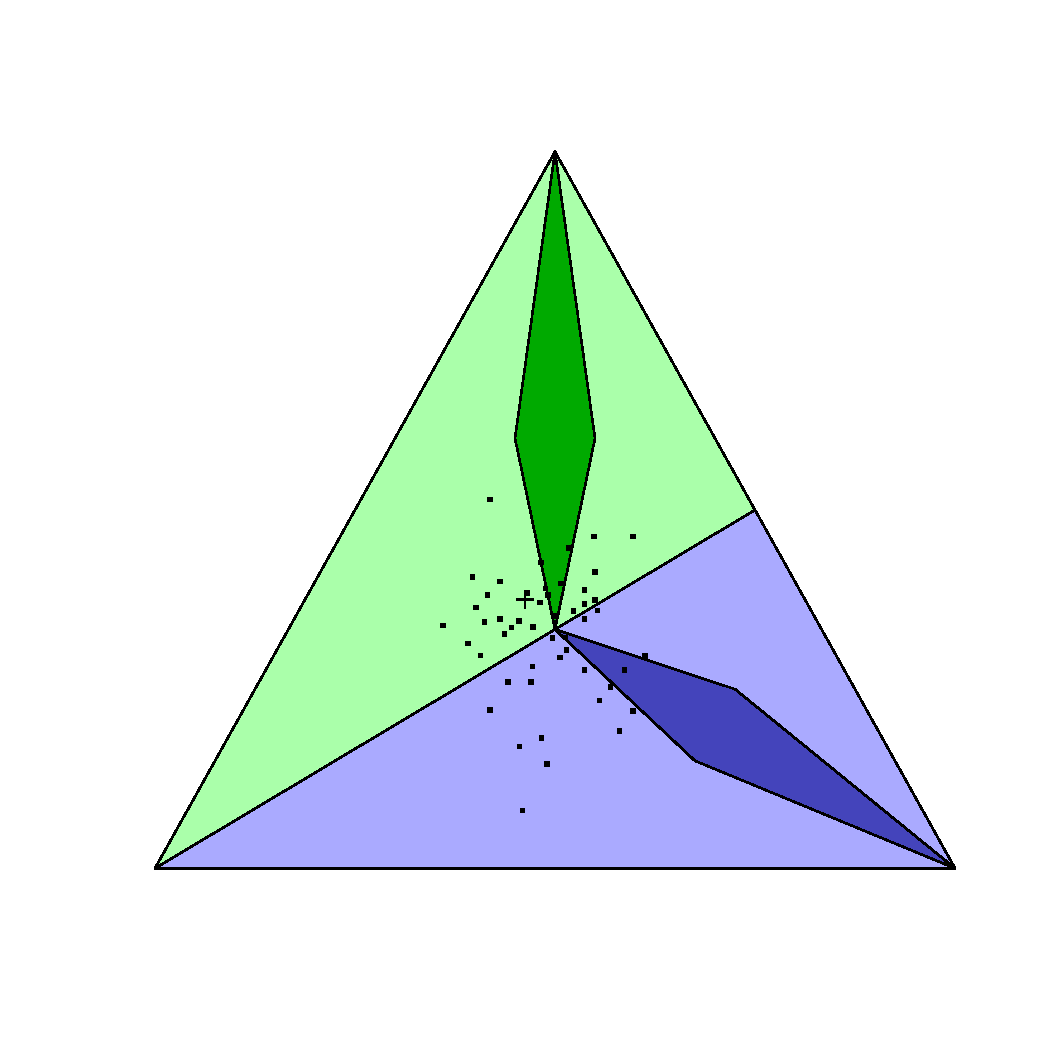
\includegraphics[scale=0.4]{../scripts/mtdna/kh_points_after.pdf}}}
	  \put(-40,-210){\normalsize Observed data ($+$ sign), and }
	  \put(-40,-222){\normalsize bootstrap pseudoreplicates (black) }
	  \put(160,-210){\normalsize Center each the $\delta$ from each  }
	  \put(160,-222){\normalsize  bootstrap, such that the mean is 0 }
	  \put(360,-210){\normalsize After centering. The observed $\delta$ }
	  \put(360,-222){\normalsize (corresponding to the data point }
	  \put(360,-234){\normalsize denoted by $+$ sign) is {\em not}}
	  \put(360,-246){\normalsize ``centered.'' Instead we use the}
	  \put(360,-258){\normalsize centered bootstrap reps of $\delta$ to}
	  \put(360,-270){\normalsize calculate a \pvalue: what is the }
	  \put(360,-282){\normalsize probability that a value as extreme }
	  \put(360,-294){\normalsize as $+$ would arise under the null. }
    \vspace{10pt}
\end{picture}

In these figures only 2 trees are considered. 
The ``red'' tree depicted in other views of pattern frequency space is not shown.
This is done because the KH test requires that two trees be specified {\em a priori}.  
It is {\em not} appropriate to use this test to reject one {\em a priori} tree by comparing it to the ML tree.

\subsection{Performing the KH test in PAUP}
Assuming that you have chosen an appropriate model of sequence evolution (and configured PAUP to use that model using the {\tt LSet} command, then the KH test can be run by the commands:
\begin{verbatim}
GetTrees file = tree1.tre mode = 3 ;
GetTrees file = tree2.tre mode = 7 ;
LScore / KHTest=RELL ;
\end{verbatim}
Note that you can use the command {\tt LScore / KHTest=FullOpt } to maximize the likelihood on each bootstrap replicate, $j$, when calculating $\delta\left(T_1,T_2|X^{(j)}\right)$, but that is rarely computationally feasible.

\subsection{Normal approximation versions of the KH test} 
Because the total $\delta$ is a sum over all sites: $$\delta\left(T_1,T_2|X\right) = \sum_{i=1}^M\delta\left(T_1,T_2|x_i\right),$$
the Central Limit Theorem implies that we should be able to use the Normal distribution as our null distribution.
This is a large sample property, and it may not hold for even fairly big datasets.  
For instance in the case of the primate dataset that we are considering, the per site $\delta$ test statistics are skewed to the left; and the bootstrapping approach reveals that this skew shows up in the distribution of $\delta\left(T_1,T_2|X^{\ast}\right)$ for the bootstrap replicates.
The Central Limit Theorem, guarantees that this skew will eventually go away as we move to larger datasets; and the Normal distribution will be a good surrogate for the null distribution in these cases.

The number of sites that we are summing across is large (3000), but the vast majority show $\delta$ values of very close to 0.  
Only 40 strongly discriminate between trees.  
The very ``fat-tailed'' distribution of per site $\delta$ values means that convergence of the sum to a normal will require a very large sample of sites.

If we do feel comfortable making the assumption that the null distribution is a Normal we can use the mean$=0$ and variance $M$ times the variance of $\delta$ across all sites.
The mean of 0 comes from the assumption of our null.
The variance comes from the fact that the variance of a sum is the sum of the variances:
$$ \sigma_{\delta\left(T_1,T_2|X\right)}^2 = \sum_i^M\sigma_{\left(T_1,T_2|x_i\right)}^2 = M\sigma_{\left(T_1,T_2|x\right)}^2$$
(where the last equality comes from assuming that the sites are {\em i.i.d.} so the have their $\delta$ statistics are drawn from a distribution with the same variance for each site; so we can drop the $i$ subscript for each site).

\subsubsection{Using the normal approximation in PAUP} Substituting the command {\tt LScore / KHTest=Normal }	 will tell PAUP to use the normal approximation.
In the example of this data set, the results are quite different.
The RELL approach gives a $P \approx 0.48$, while assuming a Normal strongly rejects the chimp+gorilla tree $P < 0.001$.
I would trust the RELL approach in this case.

As discussed in \citet{GoldmanAR2000}, PAUP makes the stringent assumption that the per site $\delta$ values (not just the $\delta\left(T_1,T_2|X\right)$ statistic) follows a Normal.

\subsection{Summary of the KH Test} This test is appropriate when you have two trees specified {\em a priori} that you want to test with a new dataset. 
The $\delta$ test-statistic is very powerful, but the test is non-parametric because it uses only mild assumptions to determine the null distribution of the test statistic. 
Specifically, we use the fact that the null states that the expected value of $\delta$ is 0, and we use the nonparametric approaches to estimate the variance of the null distribution.
Thus the KH Test should be fairly robust to model violation ({\em e.g.}~using an oversimplified model to score trees).

\newpage
\section*{SH Test \citep{ShimodairaH1999}}
As discussed by \citet{GoldmanAR2000} the KH Test should not be used when you have one tree specified {\em a priori} and you would like to test the ML tree against this tree.
Because you are searching through tree space to find the ML tree, using a KH Test will suffer from ``selection bias'' in which the selection of the optimal tree biases the test statistic to large values.
In other words, even under a null hypothesis that $T_1$ will explain the data as well as another tree, you would expect large values of $\delta(\hat{T}, T_1|X)$ to arise simply because $\hat{T}$ is selected on the basis of having a high ML score.

The SH test corrects for selection bias, by requiring the investigator to designate a set of candidate trees. 
This set could be the set of all possible trees.

\subsubsection{Test statistic} $\delta(\hat{T},T_i|X)$ for any tree, $T_i$, in your candidate set.

\subsubsection{Null hypothesis} For each tree, $T_i$, in your candidate set you expect to explain the data as well as any other tree in the candidate set (if you have no sampling error).

\subsubsection{Null distribution} Unlike in the KH Test, we {\em cannot} assume that $\delta(\hat{T},T_i|X)$ is centered around 0.
In fact $\delta(\hat{T},T_i|X)$ will be positive for every tree that is not the MLE tree (if $T_i$ is tied for being the ML tree, then  $\delta(\hat{T},T_i|X) = 0$).
If a statistic is always positive or zero, then its expectation cannot be 0.
We must account for the fact that we are testing a large number of trees against the tree that appears to be the best explanation of  the data.

Our approximation of the null distribution will rely on the fact that our expectation is that all of the trees in candidate set will explain the data equally well.
In notation, $A = \expect{\lnL(T_i|X)}$, where $A$ is the (unknown) expected likelihood of each tree in the candidate set.
We do not need to know what value $A$ has.
Because our test statistic is the difference in $\lnL$ values, it is only important to note that the expected $\lnL$ is the {\em same} for all trees in the candidate set.

In the SH test, we bootstrap to get a sense of the variability of $\lnL$ scores as a result of sampling error.
But rather than ``centering'' $\delta\left(\hat T,T_i|X^{\ast}\right)$ around 0,  we center each tree's distribution of $\lnL$ scores around 0 (we could choose any number to center the distributions around, but 0 is convenient).
So for each tree we center the distribution of $\lnL\left(T_i|X^{\ast}\right)$ by subtracting the mean, $\bar{\lnL}\left(T_i|X^{\ast}\right)$, for that tree over all bootstraps replicates.

To calculate the null distribution of the test statistic, we then look at the magnitude of the differences between a bootstrap replicate's ``centered'' $\lnL$ and the largest ``centered'' $\lnL$ over all trees.
Using this difference from the largest value mimics the ``selection bias'' that is introduced by choosing to compare all of the trees to the best tree on the dataset at hand.

Thus, after bootstrapping and centering we obtain, for each tree, a distribution of centered $\delta$ values. 
This distribution describes how large we would expect $\delta$ to be even if all of the trees had the same expected score -- all of the centered $\delta$ values arise from sampling error (due to the fact that we have a finite sample of sites) and the selection bias of comparing trees to the best tree.

\subsubsection{Details of the bootstrapping approach}
A more algorithmic description of the bootstrapping procedure would be:
\begin{enumerate}
	\item For each tree $T_i$ in the candidate set calculate $\delta(\hat{T}, T_i|X)$. This is the observed value of the test statistic for each tree.
	\item Bootstrap to generate ${\ln L}(T_i|X^{(j)})$ for each bootstrap replicate $j$.
	\item For each tree $T_i$, use the mean, $\bar{\ln L}(T_i|X^{\ast})$, over all bootstrap replicates to center the bootstrapped collection of log-likelihoods:
		$$c_i^{(j)} = {\ln L}(T_i|X^{(j)})-\bar{\ln L}(T_i|X^{\ast})$$
	\item For each bootstrap replicate, $j$, pick the highest value from the centered distributions (this mimics the selection bias): $$m^{(j)} = \max\left[c_i^{(j)}\right] \mbox{ over all } i$$
	\item Then for each tree and replicate, you get a sample from the null $\delta_i^{(j)} = m^{(j)} - c_i^{(j)}$
	\item $P$-value for tree $T_i$ can be approximated by seeing where in the distribution of $\delta_i^{(j)}$ values it lies. The $P$-value is the proportion of bootstrap replicates for which $$\delta_i^{(j)} \geq \delta(\hat{T}, T_i|X)$$
	\item Trees in the candidate set with low \pvalues can be rejected; the remaining trees represent your confidence set of trees.
\end{enumerate}

\subsubsection{SH Test on the primate dataset}
Suppose that we were interested in the relationships among human, chimp, and gorilla; but we were unwilling to entertain the possibility that these three were not a monophyletic group.
In this case we would have 3 candidate trees:\\
{\color{blue} $T_1$} = (((chimp, gorilla), human),orang,gibbon), and $\ln L(T_1|X) = -7363.296$\\
{\color{green} $T_2$} = (((chimp, human), gorilla),orang,gibbon), and $\ln L(T_2|X) = -7361.707$\\
{\color{red} $T_3$} = (((gorilla, human), chimp),orang,gibbon), and $\ln L(T_3|X) = -7362.609$\\
So $T_2$ is the ML tree, and the set of $\delta$ test statistics would be\par
\begin{picture}(0,50)(0,-50)
	  \put(160,0){\tiny$\delta(\hat{T},T_2|X)=0$}
	  \put(240,0){\tiny$\delta(\hat{T},T_3|X)\approx1.8$}
	  \put(320,0){\tiny$\delta(\hat{T},T_1|X)\approx3.18$}
	  \put(30,180){\makebox(0,-190)[l]{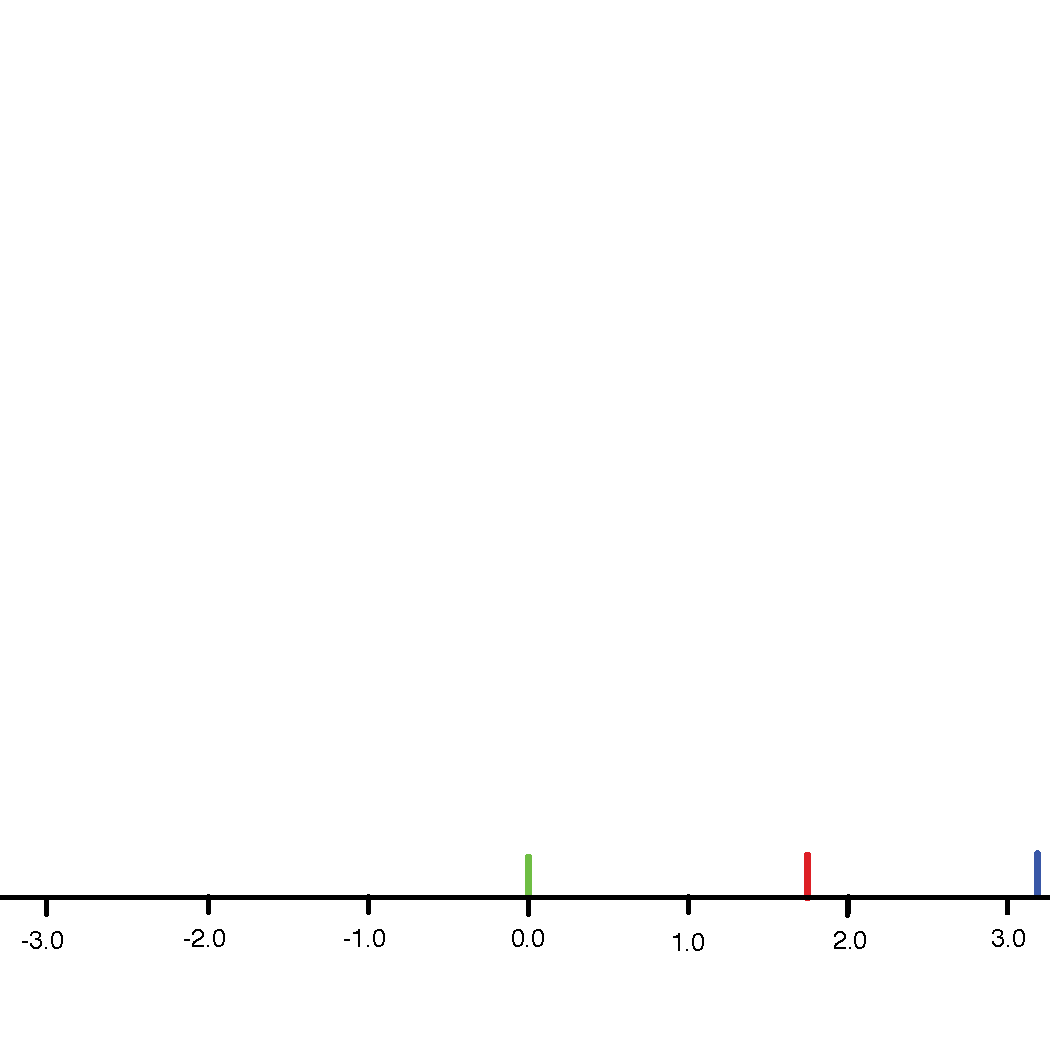
\includegraphics[scale=.6]{../newimages/delta_axes_pos.pdf}}}
	  \put(150,-60){$\delta(\hat{T},T_i|X) $}
\end{picture}


\begin{wrapfigure}{r}{0.5\textwidth}
  \begin{center}
   \vspace{-40pt}
    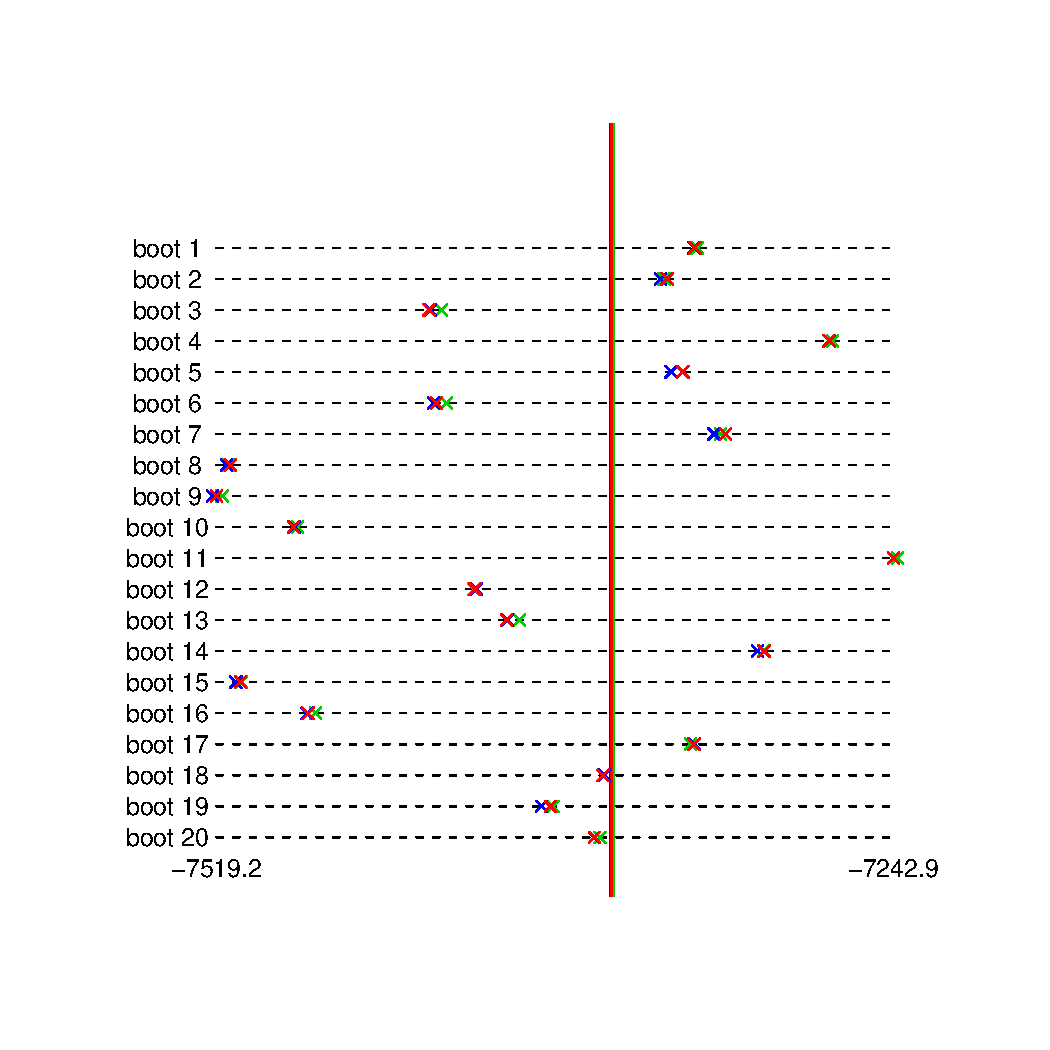
\includegraphics[width=0.48\textwidth]{../newimages/sh_test_uncentered_plots3.pdf}
    \put(-200,10){\myFigLabel{figUncenteredSH3Counter}: SH Test uncentered $\lnL$ }
    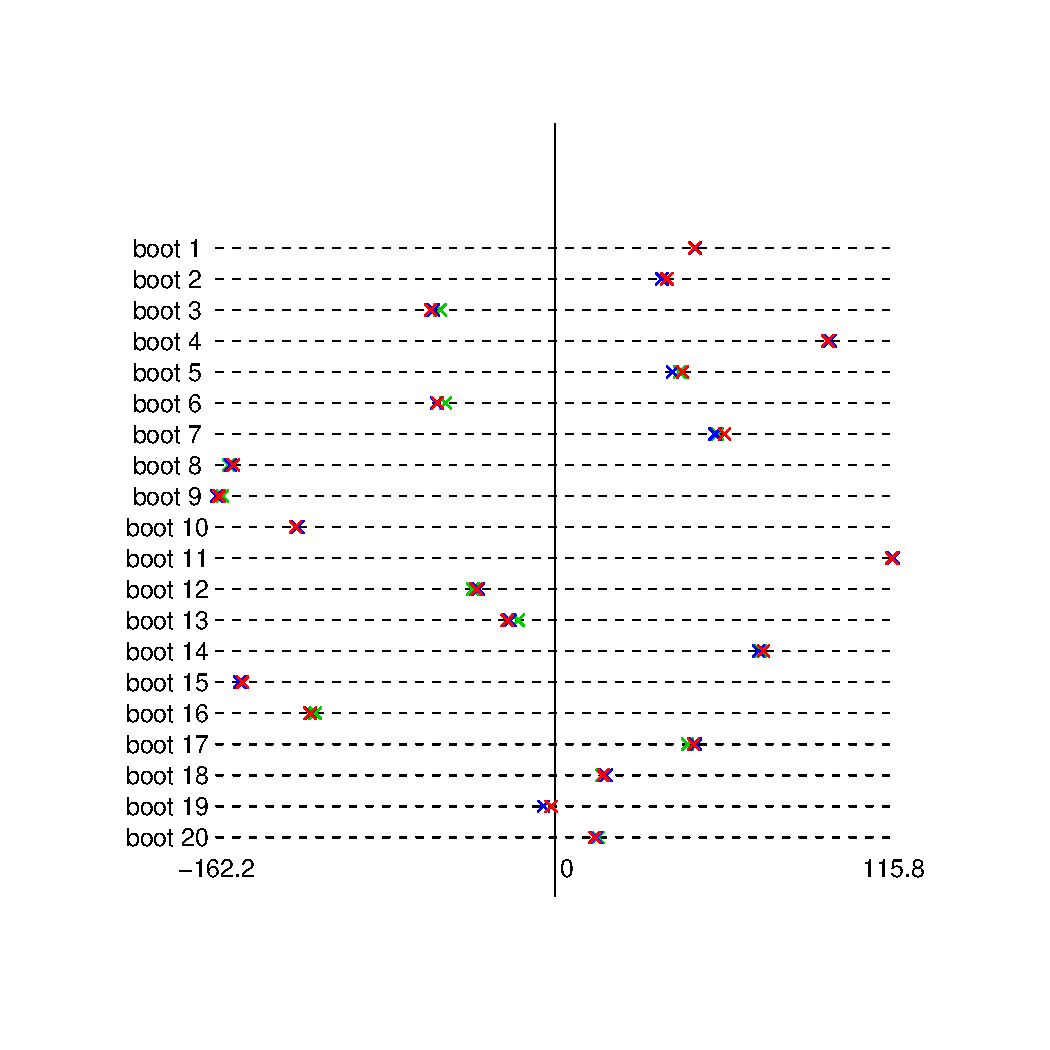
\includegraphics[width=0.48\textwidth]{../newimages/sh_test_centered_plots3.pdf}
    \put(-180,10){\myFigLabel{figCenteredSH3Counter}: SH Test after centering}
   \vspace{-0pt}
   \vspace{-40pt}
  \end{center}
\end{wrapfigure}
\begin{wrapfigure}{r}{0.5\textwidth}
  \begin{center}
   \vspace{-40pt}
    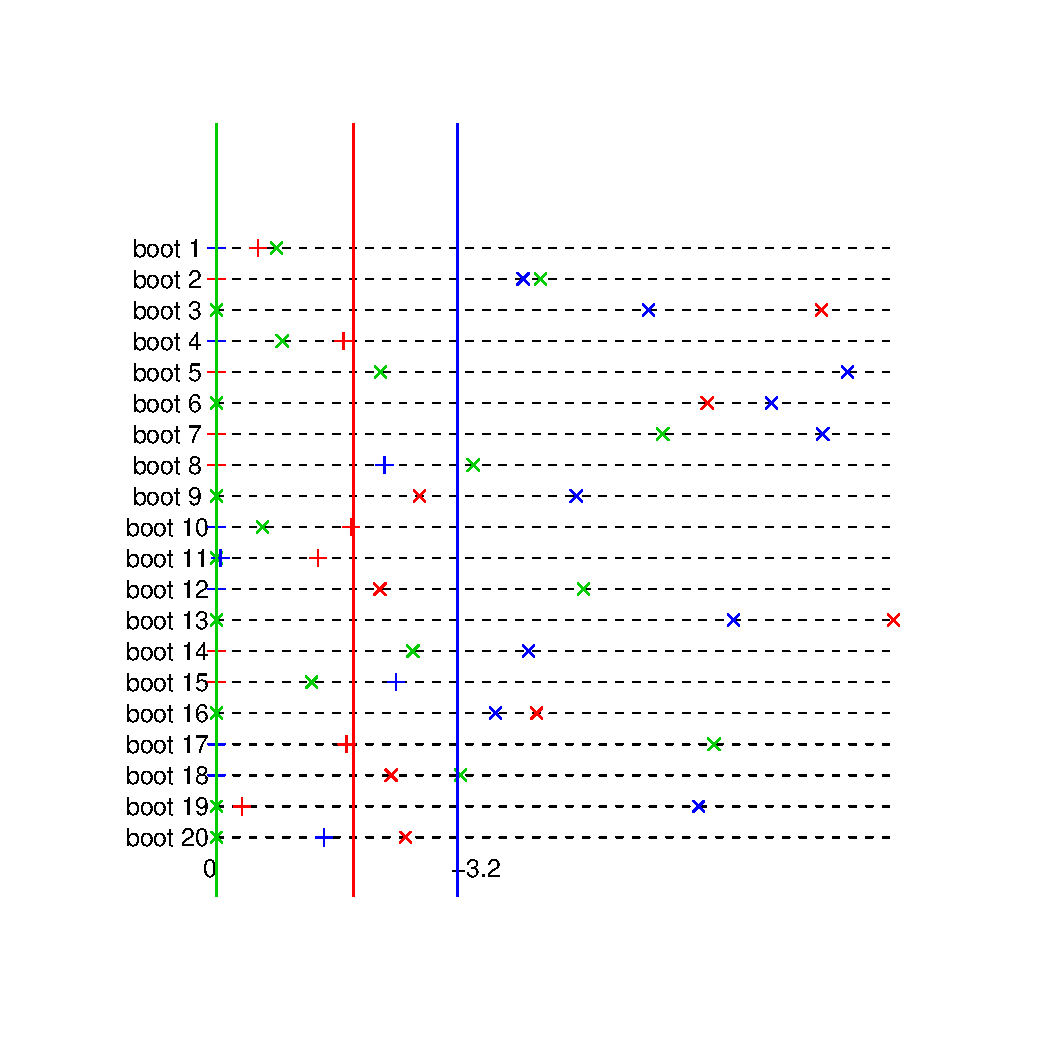
\includegraphics[width=0.48\textwidth]{../newimages/sh_test_stat_plots3.pdf}
    \put(-180,10){\myFigLabel{figSHTestStat3Counter}: SH Test draws from the null }
   \vspace{-0pt}
   \vspace{-20pt}
  \end{center}
\end{wrapfigure}
The SH Test is difficult to represent in figures. 
Figure \arabic{figUncenteredSH3Counter} shows the $\lnL$ values obtained 
for {\color{blue} $T_1$},  {\color{green} $T_2$}, and  {\color{red} $T_3$} from the first 20 replicates of a RELL bootstrap; the vertical lines correspond to the
mean $\lnL$ 
If you look very closely (which would require zooming in on the pdf), you can see that
{\color{green} $T_2$} has the highest $\lnL$ in most of the bootstrap replicates.
This is not surprising, as it is also the tree with the highest $\lnL$ on unperturbed data.

After centering the $\lnL$ values for each tree (Figure \arabic{figCenteredSH3Counter}) by 
subtracting each tree's mean $\lnL$ over all bootstrap reps from each bootstrap value, we obtain a bootstrap estimate of the 
distribution of $\lnL$ values under the null.

Recall that our test statistic on the real data involved comparing the $\lnL$ of the ML tree to the $\lnL$ score for each tree in the candidate set.
The SH Test mimics this by calculating the difference (for each bootstrap replicate) between the maximum centered $\lnL$ and the centered $\lnL$ for each tree.
Each bootstrap replicate in the SH test provides an value of the test statistic for each tree that can be viewed as a draw from the null distribution of the $\delta$ test statistic for  that tree.
By counting the proportion of draws from the null distribution that have a magnitude $\geq$ the magnitude of $\delta(\hat{T},T_i|X)$ we can approximate a \pvalue for each tree $i$ (in the figure the values as extreme as the observed $\delta$ are show with $\times$ symbols, and the draws from the null that are less extreme are shown as $+$).
Note that the ML tree has a $\delta$ statistic of 0. Thus, all of the draws from the null are at least this extreme, and its \pvalue is always 1.0 (and we never reject the ML tree, of course).
The \pvalue for $T_1 \approx 0.3$ and the \pvalue for $T_3 \approx 0.45$ according to the SH Test, so neither tree would be rejected.
\begin{wrapfigure}{r}{0.5\textwidth}
  \begin{center}
   \vspace{-40pt}
    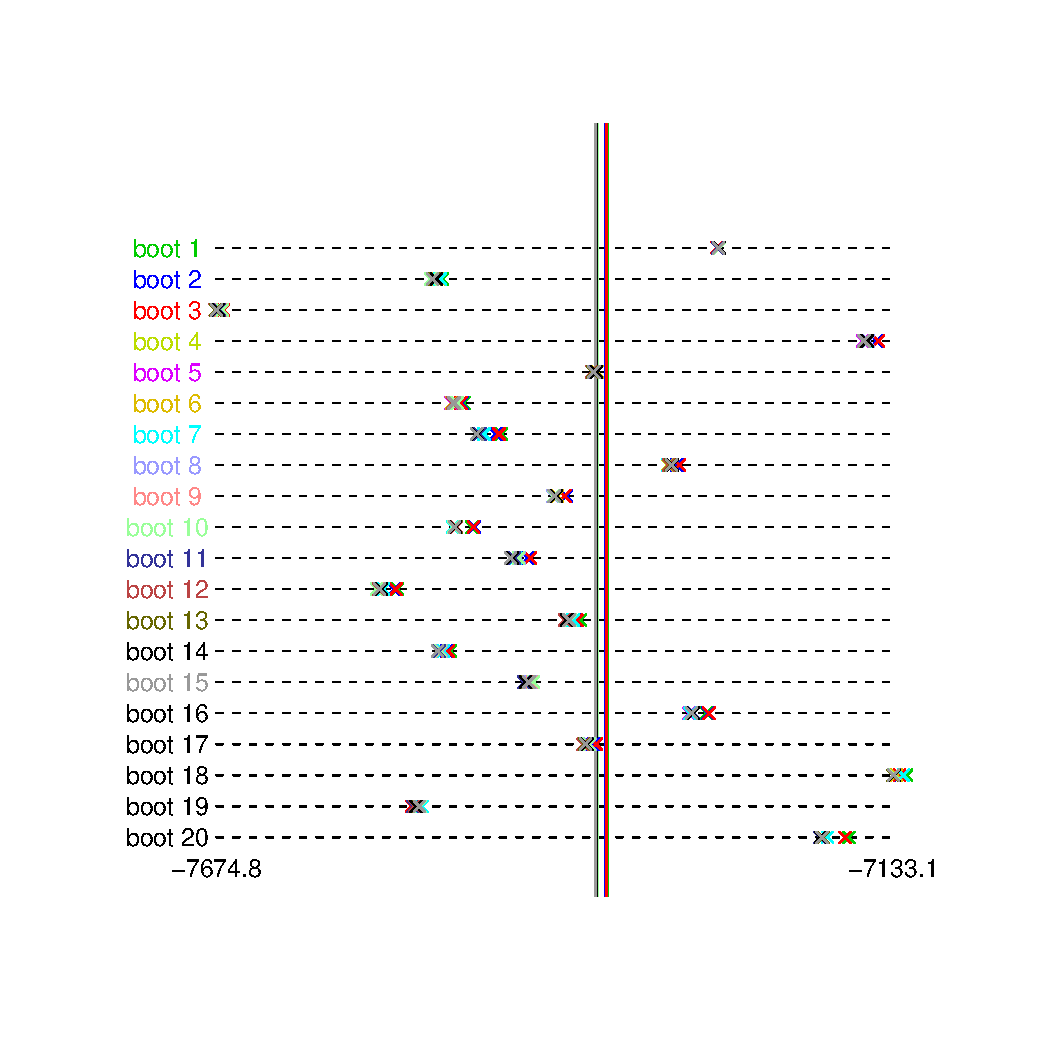
\includegraphics[width=0.48\textwidth]{../newimages/sh_test_uncentered_plots.pdf}
    \put(-200,10){\myFigLabel{figUncenteredSHAllCounter}: SH Test uncentered $\lnL$ }
    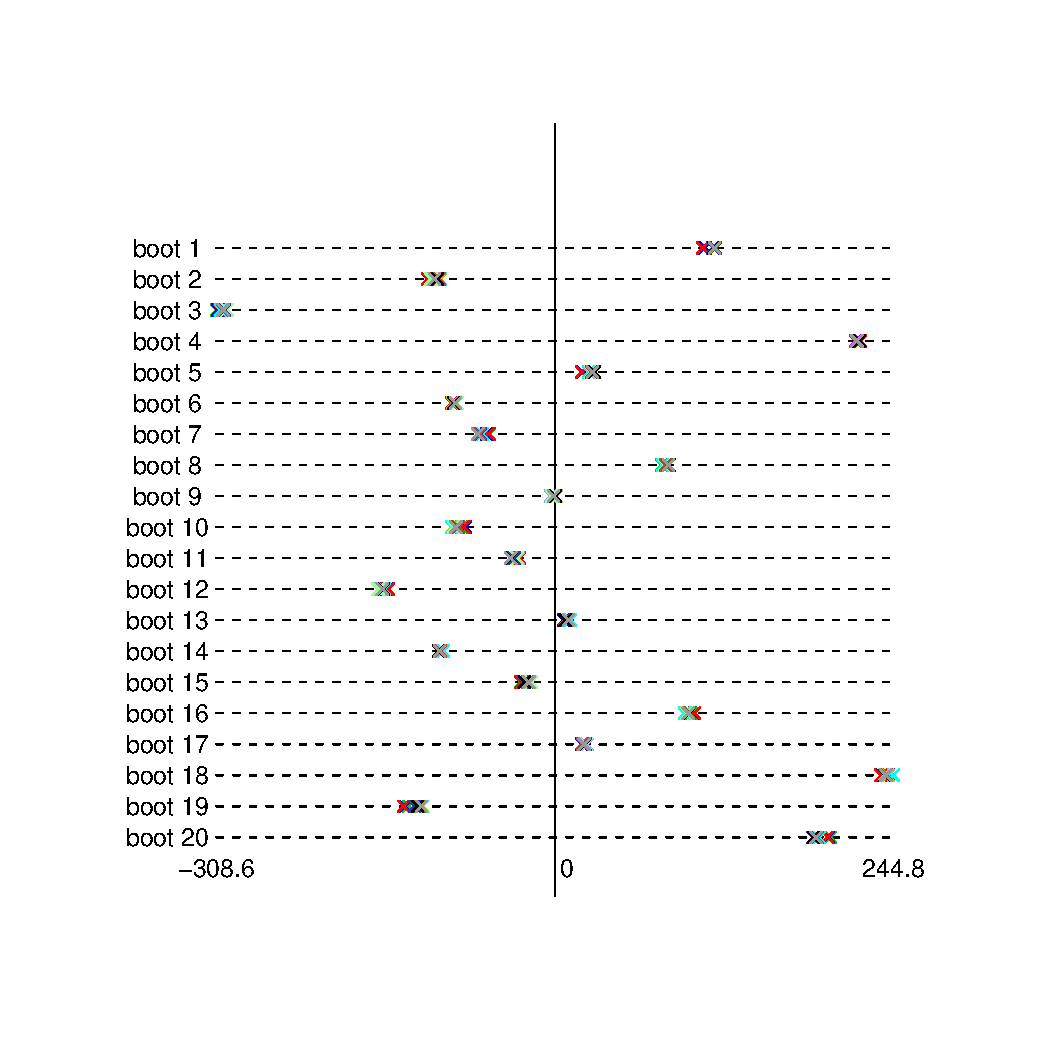
\includegraphics[width=0.48\textwidth]{../newimages/sh_test_centered_plots.pdf}
    \put(-180,10){\myFigLabel{figCenteredSHAllCounter}: SH Test after centering}
   \vspace{-0pt}
   \vspace{-40pt}
  \end{center}
\end{wrapfigure}
\begin{wrapfigure}{r}{0.5\textwidth}
  \begin{center}
   \vspace{-40pt}
    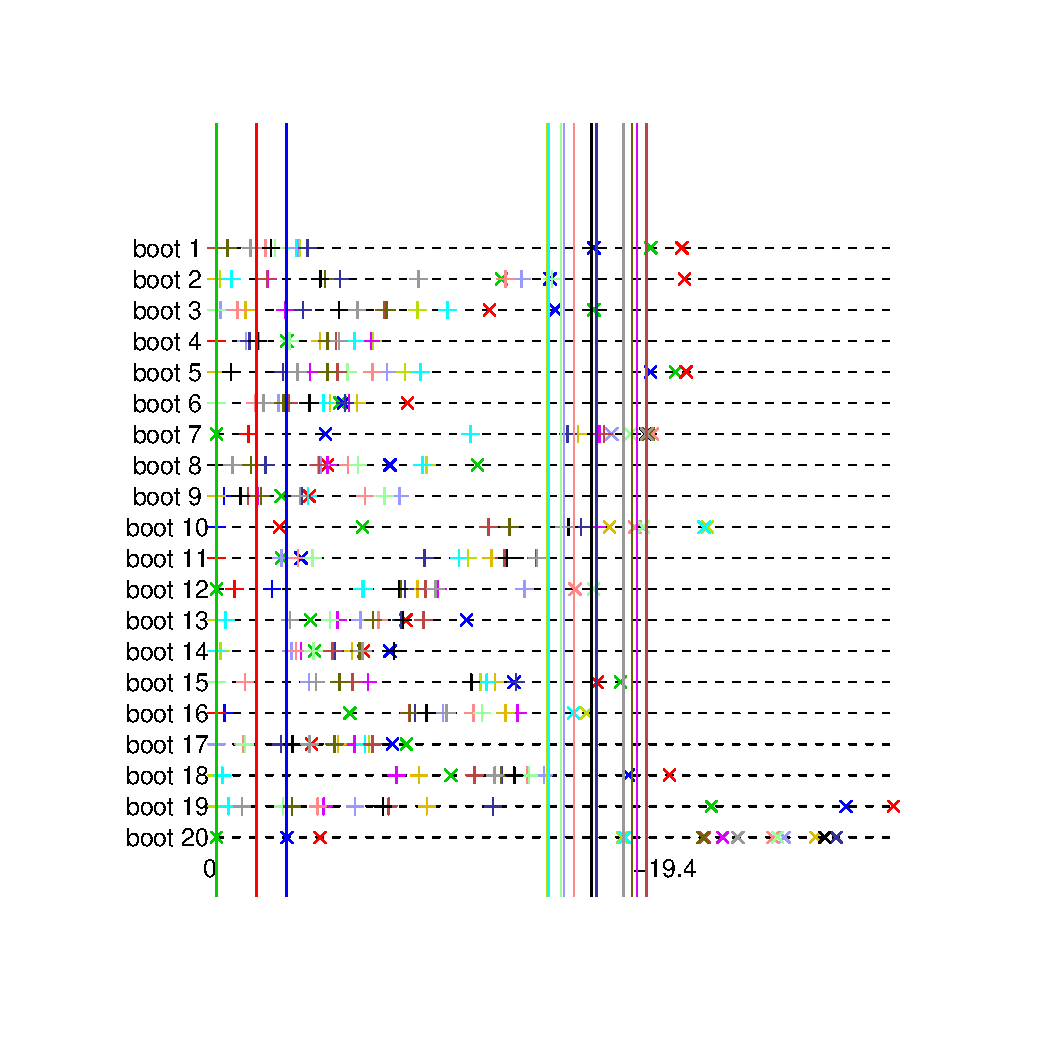
\includegraphics[width=0.48\textwidth]{../newimages/sh_test_stat_plots.pdf}
    \put(-180,10){\myFigLabel{figSHTestStatAllCounter}: SH Test draws from the null }
   \vspace{-0pt}
   \vspace{-20pt}
  \end{center}
\end{wrapfigure}
If our candidate set includes all 15 possible trees (rather than just the trees that have human, chimp, and gorilla as a clade), then we find the SH Test has lower power.
The approximated \pvalues for $T_1$ and $T_3$ are then $0.69$ and  $0.78$ respectively.
Figures \arabic{figUncenteredSHAllCounter} - \arabic{figSHTestStatAllCounter} show the SH procedure on the first twenty bootstrap replicates for all 15 trees.
Even though the other 12 trees that are now in are candidate set do not have high likelihoods (compared to $T_1, T_2$, and $T_3$), including more trees in the candidate set weakens the test.

The SH Test's centering of all of the bootstrapped $\lnL$ values around the same quantity (0) is conservative.
After centering, even a tree with poor fit to the data can achieve the highest centered $\lnL$ score on a bootstrap replicate.
Thus, adding more trees increases the values of the $\delta$ statistic that you would expect under the null. 
This makes the test weaker (because the observed value has to be very extreme to fall in the tails of the broader null distribution).



\newpage
\bibliography{../review/topotesting}

\end{document}

\myNewSlide
\begin{picture}(500,0)(0,0)
	  \put(0,-190){\makebox(0,0)[l]{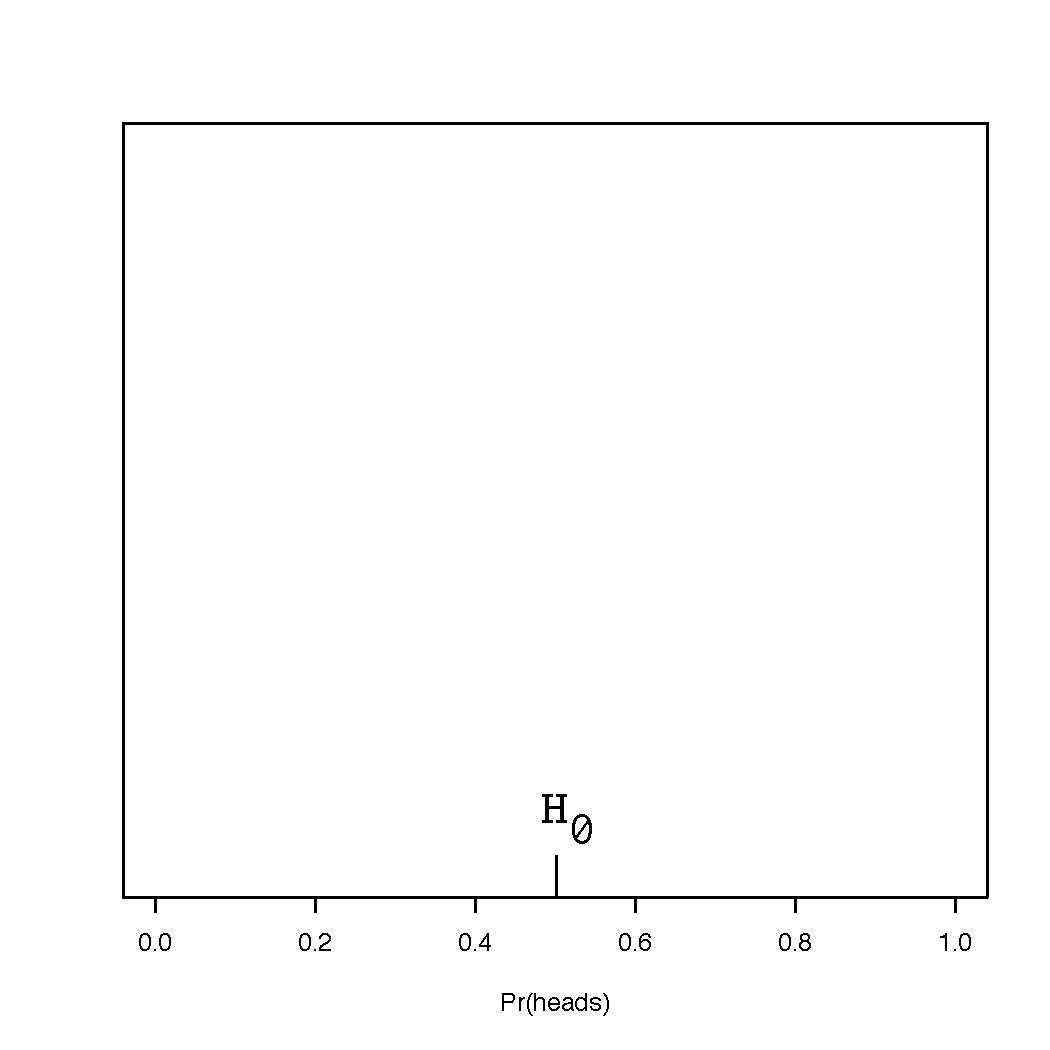
\includegraphics[scale=1.0]{../newimages/coin_axes.pdf}}}
\end{picture}

\myNewSlide
\begin{picture}(500,0)(0,0)
	  \put(0,-190){\makebox(0,0)[l]{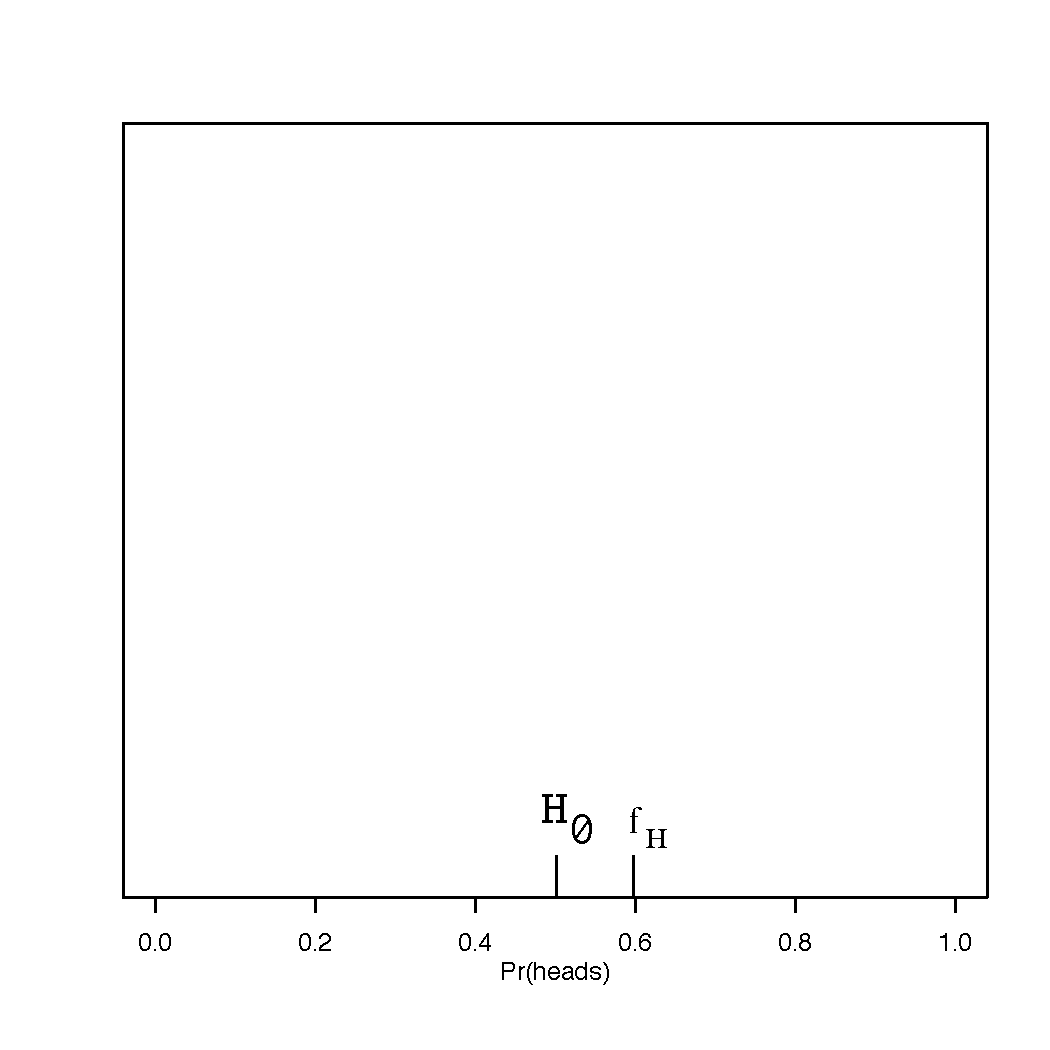
\includegraphics[scale=1.0]{../newimages/coin_axes_data.pdf}}}
\end{picture}

\myNewSlide
\begin{picture}(500,0)(0,0)
	  \put(0,-190){\makebox(0,0)[l]{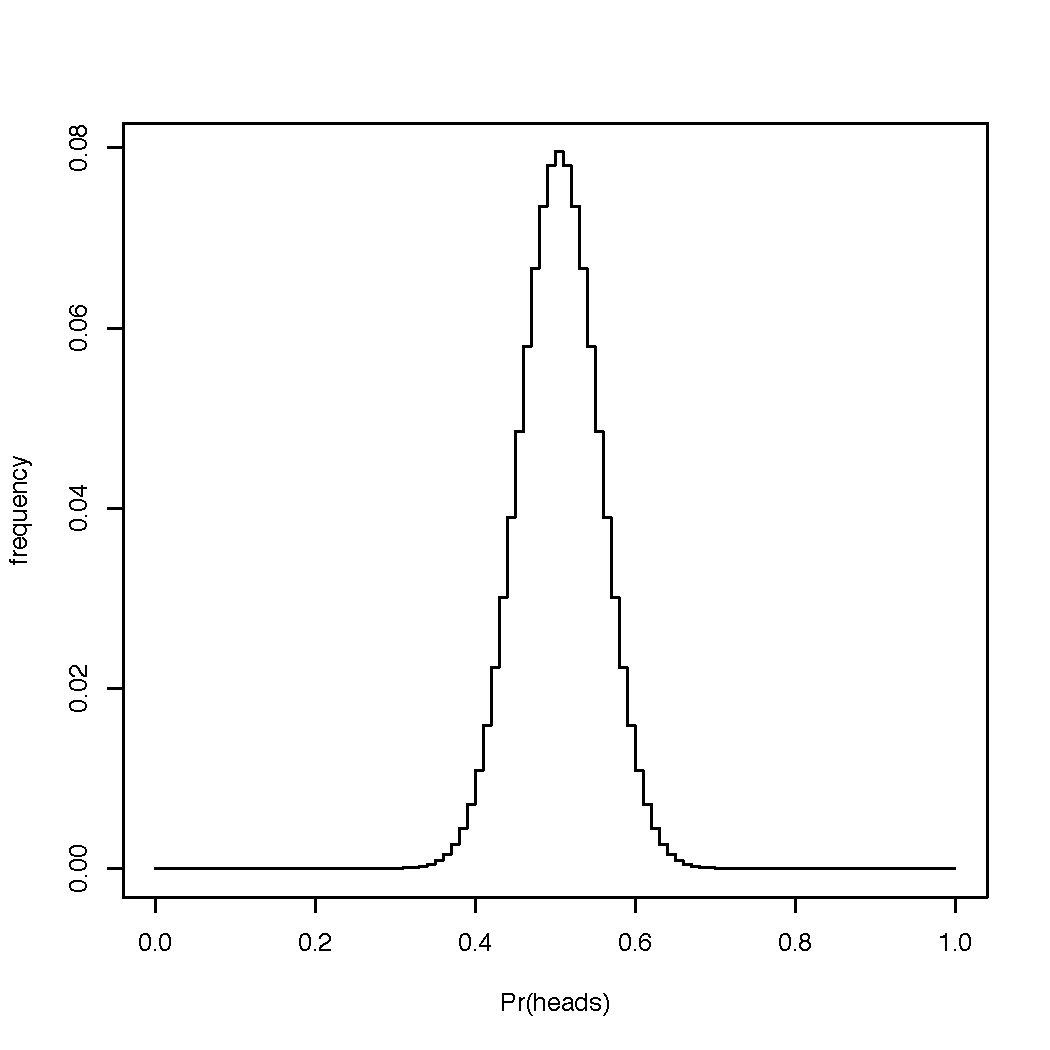
\includegraphics[scale=1.0]{../newimages/coin_wo_tails.pdf}}}
\end{picture}

\myNewSlide
\begin{picture}(500,0)(0,0)
	  \put(0,-190){\makebox(0,0)[l]{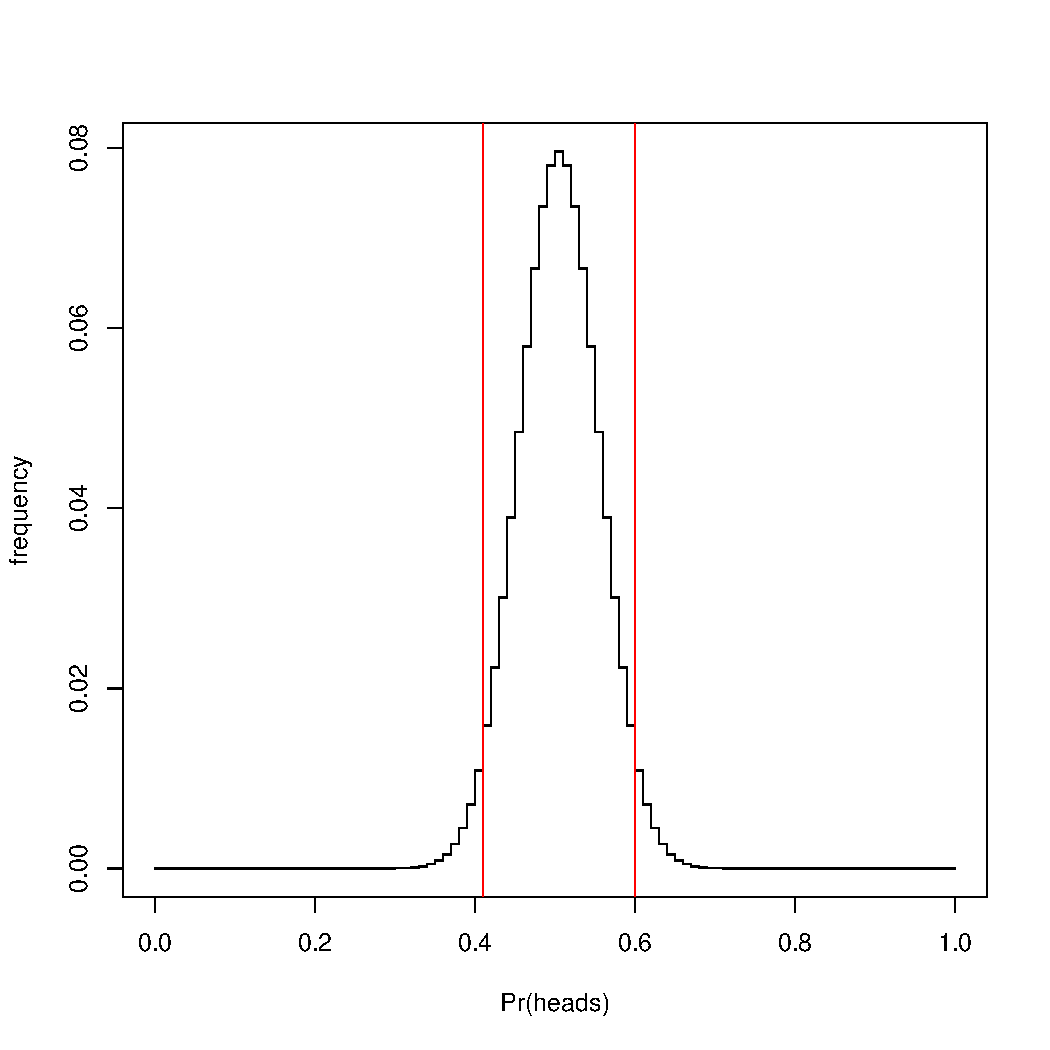
\includegraphics[scale=1.0]{../newimages/coin_w_tails.pdf}}}
	  \put(0,-450){$P$-value $\approx$ 0.058}
\end{picture}

\myNewSlide
Making similar plots for tree inference is hard.

Our parameter space is trees and branch lengths. Our data is a matrix of characters. It is hard to put these objects on the same plot.

We will see later (during ``cartoon time''), that we {\em can} visualize them both in a parameter space that describes how frequent different patterns of data are.


\myNewSlide
\section*{The simplest phylogenetic test would compare two trees}
\Large
Null: If we had no sampling error (infinite data) $T_1$ and $T_2$ would explain the data equally well. 

Test Statistic: 

Expectation under null: $$\mathbb{E}_{H_0}\left[\delta(T_1,T_2|X)\right] = 0$$


\myNewSlide
\begin{picture}(500,0)(-20,-50)
	  \put(20,-20){\small Using 3000 sites of mtDNA sequence for 5 primates}
	  \put(20,-60){\normalsize $T_1$ is ((chimp, gorilla), human)}
	  \put(50,-200){\makebox(0,-190)[l]{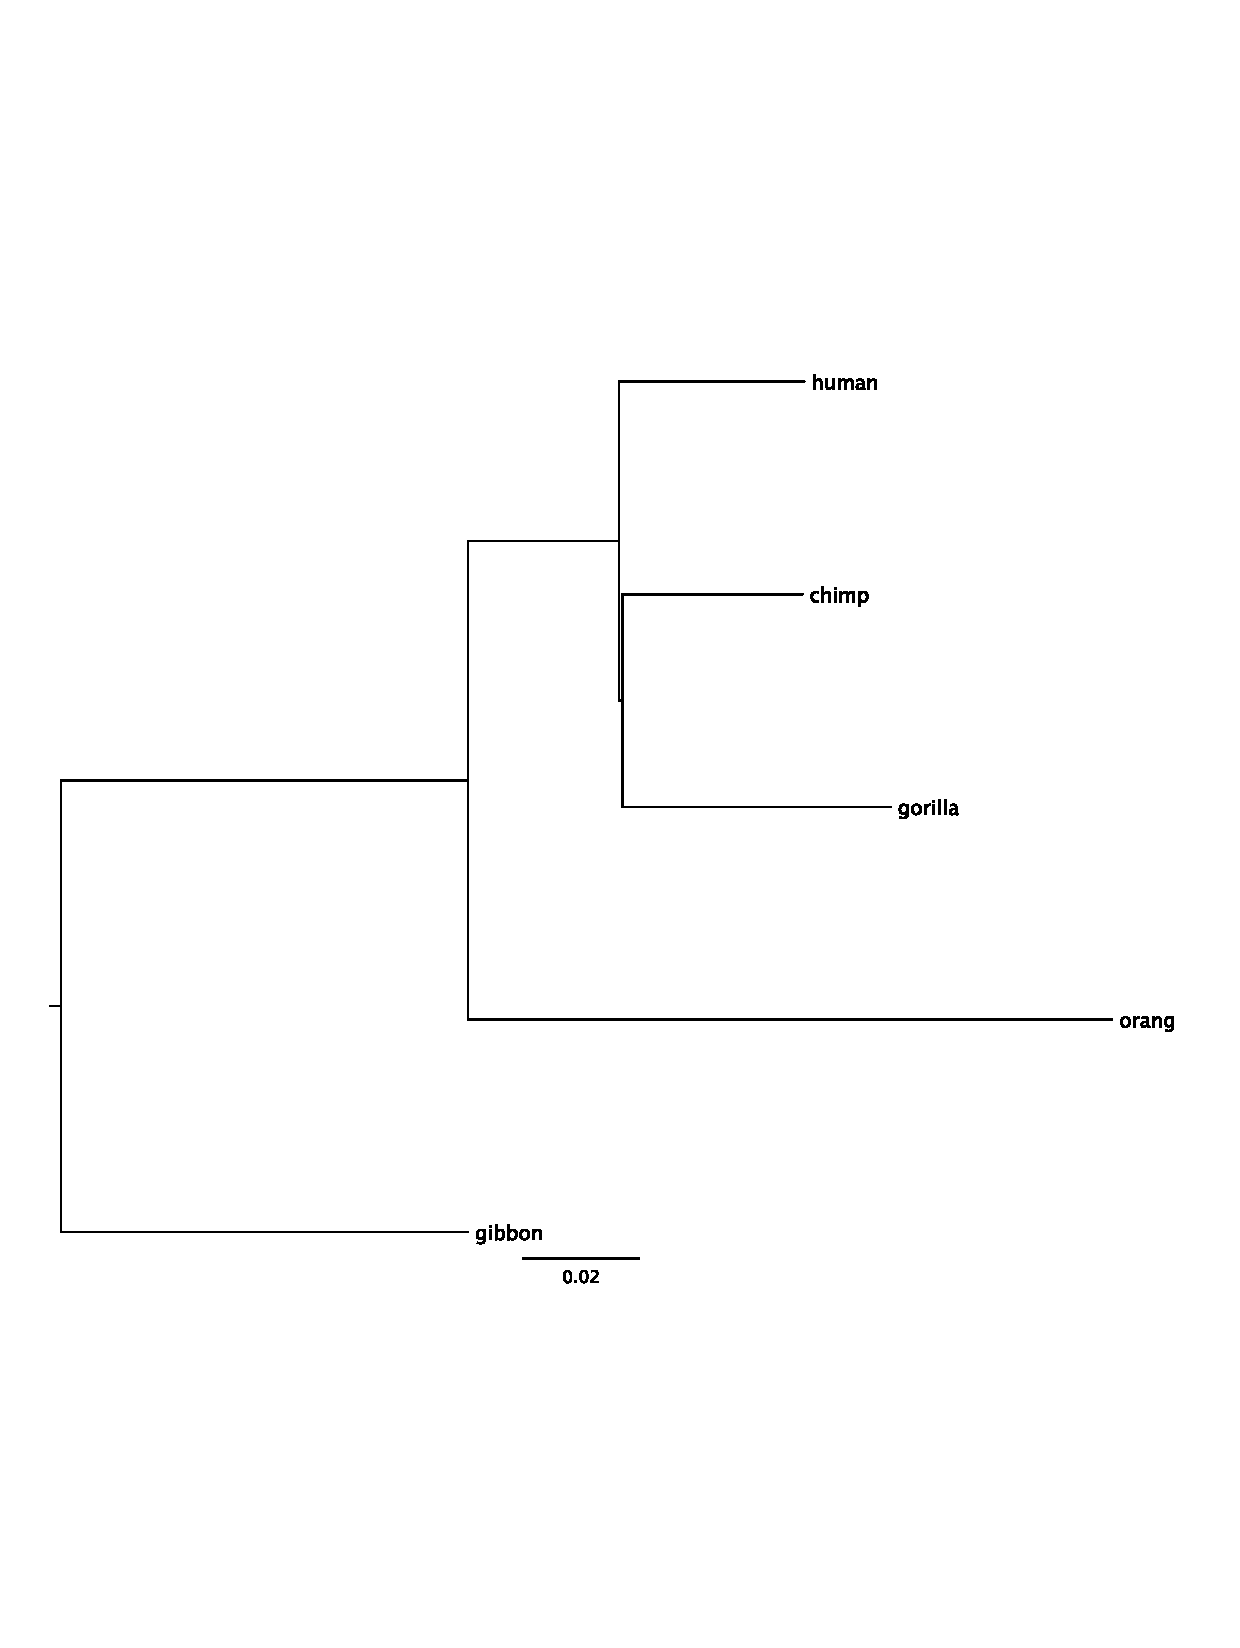
\includegraphics[scale=1.0]{../scripts/mtdna/chimpGorilla3000sites.pdf}}}
\end{picture}

\myNewSlide
\begin{picture}(500,0)(-20,-50)
	  \put(20,-20){\small Using 3000 sites of mtDNA sequence for 5 primates}
	  \put(20,-60){\normalsize $T_2$ is ((chimp, human), gorilla)}
	  \put(50,-200){\makebox(0,-190)[l]{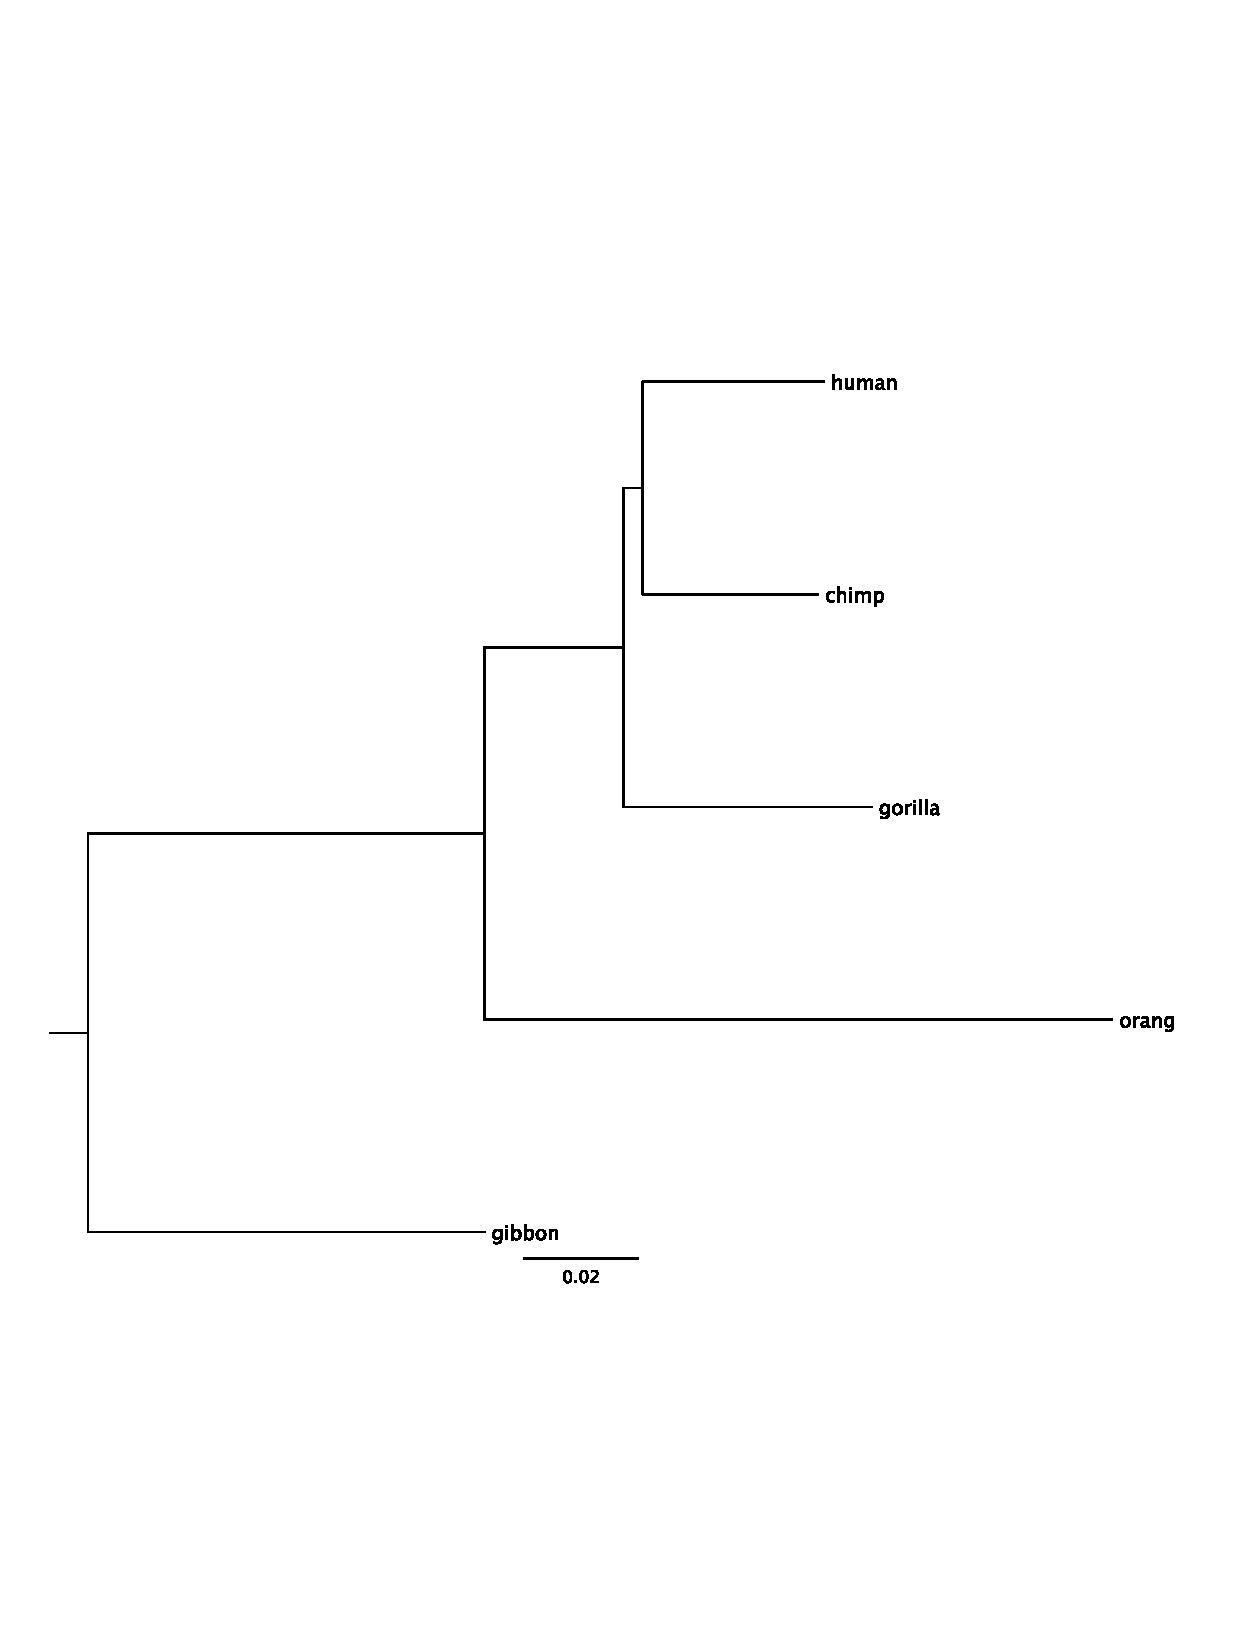
\includegraphics[scale=1.0]{../scripts/mtdna/humanChimp3000SitesTree.pdf}}}
\end{picture}

\myNewSlide
\begin{picture}(500,0)(-20,-50)
	  \put(20,-20){\small Using 3000 sites of mtDNA sequence for 5 primates}
	  \put(20,-60){\normalsize $T_1$ is ((chimp, gorilla), human)   \hskip2cm $\ln L(T_1|X) = -7363.296$}
	  \put(20,-100){\normalsize $T_2$ is ((chimp, human), gorilla)  \hskip2cm $\ln L(T_2|X) = -7361.707$}
	  \put(-10,-385){\small$\delta(T_1,T_2|X)=-3.18$}
	  \put(300,-385){\small$\mathbb{E}(\delta)$}
	  \put(50,-150){\makebox(0,-190)[l]{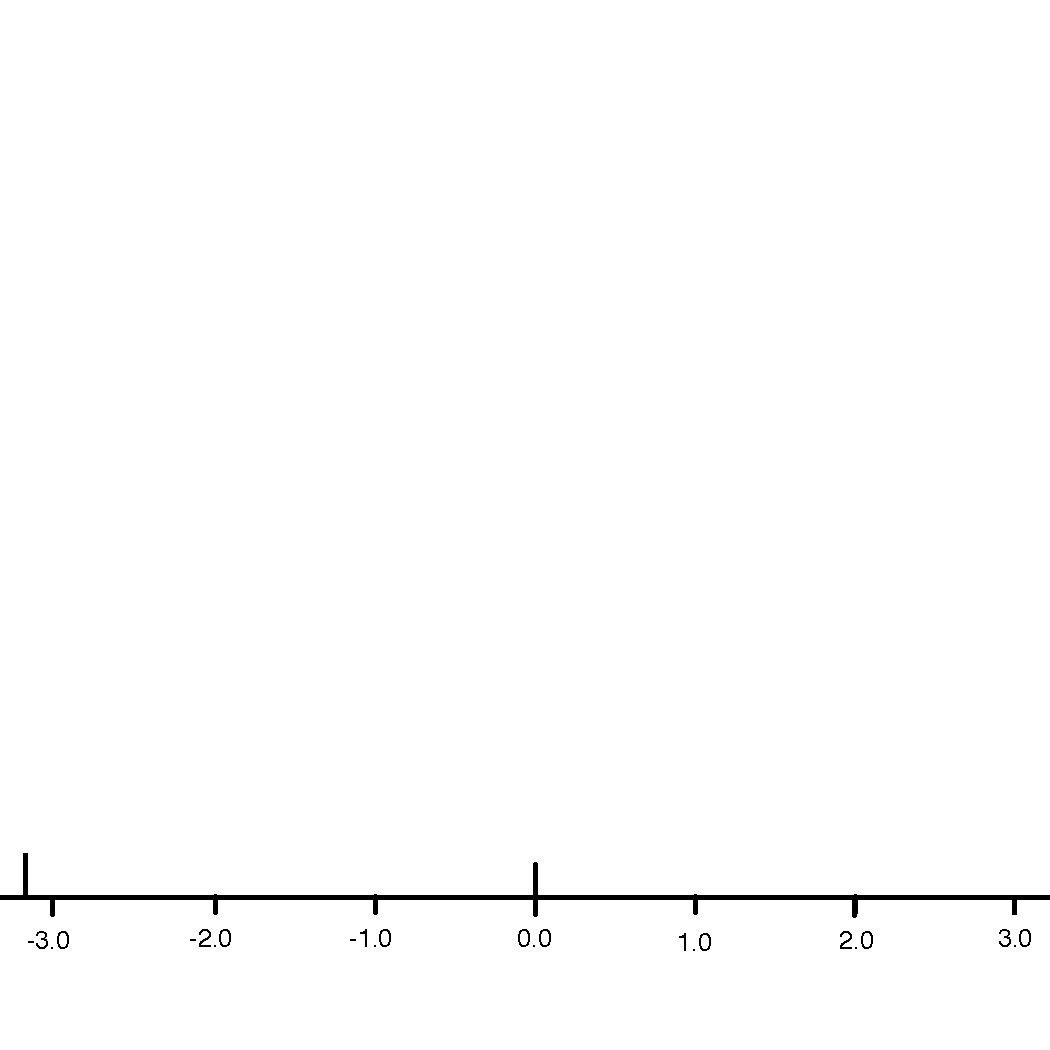
\includegraphics[scale=1.0]{../newimages/delta_axes.pdf}}}
	  \put(220,-480){$\delta(T_1,T_2|X) $}
\end{picture}




\myNewSlide

To get the $P$-value, we need to know the probability: $$\Pr\left(\big|\delta(T_1,T_2|X)\big| \geq 3.18 | H_0\mbox{ is true}\right) $$
\begin{picture}(500,0)(-20,-50)
	  \put(-10,-235){\small$\delta(T_1,T_2|X)=-3.18$}
	  \put(460,-235){\small$-\delta(T_1,T_2|X)=3.18$}
	  \put(10,-270){\huge$\leftarrow$}
	  \put(570,-270){\huge$\rightarrow$}
	  \put(300,-235){\small$\mathbb{E}(\delta)$}
	  \put(50,-0){\makebox(0,-190)[l]{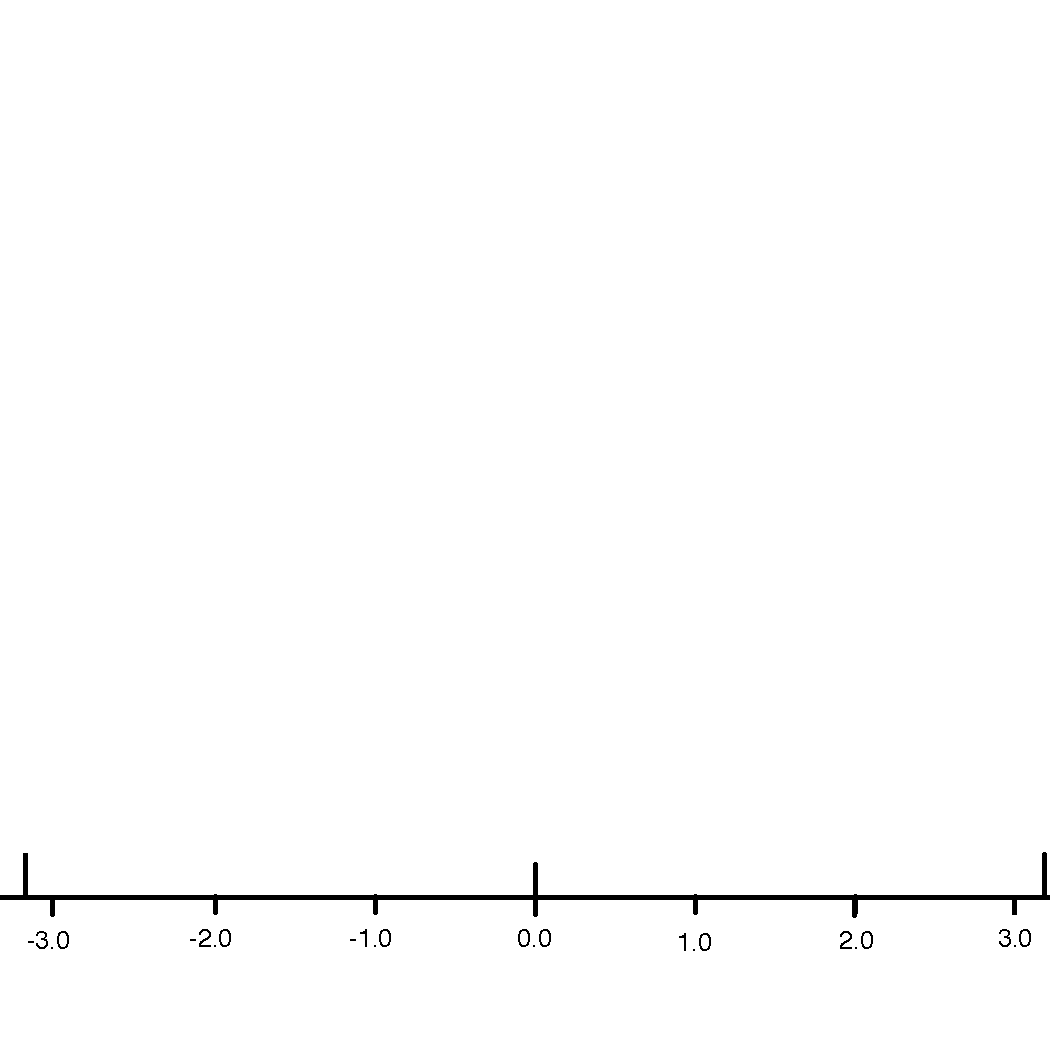
\includegraphics[scale=1.0]{../newimages/delta_axes_reflected.pdf}}}
	  \put(220,-330){$\delta(T_1,T_2|X) $}
\end{picture}

\myNewSlide
\section*{KH Test}
\begin{compactenum}
	\item Examine at the difference in $\ln L$ for each site: $\delta(T_1,T_2|X_i)$ for site $i$.
	\item Note that the total difference is simply a sum:
		$$\delta(T_1,T_2|X) = \sum_{i=1}^M\delta(T_1,T_2|X_i)$$
	\item The variance of $\delta(T_1,T_2|X)$ will be a function of the variance in ``site'' $\delta(T_1,T_2|X_i)$ values.
\end{compactenum}



\myNewSlide
\begin{picture}(500,0)(0,0)
	  \put(0,10){\large $\delta(T_1,T_2|X_i)$ for each site, $i$.}
	  \put(280,-35){\large $\vdots$}
	  \put(20,-250){\makebox(0,0)[l]{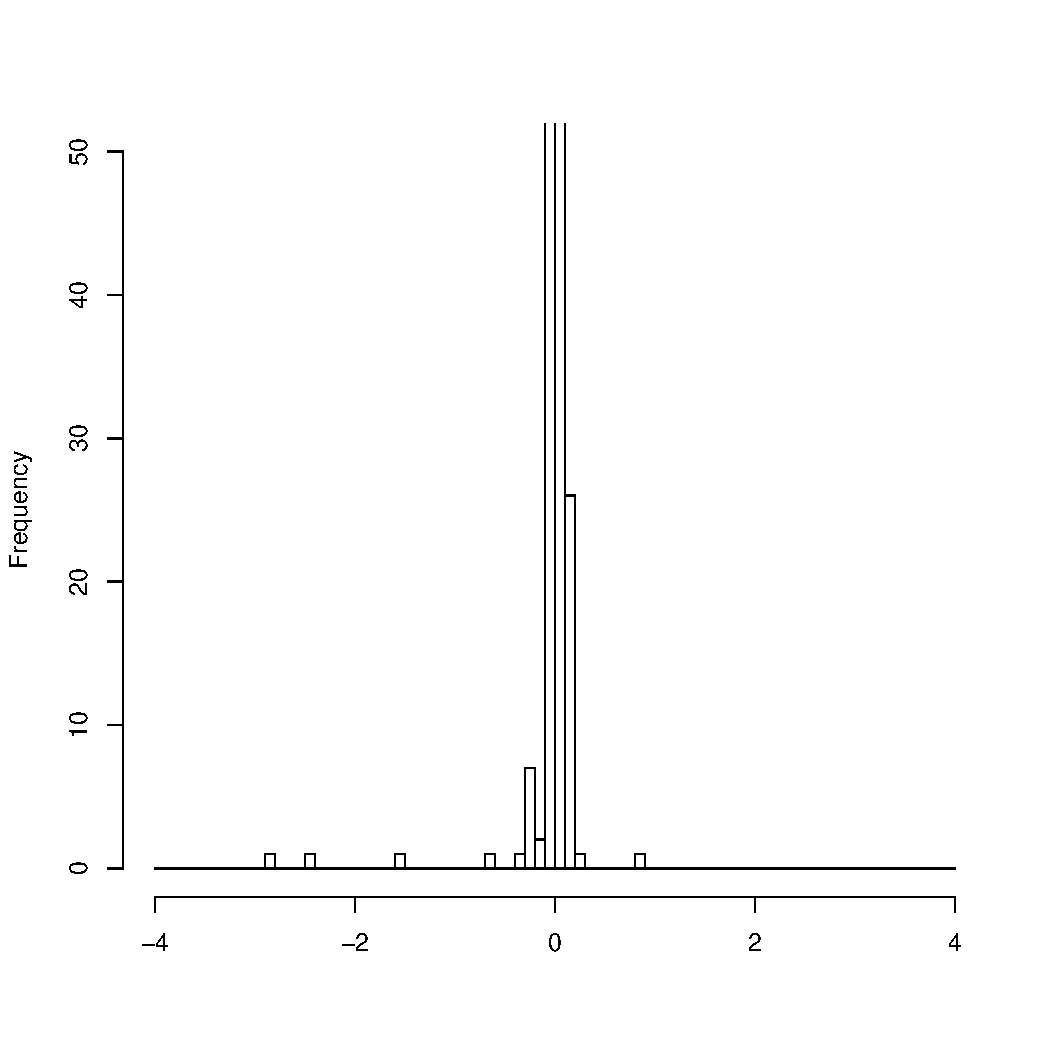
\includegraphics[scale=1.0]{../scripts/mtdna/d1-2hist.pdf}}}
	  \put(250,-490){\normalsize$\delta(T_1,T_2|x_i)$}
\end{picture}


\myNewSlide
\section*{KH Test - the variance of $\delta(T_1,T_2|X)$}
To get a sense of the variance of $\delta(T_1,T_2|X)$ we should expect because of sampling error, we could use:
\begin{compactenum}
	\item Assumptions of Normality (by appealing to the Central Limit Theorem), or
	\item Bootstrapping to generate a cloud of pseudo-replicate $\delta(T_1,T_2|X^{\ast})$ values.
\end{compactenum}

\myNewSlide
\section*{RELL bootstrap}
\large
If the MLE of the numerical parameters (including branch lengths) do not change much when we bootstrap we can simply resample the site $\ln L$ values and sum them.

This is called the RELL bootstrap \citep[][and Felsenstein]{KishinoMH1990}. It is not a ``safe'' replacement for normal bootstrapping \citep[especially on large trees;][]{StamatakisHR2008} when you want to estimate clade support.

But it should be good enough for helping us learn about the standard error of the $\ln L$.

And it is really fast.

\myNewSlide
\begin{picture}(500,0)(0,0)
	  \put(0,-10){\large $\delta$ for many (RELL) bootstrapped replicates of the data}
	  \put(20,-250){\makebox(0,0)[l]{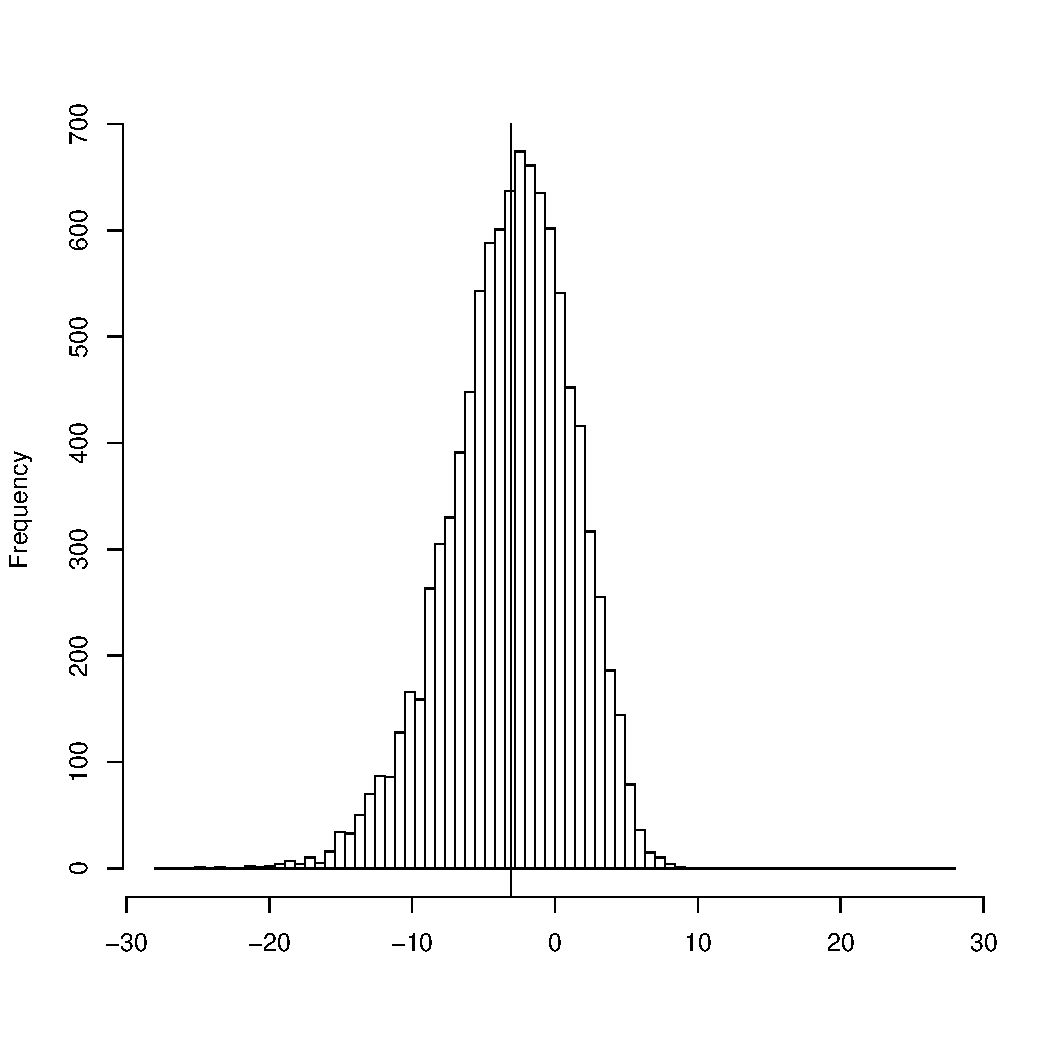
\includegraphics[scale=1.0]{../scripts/mtdna/uncentered1-2hist.pdf}}}
	  \put(250,-490){\normalsize$\delta(T_1,T_2|X^{\ast})$}
\end{picture}

\myNewSlide
\section*{KH Test - `centering'}
$H_0$ gives us the expected value: $$\mathbb{E}_{H_0}\left[\delta(T_1,T_2|X)\right] = 0$$
Bootstrapping gives us a reasonable guess of the variance under $H_0$

By substracting the mean of the bootstrapped $\delta(T_1,T_2|X^{\ast})$ values, we can create a null distribution.

For each of the $j$ bootstrap replicates, we treat $$\delta(T_1,T_2|X^{\ast j}) - \bar\delta(T_1,T_2|X^{\ast})$$  as draws from the null distribution.

\myNewSlide
\begin{picture}(500,0)(0,0)
	  \put(0,10){\large $\delta(T_1,T_2|X^{(j)})-\bar\delta(T_1,T_2|X^{\ast})$}
	  \put(0,-25){for many (RELL) bootstrapped replicates of the data}
	  \put(20,-250){\makebox(0,0)[l]{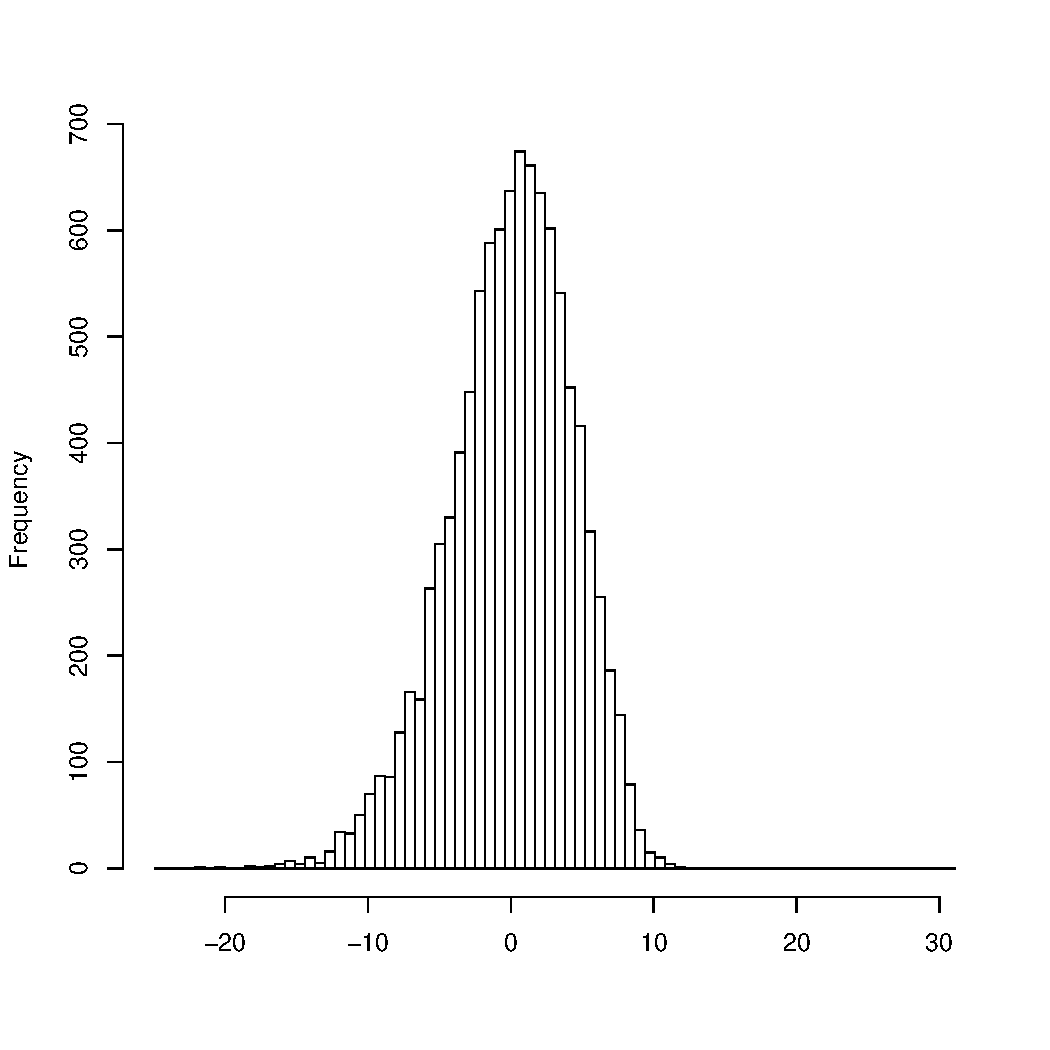
\includegraphics[scale=1.0]{../scripts/mtdna/centered1-2hist.pdf}}}
	  \put(150,-490){\normalsize$\delta(T_1,T_2|X^{(j)})-\bar\delta(T_1,T_2|X^{\ast})$}
\end{picture}

\myNewSlide
\begin{picture}(500,0)(0,0)
	  \put(0,10){\large $\delta(T_1,T_2|X^{(j)})-\bar\delta(T_1,T_2|X^{\ast})$}
	  \put(0,-25){for many (RELL) bootstrapped replicates of the data}
	  \put(20,-250){\makebox(0,0)[l]{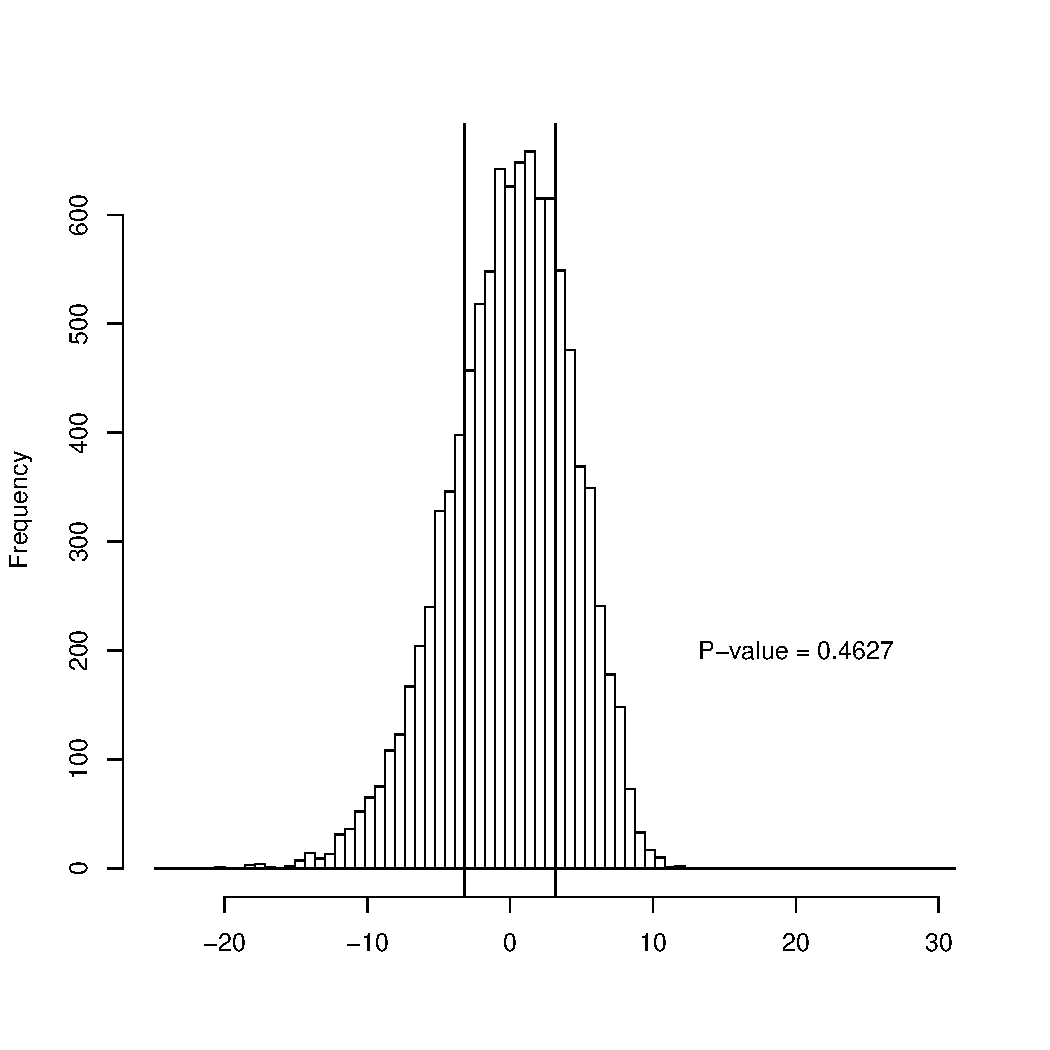
\includegraphics[scale=1.0]{../scripts/mtdna/centered1-2hist-p.pdf}}}
	  \put(250,-490){\normalsize$\delta(T_1,T_2|X^{\ast})-\bar\delta(T_1,T_2|X^{\ast})$}
\end{picture}


\myNewSlide
\section*{What if start out with only one hypothesized tree, and we want to compare it to the ML tree?}
The KH Test is {\bf NOT} appropriate in this context \citep[see][for discussion of this point]{GoldmanAR2000}
	
{\bf Multiple Comparisons}: lots of trees increases the variance of $\delta(\hat{T},T_1|X)$\\

{\bf Selection bias}: Picking the ML tree to serve as one of the hypotheses invalidates the centering procedure of the KH test.

\myNewSlide
\section*{Using the ML tree in your test introduces selection bias}
Even when the $H_0$ is true, we do not expect $2\left[\ln L(\hat{T}) - \ln L(T_1)\right]= 0$

Imagine a competition in which a large number of equally skilled people compete, and you compare the score of one competitor against the highest scorer.

\myNewSlide
\begin{picture}(500,0)(0,0)
	  \put(-10,15){Experiment: 70 people each flip a fair coin 100 times and}
	  \put(0,-20){count \# heads.  Test statistic:}
	  \put(100,-55){$h_1 - h_2$}
	  \put(400,-55){$\max(h) - h_1$}
	  \put(-30,-250){\makebox(0,0)[l]{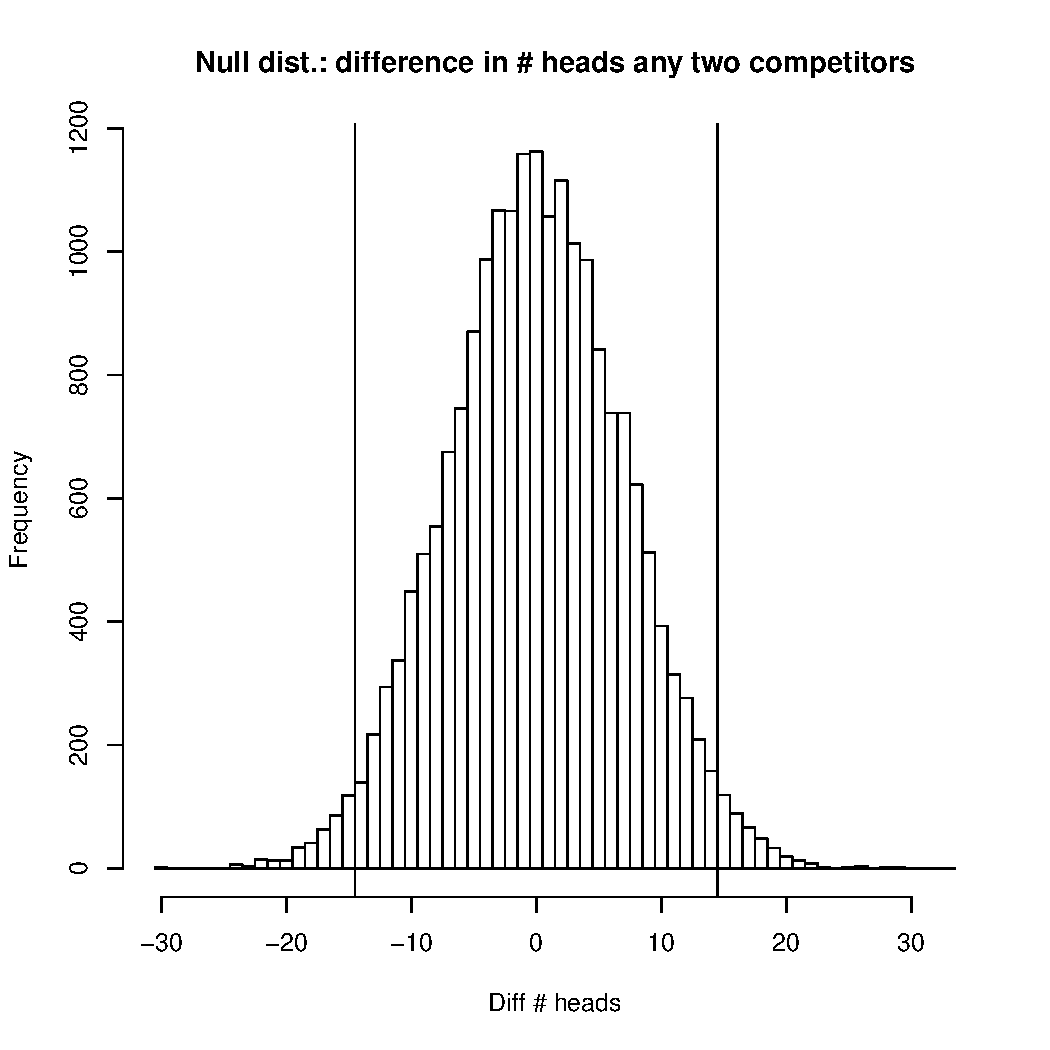
\includegraphics[scale=.75]{../scripts/cfc_diff_a_priori.pdf}}}
	  \put(320,-250){\makebox(0,0)[l]{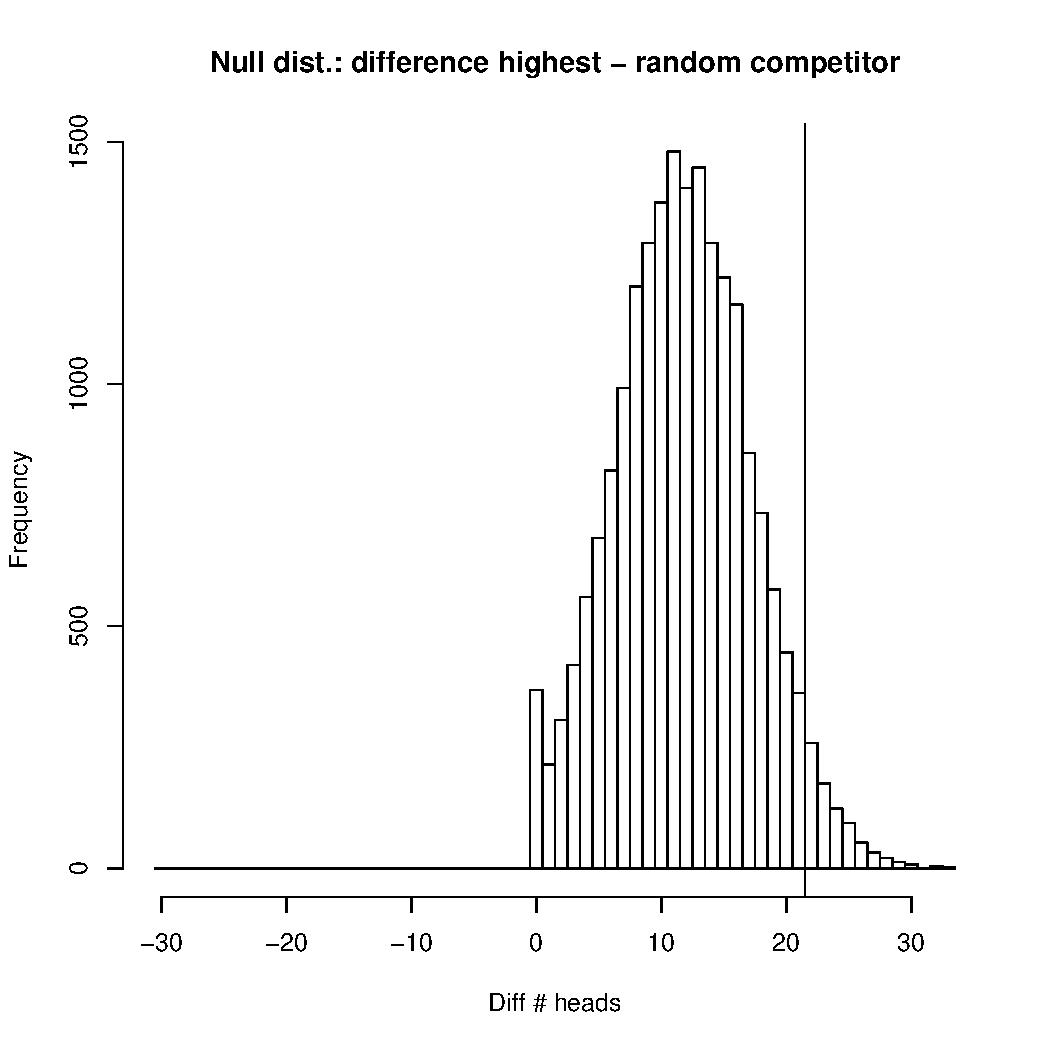
\includegraphics[scale=.75]{../scripts/cfc_diff_best_v_one.pdf}}}
\end{picture}


\myNewSlide 
\section*{Shimodaira and Hasegawa proposed the SH test which deals the ``selection bias'' introduced by using the ML tree in your test}
You have to specify of a set of candidate trees - inclusion in this set {\bf must not} depend on the dataset to be analyzed.

The null hypothesis is that all members of the candidate set have the same expected score.

\myNewSlide
{\bf SH Test details}
\normalsize
\begin{compactitem}
	\item For each tree $T_i$ in the candidate set calculate $\delta(\hat{T}, T_i|X)$
	\item Bootstrap to generate ${\ln L}(T_i|X^{(j)})$
	\item For each tree $T_i$, use $\bar{\ln L}(T_i|X^{\ast})$ to center the bootstrapped collection of log-likelihoods:
		$$c_i^{(j)} = {\ln L}(T_i|X^{(j)})-\bar{\ln L}(T_i|X^{\ast})$$
	\item For each replicate pick the highest value from the centered distributions (this mimics the selection bias): $$m^{(j)} = \max\left[c_i^{(j)}\right] \mbox{ over all } j$$
	\item The for each tree and replicate, you get a sample from the null $\delta_i^{(j)} = m^{(j)} - c_i^{(j)}$
	\item $P$-value for tree $T_i$ can be approximated by seeing where in the distribution of $\delta_i^{(j)}$ values it lies (the $P$-value is the proportion of sampled $\delta_i^{(j)} \geq \delta_i$
\end{compactitem}

\myNewSlide
\section*{SH test candidate set selection}
\large
\begin{compactitem}
	\item The candidate set should be all trees that you would have seriously entertained before seeing the data. 
	\item Using all trees is safe (though weakens the test, and is computationally demanding).
	\item Unfortunately, only considering a subset of trees for computational convenience can invalidate the test.
	\item If a tree has low $\ln L$ and low variance of site-log-likelihoods then it can probably be safely removed without affecting the $P$-values of other trees\footnote{Because such a tree would be unlikely to ever be the tree that is the determines the maximum diplacement from the centered value, $m^{(j)}$.}
\end{compactitem}
The test makes worst-case assumptions, so the SH test {\bf is too conservative}.

\myNewSlide
\large
\begin{picture}(500,0)(0,0)
	  \put(-200,-190){\makebox(0,0)[l]{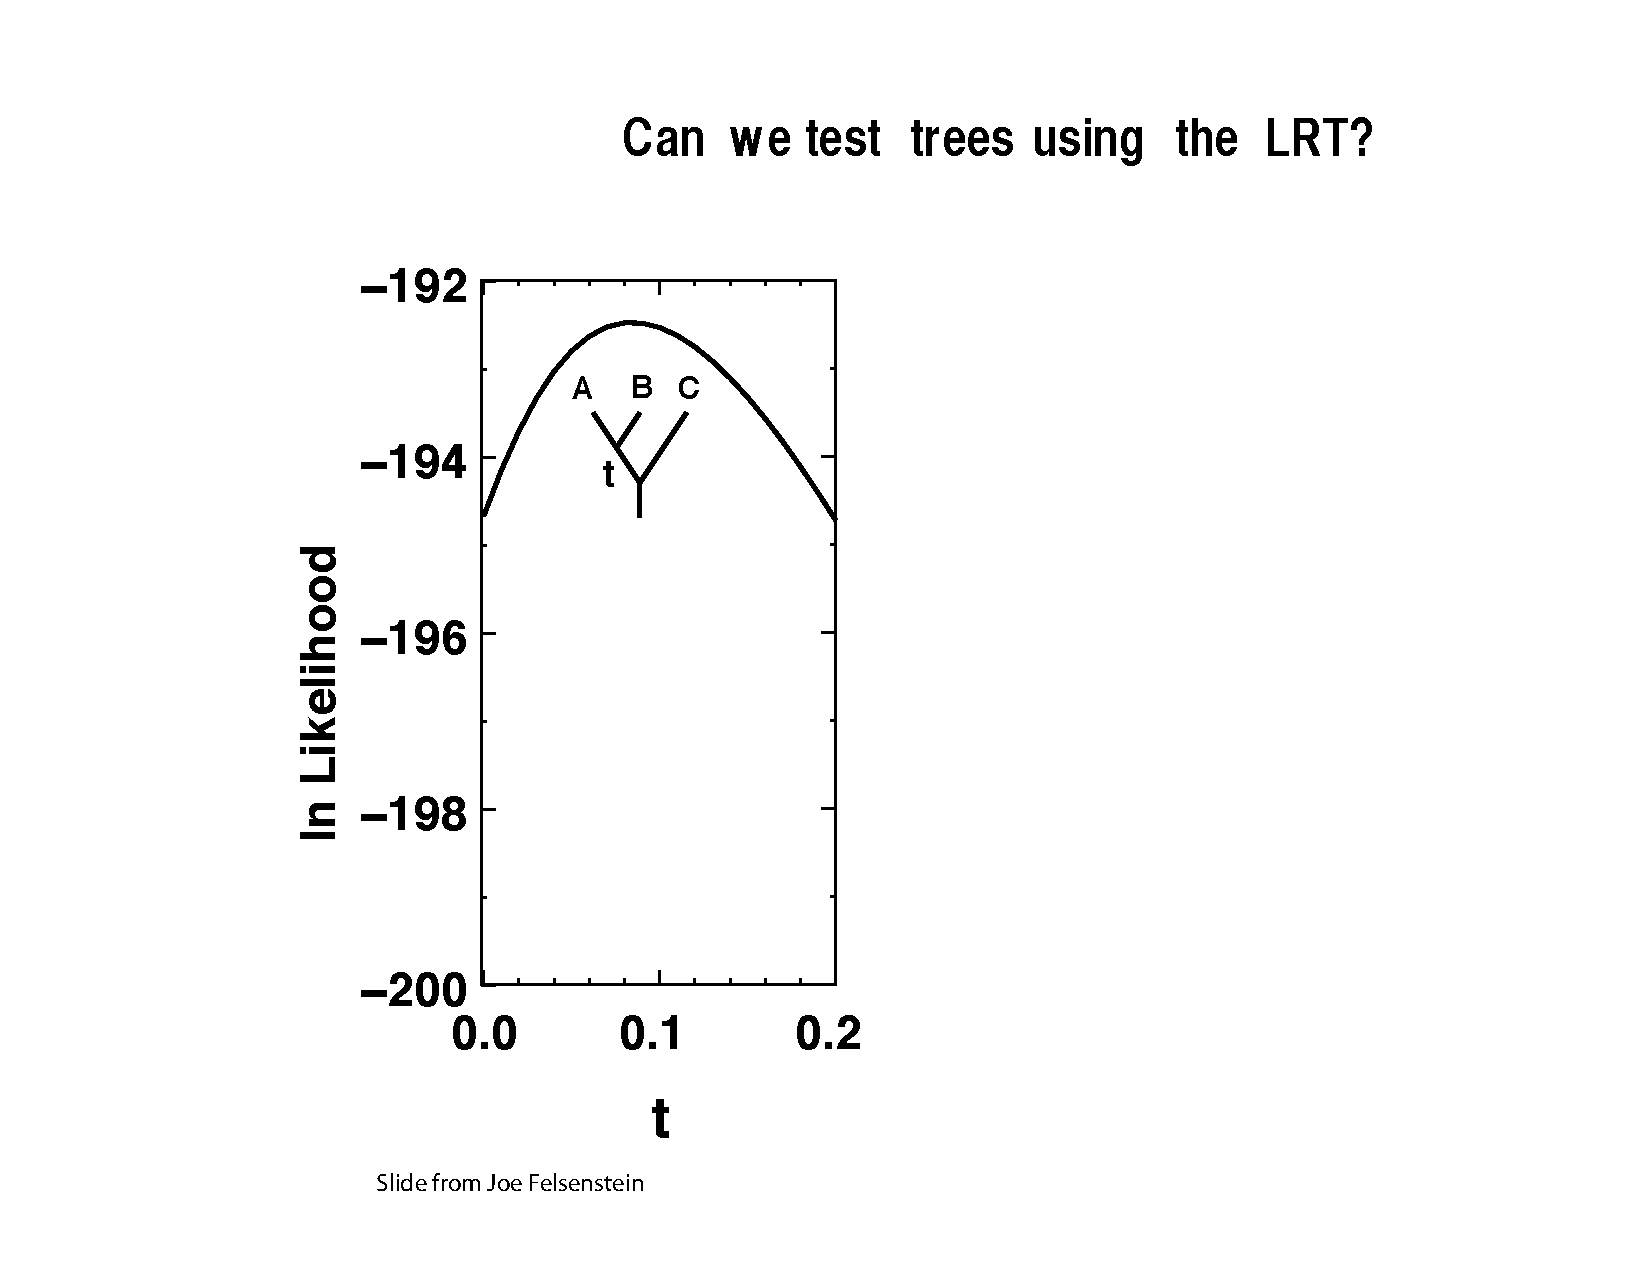
\includegraphics[scale=1.0]{../newimages/JoeFelsTreeLRT1.pdf}}}
	  \put(250,-100){1. Should we calculate the LRT as:}
	  \put(230,-140){$\delta_i = 2\left[\ln L(t=\hat{t},T_i|X) - \ln L(t=0,T_i|X)\right]$}
	  \put(250,-250){2. And can we use the $\chi_1^2$ distribution to}
	  \put(250,-290){get the critical value for $\delta$?}
\end{picture}

\myNewSlide
\begin{picture}(500,0)(0,0)
	  \put(-200,-190){\makebox(0,0)[l]{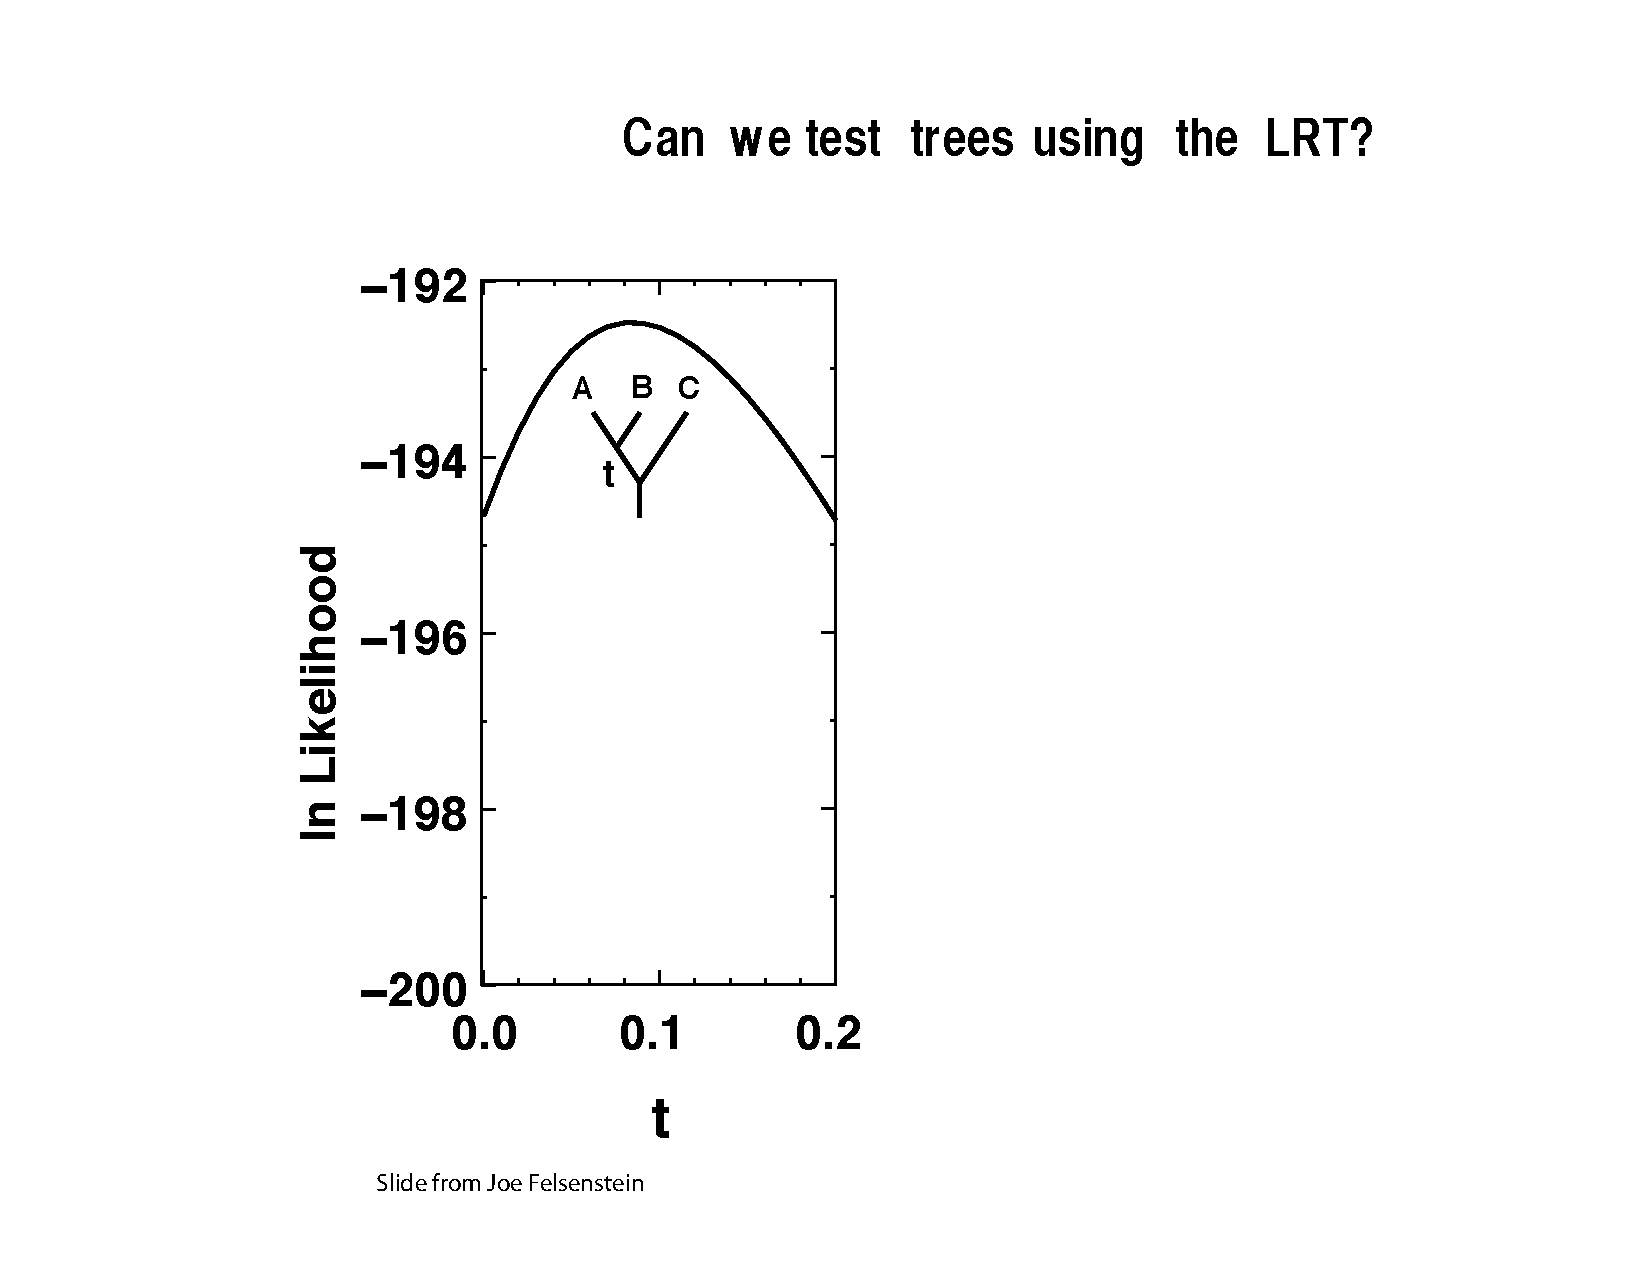
\includegraphics[scale=1.0]{../newimages/JoeFelsTreeLRT1.pdf}}}
	  \put(250,-100){1. Should we calculate the LRT as:}
	  \put(230,-140){$\delta_i = 2\left[\ln L(t=\hat{t},T_i|X) - \ln L(t=0,T_i|X)\right]$}
	  \put(250,-180){{\bf \color{red}No. $t=0$ might not yield the best}}
	  \put(260,-220){\bf\color{red} alternative $\ln L$}
	  \put(250,-290){2. And can we use the $\chi_1^2$ distribution to}
	  \put(250,-330){get the critical value for $\delta$ ?}
	  \put(250,-370){{\bf \color{red}No. Constraining parameters}}
	  \put(260,-410){{\bf \color{red}at boundaries leads to a mixture}}
	  \put(260,-450){{\bf \color{red}such as: $\frac{1}{2}\chi_0^2 + \frac{1}{2}\chi_1^2$}}
	  \put(260,-490){\small See \citet{OtaWHSK2000}.}
\end{picture}

\myNewSlide
\begin{picture}(500,0)(0,0)
	  \put(-200,-190){\makebox(0,0)[l]{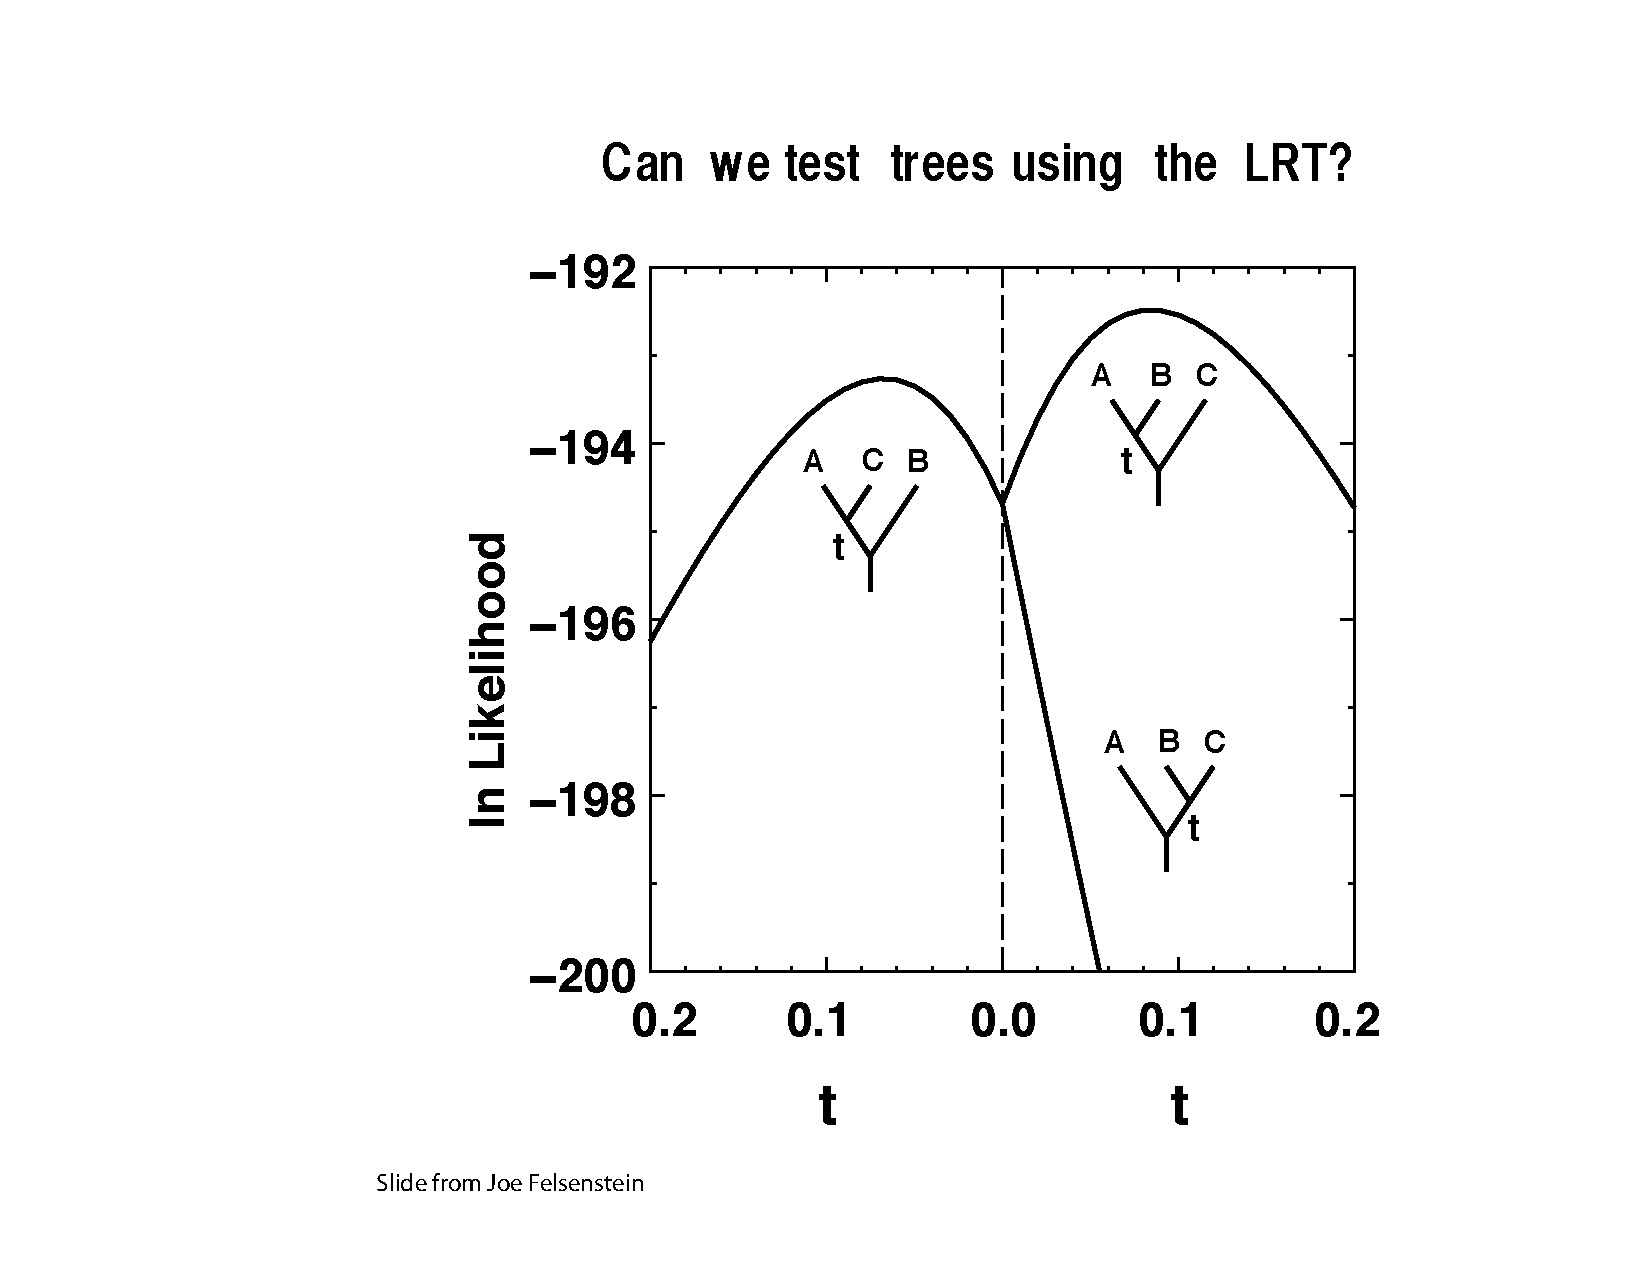
\includegraphics[scale=1.0]{../newimages/JoeFelsTreeLRT2.pdf}}}
\end{picture}

\myNewSlide
\section*{Parametric bootstrapping}
Generate the null distribution of $\delta_i$ by:
\begin{compactitem}
	\item finding the best tree and model pair that are consistent with the $H_0$,
	\item Simulating a large number $B$ of data sets, $X^{(1)}, X^{(2)},\ldots,X^{(B)}$ according to the parameters of that model,
	\item Calculating $\delta^{(j)} = 2\left[\ln L (\hat{T}| X^{(j)}) - \ln L (\hat{T}_{0}| X^{(j)})\right]$ where $\hat{T}_{0}$ is the tree estimated when you enforce a constraint such that all of the trees are compatible with the null.
\end{compactitem}

\myNewSlide
\section*{Parametric bootstrapping}
Intuitive and powerful, but not robust to model violation \citep{Buckley2002}.

In the SOWH test, the null tree is specified {\em a priori}.

\myNewSlide
\includepdf[pages={1}]{/Users/mholder/Documents/ku_teaching/BIOL-848-2010/images/gtr_i_g_sim_hist_data.pdf} 


\myNewSlide
\includepdf[pages={1}]{/Users/mholder/Documents/ku_teaching/BIOL-848-2010/images/jc_sim_hist_data.pdf} 

\myNewSlide
\section*{aLRT of \citet{AnisimovaG2006}}
\begin{compactitem}
	\item For a {\bf branch} $j$, calculate $\delta_{j}^{\dag}$ as twice the difference in $\ln L$ between the optimal tree (which has the branch) and the best NNI neighbor that lacks the branch.
	\item This is very fast, and can be done in PhyML.
	\item The argue that the null distribution for each LRT around the polytomy follows a $\frac{1}{2}\chi_0^2 + \frac{1}{2}\chi_1^2$ distribution
	\item The introduce Bonferroni-correction appropriate for correcting for the selection of the best of the three resolutions.
	\item They find aLRT to be accurate and powerful in simulations, but \citet{AnisimovaGDDG2011} report that it rejects too often and is sensitive to model violation.
\end{compactitem}

\myNewSlide
\begin{picture}(500,0)(0,0)
	  \put(-130,-450){\makebox(0,0)[l]{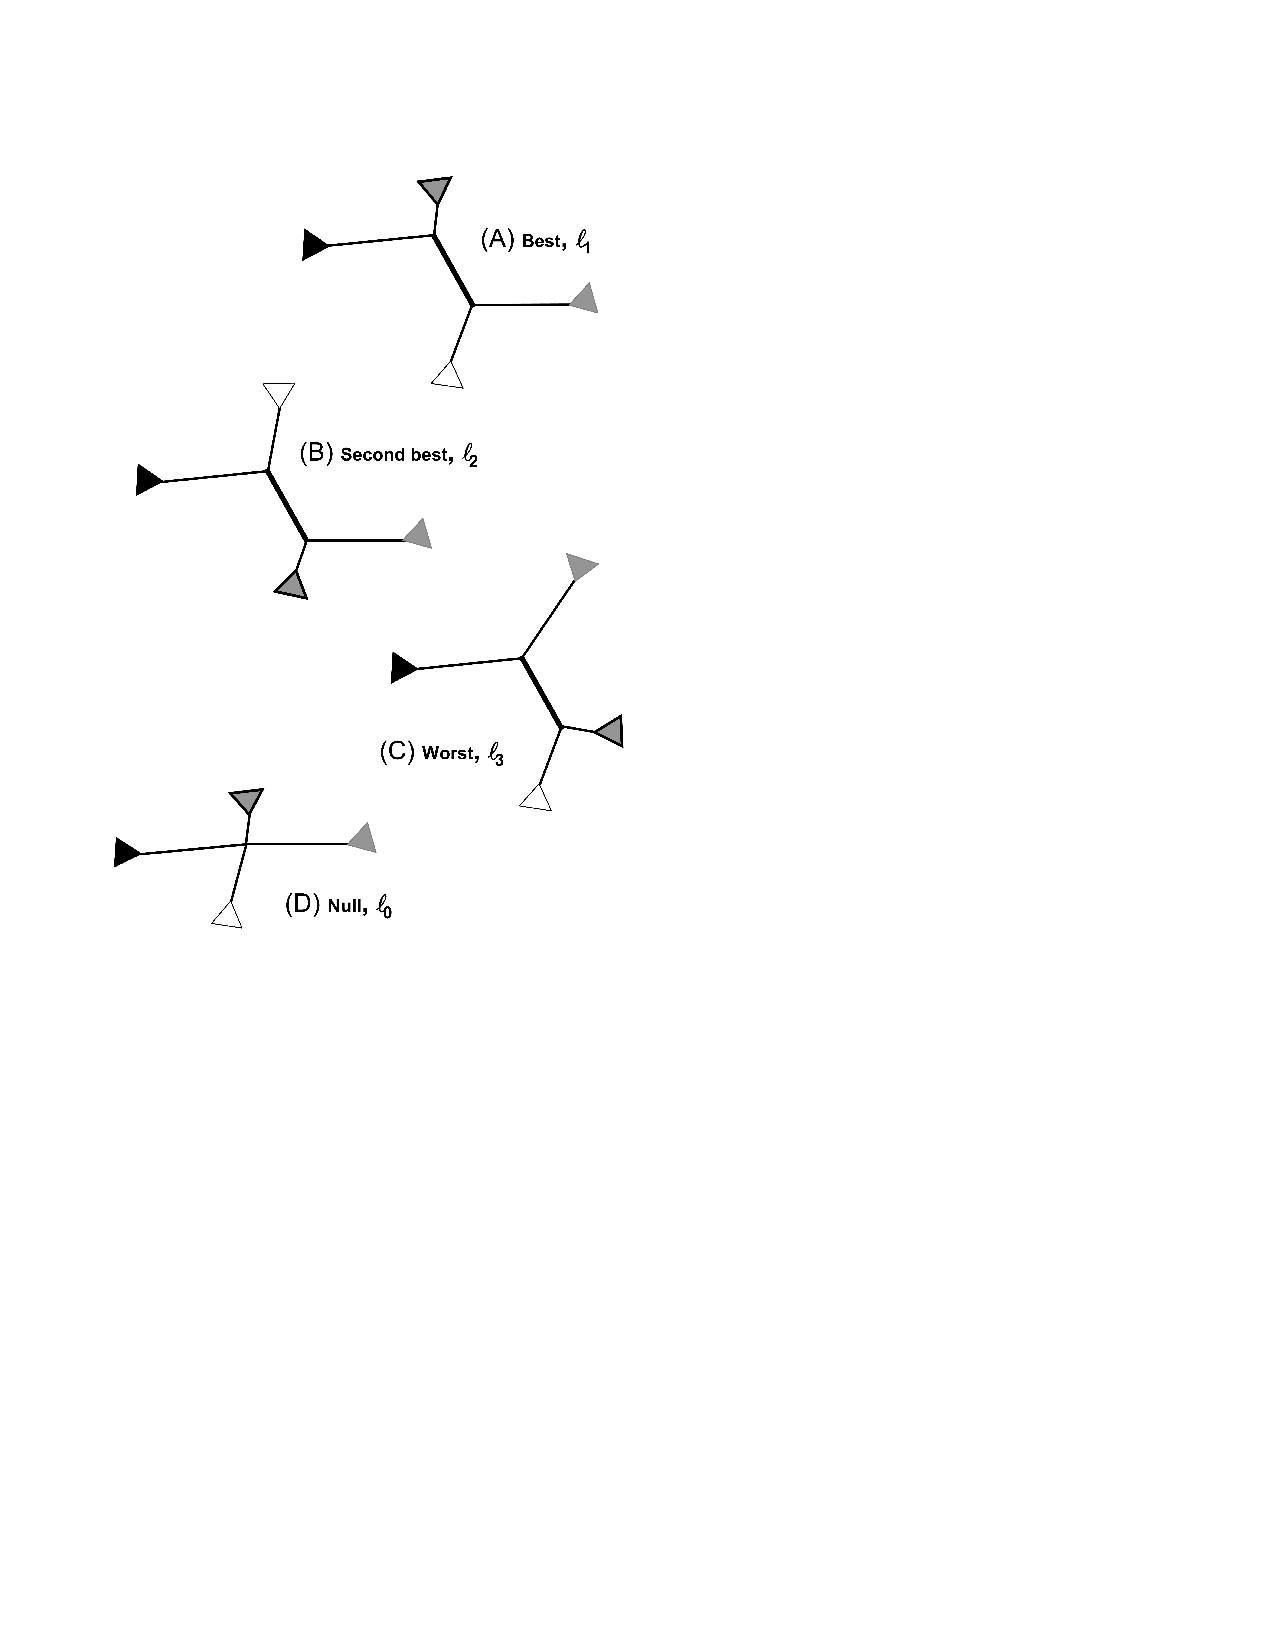
\includegraphics[scale=1.5]{../newimages/AnisimovaG2006Fig1.pdf}}}
	  \put(330,-200){aLRT = $2\left[\ln L(T_1|X) - \ln L(T_2|X)\right]$}
	  \put(400,-400){\small Image from \citet{AnisimovaG2006}}
\end{picture}

\myNewSlide
\section*{aBayes \citet{AnisimovaGDDG2011} }


$$\mbox{aBayes}(T_1|X) = \frac{\Pr(X|T_1}{\Pr(X|T_1) + \Pr(X|T_2) + \Pr(X|T_3)}$$

Simulation studies of \citet{AnisimovaGDDG2011} show it to have the best power of the methods that do not have inflated probability of falsely rejecting the null.

It is sensitive to model violation.

This is similar to ``likelihood-mapping'' of \citet{StrimmerVH1997}




\myNewSlide
\large
Bootstrap proportions have been characterized as providing:
\begin{compactitem}
	\item a measure of repeatability,
	\item an estimate of the probability that the tree is correct (and bootstrapping has been criticized as being too conservative in this context),
	\item the P-value for a tree or clade
\end{compactitem}





\myNewSlide
\section*{Bootstrap Proportion $\neq$ Posterior Probability}
Several studies have compared the non-parametric bootstrap proportion of clade from an ML analysis of a data set to the posterior probabilities when the same data is analyzed under the same model \citep{SuzukiGN2002,WilcoxZHH2002,AlfaroZL2003,CummingsHMRRW2003,DouadyDBDD2003}.\par

Note: {\em \bf Not} all of these have implied that the measures {\em\bf should} be the same, but some authors have, usually citing \citet{EfronHH1996}.

\myNewSlide
\section*{Bootstrap Proportion $\neq$ Posterior Probability in general}
\begin{picture}(-0,0)(-0,0)
	\put(40,-50){\makebox(30,-150)[l]{\includegraphics[scale=2]{/Users/mholder/Documents/ku_teaching/BIOL-848-2010/images/WilcoxZHH-figure.pdf}}}
	\put(40,-330){from \citet{WilcoxZHH2002}}
\end{picture}


\myNewSlide
\section*{\citet{Newton1996} showed that, when you look at the median, the BP may not be biased downward}
\begin{picture}(-0,0)(-0,0)
	\put(40,-50){\makebox(30,-150)[l]{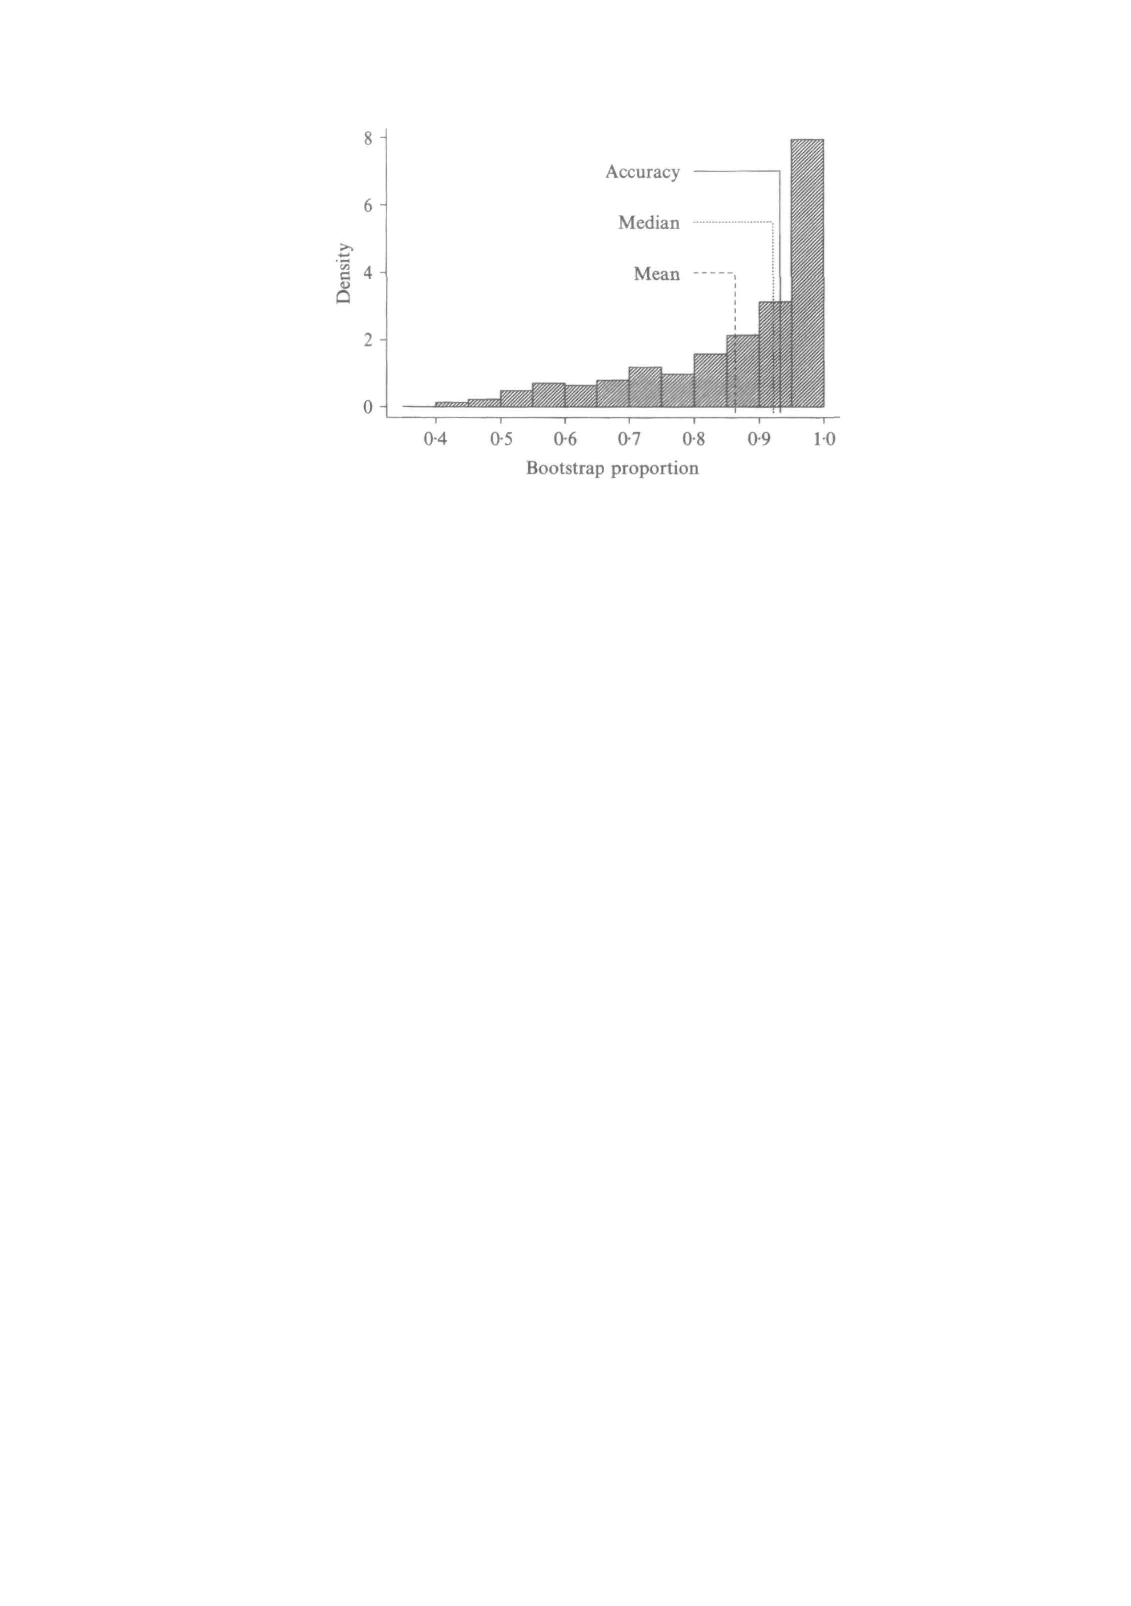
\includegraphics[scale=2]{../newimages/Newton1996Fig4.pdf}}}
	\put(40,-330){Figure 4 from \citet{Newton1996}}
\end{picture}

\myNewSlide
\section*{What did \citet{EfronHH1996} say?}
\normalsize
We can use a Bayesian model to show that $\tilde{\alpha}$ is a reasonable 
assessment of the probability that $\mathscr{R}_1$ contains $ \mu$.
Suppose we believe \textit{a priori} that $\mu$ could lie anywhere in the plane with 
equal probability. 
Then having observed $\hat{\mu}$, the \textit{a posteriori} 
distribution of  $\mu$ given  $\hat{\mu}$ is $N_2( \hat{\mu},I)$ exactly the same as the 
bootstrap distribution of $\hat{\mu}^{\ast}$. 
In other words, $\tilde{\alpha}$ is the  \textit{a posteriori}
probability of the event $\mu \in \mathscr{R}_1$, if we begin with an ``uninformative'' prior density for $\mu$.
\begin{picture}(-0,0)(-0,0)
	\put(0,-120){\makebox(30,-150)[l]{\includegraphics[scale=4]{/Users/mholder/Documents/ku_teaching/BIOL-848-2010/images/EfronHH-straight-fig.pdf}}}
\end{picture}

\myNewSlide
\section*{\citet{EfronHH1996} view of tree space}
\begin{picture}(-0,0)(-0,0)
	\put(-10,-90){\makebox(30,-150)[l]{\includegraphics[scale=3]{/Users/mholder/Documents/ku_teaching/BIOL-848-2010/images/EfronHH-treespace-fig.pdf}}}
\end{picture}

\myNewSlide
\section*{What did \citet{EfronHH1996} say (and mean)?}
\begin{itemize}
	\item the ``uninformative'' prior density is a uniform prior over all of pattern frequency space
	\item this is {\em not} equivalent to a prior that would be expected to yield a phylogeny (it is actually identical to the prior you would get if you assumed that all pairwise distances between taxa were $\infty$),
	\item  \citet{EfronHH1996}  were {\em not} predicting that the bootstrap proportions should be identical to those from a Bayesian phylogenetic analysis with real phylogenetic priors.
	\item  \cite{SvennbladEOB2006} have a nice paper on this subject.
\end{itemize}


\myNewSlide
\section*{\citet{Newton1996} provides an intuition for why the mean BP may be lower than repeatability}
\begin{picture}(-0,0)(-0,0)
	\put(40,-50){\makebox(30,-150)[l]{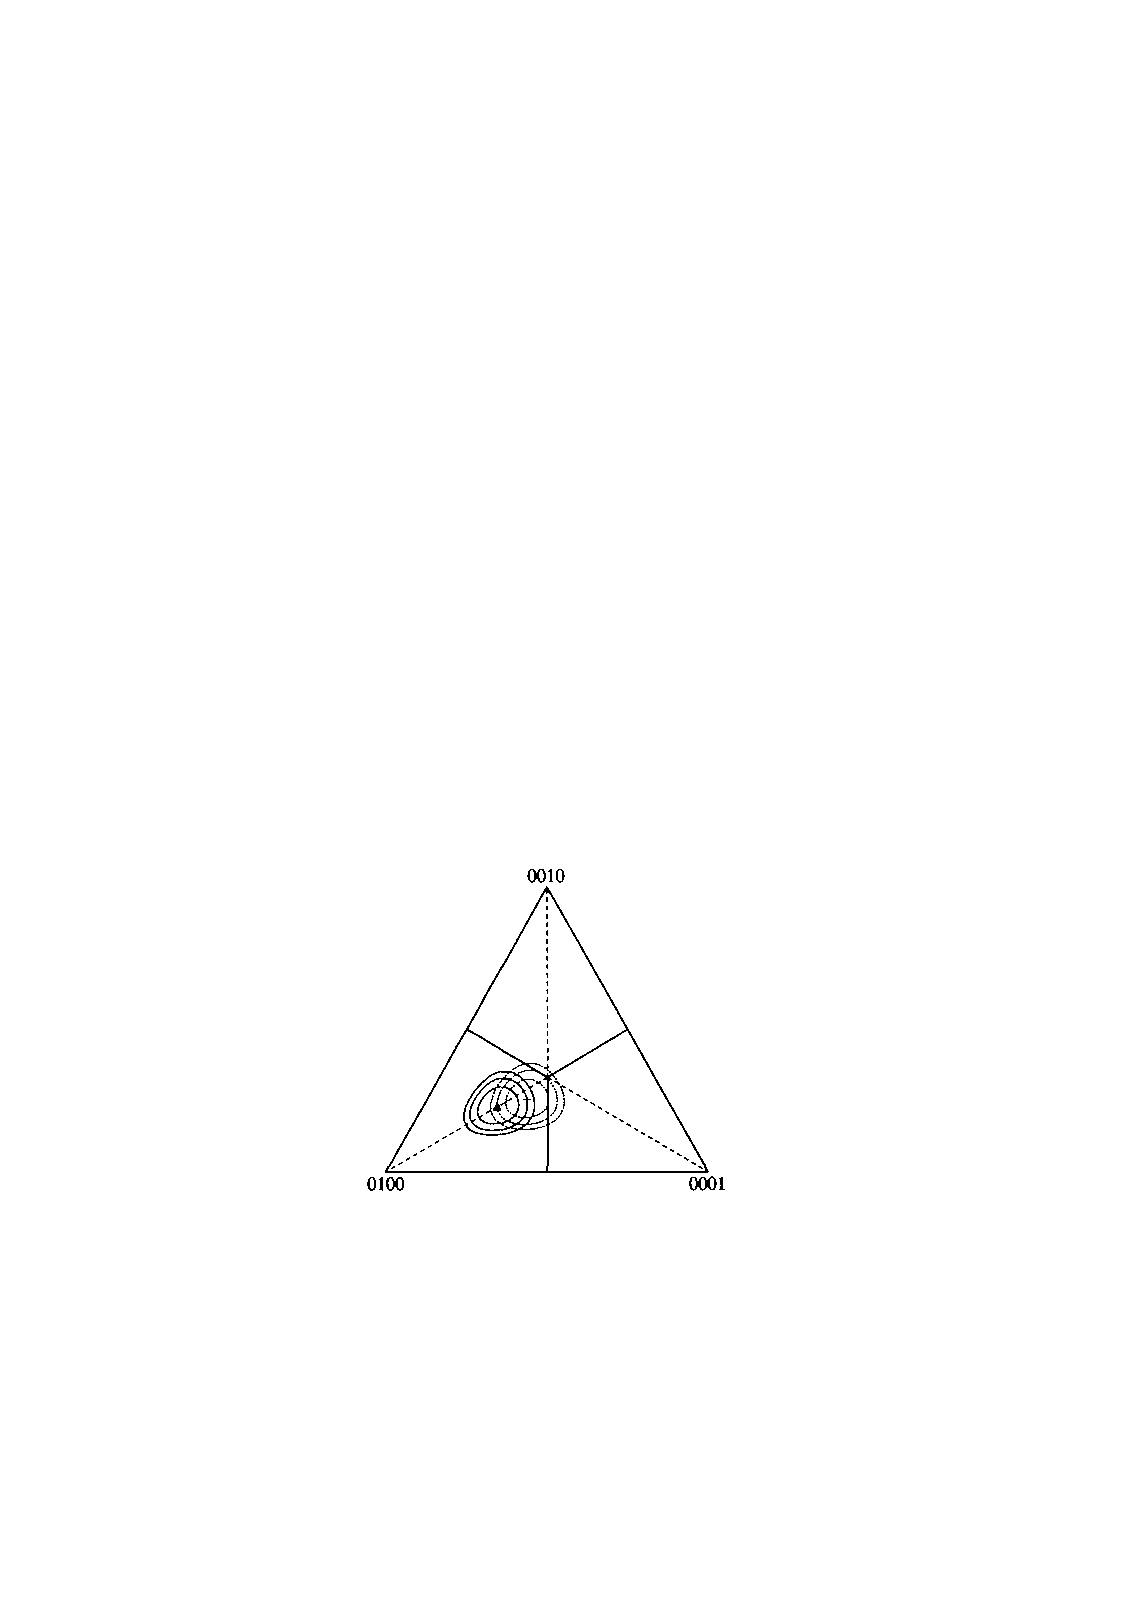
\includegraphics[scale=2]{../newimages/Newton1996Fig3.pdf}}}
	\put(40,-320){Darker ovals indicate probability contours for datasets given the truth}
	\put(60,-350){(note that repeatability $\approx$ 100\%)}
	\put(40,-380){Lighter ovals show probability contours for bootstrapping for one dataset.}
	\put(60,-410){Many real datasets will have BP much $<$ 100\%}
	\put(-40,-50){Figure 3 from \citet{Newton1996}}
\end{picture}



\myNewSlide
\large
Bootstrap proportions have been characterized as providing:
\begin{compactitem}
	\item {\color{grey} a measure of repeatability,}
	\item  {\color{grey} an estimate of the probability that the tree is correct (and criticized as being too conservative in this context),}
	\item the P-value for a tree or clade
\end{compactitem}




\myNewSlide
\section*{coin flipping (yet again)}
$N=100$ and $H=60$

Can we reject the hypothesis of a fair coin?

We can use simulation to generate the null distribution (we could actually use the binomial distribution to analytically solve this one)...

\myNewSlide

\begin{picture}(0,0)(0,0)
	\put(-10,-250){\makebox(0,0)[l]{\includegraphics[scale=1.0]{/Users/mholder/Documents/ku_teaching/BIOL-848-2010/images/nullhist.pdf}}}
	\put(180,-250){\color{red} P-value $\approx$ 0.029 }
\end{picture}

\myNewSlide
If we bootstrap we get a sense of the variability in our estimate, but we can also get a tail probability for $\Pr(p^{(boot)} \leq 0.5)$

\myNewSlide

\begin{picture}(0,0)(0,0)
	\put(-60,-250){\makebox(0,0)[l]{\includegraphics[scale=1.0]{/Users/mholder/Documents/ku_teaching/BIOL-848-2010/images/boothist.pdf}}}
	\put(60,-250){\color{red}$ \Pr(p^{(boot)} \leq 0.5)\approx$ 0.027 }
\end{picture}

\myNewSlide
\begin{picture}(-0,0)(-0,0)
	\put(60,00){\makebox(30,-150)[l]{\includegraphics[scale=0.5]{/Users/mholder/Documents/ku_teaching/BIOL-848-2010/images/nullhist.pdf}}}
	\put(60,-260){\makebox(30,-150)[l]{\includegraphics[scale=0.5]{/Users/mholder/Documents/ku_teaching/BIOL-848-2010/images/boothist.pdf}}}
\end{picture}



\includepdf[pages={28-45}]{/Users/mholder/Documents/ku_teaching/BIOL-848-2010/lec16-Bootstrapping/lec16Bootstrapping.pdf} 

\myNewSlide
\section*{\citet{EfronHH1996} view of tree space}
\begin{picture}(-0,0)(-0,0)
	\put(-10,-90){\makebox(30,-150)[l]{\includegraphics[scale=3]{/Users/mholder/Documents/ku_teaching/BIOL-848-2010/images/EfronHH-treespace-fig.pdf}}}
\end{picture}








\myNewSlide
\section*{\citet{Kim2000} view of tree space}
\begin{picture}(-0,0)(-0,0)
	\put(-10,-90){\makebox(30,-150)[l]{\includegraphics[scale=2.5]{/Users/mholder/Documents/ku_teaching/BIOL-848-2010/images/Kim-treespace.pdf}}}
\end{picture}

\myNewSlide
\section*{Parsimony-informative Pattern Frequency Space}
\begin{picture}(-0,0)(-0,0)
	\put(10,-140){\makebox(30,-150)[l]{\includegraphics[scale=1.]{/Users/mholder/Documents/ku_teaching/BIOL-848-2010/images/simple-treespace.pdf}}}
\end{picture}

\myNewSlide
\section*{Pattern Frequency Space With Observed Data}
\begin{picture}(-0,0)(-0,0)
	\put(10,-140){\makebox(30,-150)[l]{\includegraphics[scale=1.]{/Users/mholder/Documents/ku_teaching/BIOL-848-2010/images/simple-treespace-sample.pdf}}}
	\put(370,-183){$f_X$}
\end{picture}

\myNewSlide
\section*{Bootstrapping in Pattern Frequency Space}
\begin{picture}(-0,0)(-0,0)
	\put(10,-150){\makebox(30,-150)[l]{\includegraphics[scale=1.]{/Users/mholder/Documents/ku_teaching/BIOL-848-2010/images/simple-treespace-boot.pdf}}}
\end{picture}



\myNewSlide
\section*{\cite{Susko2010} adjusted BP -- aBP}
Susko reports that the curvature arguments of \citet{EfronHH1996} and \citet{Shimodaira2002}, while not incorrect, ignore the {\bf sharp point} in parameter space around the polytomy.

He uses the curvature of the likelihood function to correct bootstrap proportions so that $1-aBP$ accurately estimates the $P$-value.

You need to perform a different correction when you know the candidate tree {\em a priori} versus when you are putting BP on the ML tree.

BP may {\bf not} be conservative when you correct for selection bias.

\myNewSlide
\begin{picture}(-0,0)(-0,0)
	\put(-60,-150){\makebox(30,-150)[l]{\includegraphics[scale=0.75]{../scripts/Susko2010Table3aBP.pdf}}}
	\put(300,-150){\makebox(30,-150)[l]{\includegraphics[scale=0.75]{../scripts/Susko2010Table3aBPMLCorrection.pdf}}}
\end{picture}


\myNewSlide
\section*{aBP in Pattern Frequency Space}
\begin{picture}(-0,0)(-0,0)
	\put(-50,-0){Null distribution for BP}
	\put(-40,-30){is calculated using}
	\put(-40,-60){Normal approximations from}
	\put(-40,-90){polytomy}
	\put(10,-150){\makebox(30,-150)[l]{\includegraphics[scale=1.]{../newimages/simple-treespace-abp.pdf}}}
\end{picture}


\myNewSlide
\section*{ML scores in Pattern Frequency Space}
\begin{picture}(-0,0)(-0,0)
	\put(10,-120){\makebox(30,-190)[l]{\includegraphics[scale=1.]{../newimages/simple-treespace-pp1v2.pdf}}}
	\put(-30,-0){$\ln L(T_1|X) = -D_{KL}(f_X|f_{T_1})$}
\end{picture}

\myNewSlide
\section*{Bootstrapping in Pattern Frequency Space}
\begin{picture}(-0,0)(-0,0)
	\put(10,-150){\makebox(30,-150)[l]{\includegraphics[scale=1.]{/Users/mholder/Documents/ku_teaching/BIOL-848-2010/images/simple-treespace-boot.pdf}}}
\end{picture}

\myNewSlide
\section*{Bootstrapping in Pattern Frequency Space (if you had more data)}
\begin{picture}(-0,0)(-0,0)
	\put(-50,-0){AU Test uses multiple sequence}
	\put(-40,-30){lengths to correct BP for}
	\put(-40,-60){any curvature in the boundary }
	\put(-40,-90){between trees}
	\put(10,-150){\makebox(30,-150)[l]{\includegraphics[scale=1.]{../newimages/simple-treespace-boot-more.pdf}}}
\end{picture}

\myNewSlide
\section*{aLRT and aBayes in Pattern Frequency Space}
\begin{picture}(-0,0)(-0,0)
	\put(10,-120){\makebox(30,-190)[l]{\includegraphics[scale=1.]{../newimages/simple-treespace-ppv2.pdf}}}
	\put(-50,-0){In aLRT, we use mixtures of $\chi^2$}
	\put(-40,-30){and selection bias corrections}
	\put(-40,-60){to calculate the $P$-value.}
	\put(370,-0){In aBayes, we normalize}
	\put(380,-30){the ML scores to (0,1)}
\end{picture}

\myNewSlide
\section*{KH Test in Pattern Frequency Space}
\begin{picture}(-0,0)(-0,0)
	\put(10,-120){\makebox(30,-190)[l]{\includegraphics[scale=1.]{../newimages/simple-treespace-kh.pdf}}}
	\put(-50,-0){Uses the $\delta$ test statistic}
	\put(-40,-30){and a null distribution}
	\put(-40,-60){{\em centered} on the boundary}
\end{picture}

\myNewSlide
\section*{Parametric bootstrapping in Pattern Frequency Space}
\begin{picture}(-0,0)(-0,0)
	\put(10,-120){\makebox(30,-190)[l]{\includegraphics[scale=1.]{../newimages/simple-treespace-parametricBP.pdf}}}
	\put(-50,-0){Uses the $\delta$ test statistic}
	\put(-40,-30){and a null distribution}
	\put(-40,-60){{\em centered} on point that}
	\put(-40,-90){arises from the best}
	\put(-40,-120){tree in $H_0$}
\end{picture}


\myNewSlide
\section*{Summary - Part 1}

\begin{itemize}
	\item $\delta(T_1,T_2|X) = 2\left[\ln L(T_1|X) - \ln L(T_2|X)\right]$ is a powerful statistic for discrimination between trees.
	\item We can assess confidence by considering the variance in signal between different characters.
	\item Bootstrapping helps us assess the variance in $\ln L$ that we would expect to result from sampling error.
\end{itemize}

\myNewSlide
\section*{Summary - Part 2}
\normalsize
A (very) wide variety of tests differ by:
\begin{itemize}
	\item Null hypotheses:
	\begin{compactitem}
		\item Expected scores are the same $\rightarrow$ boundary tests. {\bf Non-parametric tests}
		\item A tree consistent with the null is correct $\rightarrow$ tests that use the full info of the model. {\bf Parametric tests}
	\end{compactitem}
	\item How to use variance information:
	\begin{compactitem}
		\item Rely on ``raw'' bootstrap variability,
		\item Invoke assumptions of normality of scores,
		\item Use $\chi^2$ variants.
	\end{compactitem}
	\item Whether or not the trees must be specified {\em a priori} -- KH Test requires the trees to be specified {\em a priori}.
\end{itemize}

\myNewSlide
\section*{Summary - Part 3}
\large
\begin{table}[htdp]
\begin{center}
\begin{tabular}{|c|p{7cm}|p{6cm}|}
\hline
& Parametric & Nonparametric \\
\hline
$P$-value from $\delta$  & aLRT, aBayes, parametric bootstrapping & KH, SH \\
\hline
$P$-value from BP $\delta$  &aBP(semi)  & BP, aBP(semi), AU, EHH\\
\hline
\end{tabular}
\end{center}
\label{default}
\end{table}%

When you use a parametric test, you will usually gain power. But non-parametric tests are more robust to model violation.



\myNewSlide
\normalsize
\bibliography{phylo}
\end{document}

